\documentclass[12pt]{article}
\usepackage[margin=1in]{geometry}
%\usepackage[margin=1.5in]{geometry}
\setlength{\parindent}{0em}
\setlength{\parskip}{0.5em}
\usepackage{setspace} % spacing between toc items
\usepackage{graphicx}
\usepackage{amsmath}
\usepackage{xcolor}
\definecolor{cadmiumgreen}{rgb}{0.0, 0.42, 0.24}
\definecolor{darkpowderblue}{rgb}{0.0, 0.2, 0.6}

%\usepackage[compact]{titlesec}
%   [<shape>]{<format>}{<label>}{<sep>}{<before-code>}[<after-code>]
\usepackage{titlesec}
\titleformat{\section}%
  %{\fontsize{16}{18}\selectfont\bfseries\color{myblue}}
  {\fontsize{16}{18}\selectfont\bfseries}
  {\arabic{section}\color{black}}
  {1em}{}
\titleformat{\paragraph}%
  {\bfseries}
  {Unit }
  {1em}{}
\titlespacing*{\section}{-0.75in}{0ex}{0ex}
\titlespacing*{\subsection}{-0.5in}{0ex}{0ex}
\titlespacing*{\paragraph}{0in}{0.5ex}{-1ex}

\usepackage{enumitem}
\setlist[itemize]{noitemsep}
\setlist[enumerate]{noitemsep}
\setlist[description]{%
    noitemsep,
    labelindent=1em,
    topsep=-1ex,
    font={\sffamily\bfseries\color{cadmiumgreen}}
}

\usepackage{hyperref}
\hypersetup{colorlinks=true,urlcolor=darkpowderblue, linkcolor=black}
\urlstyle{same}

\definecolor{myGreen}{rgb}{0.0,0.26,0.15}
\definecolor{om}{rgb}{0.4,0.19,0.28} % om - old mauve

\definecolor{myBlue}{rgb}{0.2,0.2,0.6}
\newcommand{\mynotes}[1]{\textcolor{myBlue}{#1}}

\definecolor{hl}{rgb}{0.61, 0.87, 1.0}
\newcommand{\test}[1]{%
    \begin{center}
        {\parbox{0.9\textwidth}{\textit{\small#1}}}
    \end{center}}

\definecolor{date}{HTML}{5F0087}
\newcommand{\mydate}[1]{
    \begin{flushright}
        \rule{\textwidth}{0.4pt} %{\vspace{-1ex}
        \small\hfill\textit{#1}
    \end{flushright}}


\title{\vspace{-0.75in}ASTR 535 Lecture Notes}
\author{Jon Holtzman}
\date{Spring 2016}

\begin{document}
\maketitle

course website: \url{http://astronomy.nmsu.edu/holtz/a535}

\renewcommand{\baselinestretch}{0.5}\normalsize
\tableofcontents
\renewcommand{\baselinestretch}{1.0}\normalsize

%\addtocontents{toc}{\protect\setstretch{0.1}}
%\tableofcontents

\newpage
\mydate{Friday, January 22}
\section{Properties of light, magnitudes, errors,\\
and error analysis}

\subsection{Light}
Wavelength regimes:
\begin{itemize}
    \item gamma rays
    \item x-rays
    \item ultraviolent (UV)
        \begin{itemize}
            \item near: 900--3500 \AA{}
            \item far: 100--900 \AA{}
        \end{itemize}
        The 900 \AA{} break is because of the Lyman limit at 912 \AA{}.
        This is where neutral hydrogen is ionized, so the universe is largely
        opaque to wavelengths shorter than this.
    \item visual (V): 4000--7000 \AA{}
    (note that `V' is different from `optical',
        which is slightly broader: 3500--10000 \AA{}. The 3500 \AA{} cutoff
        is due to the Earth's atmosphere being opaque to wavelengths shorter
        than this).
    \item IR
        \begin{itemize}
            \item near: 1--5 $\mu$ (1--10 $\mu$ in online notes)
            \item mid: (10--100 $\mu$)
            \item far: 5--100 $\mu$ (100--1000 $\mu$)
        \end{itemize}
    \item sub-mm 500--1000 $\mu$
    \item microwave
    \item radio
\end{itemize}
Quantities of light:
\begin{itemize}
    \item Intensity $I(\theta,\phi)$ [erg s$^{-1}\ \nu^{-1}\ \Omega^{-1}$]:
        Encapsulates $direction$ light is coming from.
        Also known as radiance.
    \item Surface Brightness (SB)
        [erg s$^{-1}$ cm$^{-2}$ $\nu^{-1}$ sterradian$^{-1}$]:
        amount of energy \emph{received} in a unit surface
        element per unit time per unit frequency (or wavelength)
        from a unit
        solid angle in the direction ($\theta,\phi$), where $\theta$
        is the angle
        away from the normal to the surface element, and $\phi$ is the
        azimuthal angle.
        To calculate SB, just divide the flux by the angle subtended
        by the object [rad$^{2}$]. At a larger distance, the flux will
        be smaller, but so will the angle subtended by the object, so
        SB is independent of distance unless considering cosmological
        scales, where the curvature of spacetime has an effect.
        \textcolor{red}{If SB is per unit \emph{area}, how is that
        independent of distance?}
    \item Flux (F) [erg s$^{-1}$ cm$^{-2}\ \nu^{-1}$]:
        amount of energy passing through a unit surface element
        in all directions, defined by
        \begin{equation}
            F_{\nu} = \int I_{\nu}\cos(\theta)\textrm{d}\Omega
        \end{equation}
        where d$\Omega$ is the solid angle element, and the integration is
        over the entire solid angle. Intensity is per solid angle. All
        the solid angles that make up a sphere add up (integrate) to
        get the total flux through that surface.
        The $\cos(\theta)$ factor is important
        for, e.g., ISM where light is coming from all directions, but for
        tiny objects, $\theta$ is negligibally small and can be dropped.
        Integrates over $all$ directions.
        Also known as irradiance. Can also be per $\lambda$, obviously.
    \item Luminosity (L) [erg s$^{-1}$]:
        $intrinsic$ energy emitted by the source per
        second ($\sim$ power). For an isotropically emitting source,
        \begin{equation}
            L = 4 \pi d^{2} F
        \end{equation}
        where $d$ = distance to source (so L can only be calculated if
        the distance is known). Also known as radiant flux.
\end{itemize}
What to measure for sources:
\begin{itemize}
    \item Resolved: directly measure surface brightness (intensity)
        distribution on the sky, usually over some bandpass or wavelength
        interval.
    \item Unresolved: measure the flux. Diffraction is the reason stellar
        surfaces cannot be resolved. Because of this, we cannot measure
        SB, so we measure flux, integrated over the entire object.
\end{itemize}

Questions:
\begin{itemize}
    \item What are the dimensions of the three quantities: luminosity,
        surface brightness (intensity), and flux?
    \item How do the three quantities depend on distance to the source?
    \item To what quantity is apparent magnitude of a star related?
    \item To what quantity is the absolute magnitude related?
\end{itemize}
\emph{specific} flux: per unit wavelength (or frequency).
Using $\lambda=\frac{c}{\nu} \rightarrow
\frac{\textrm{d}\lambda}{\textrm{d}\nu} = \frac{-c}{\nu^{2}}$
\begin{align*}
    \int F_{\nu} \textrm{d} \nu &= -\int F_{\lambda} \textrm{d} \lambda\\
    F_{\nu} \textrm{d} \nu &= -F_{\lambda} \textrm{d} \lambda\\
    F_{\nu} &= -F_{\lambda} \frac{\textrm{d} \lambda}{\textrm{d}\nu}\\
    &= F_{\lambda} \frac{c}{\nu^{2}}\\
    &= F_{\lambda} \frac{\lambda^{2}}{c}\\
\end{align*}
The negative comes from frequency and wavelength increasing in
opposite directions.
Note that a constant $F_{\lambda}$ implies a \emph{non}-constant $F_{\nu}$
and vice versa. For example, a wavelength difference of 100 \AA{}
around 1215 \AA{} and 6563 \AA{} corresponds to a frequency difference
of 2200 GHz and 71 GHz, respectively.

Units: cgs, magnitudes, Jansky (a flux density unit:
1 Jy = $10^{-26}$ W m$^{-2}$ Hz$^{-1}$)

Terminology of measurements:
\begin{itemize}
    \item photometry (broad-band flux measurement): SB or flux, integrated
        over some wavelength range.
    \item spectroscopy (\emph{relative} measurement of fluxes at
        different wavelengths):
        $f(\lambda)$
    \item spectrophotometry (\emph{absolute} measurement of fluxes at
        different wavelengths):
        $f(\lambda)$
    \item astrometry: concerned with positions of observed flux, not brightness,
        but direction.
    \item morphology: intensity as a function of position;
        often, absolute measurements are unimportant. Deals with $resolved$
        objects, intensity as function of position.
\end{itemize}
In general:
\begin{itemize}
    \item photometry: measure \emph{flux}
    \item spectroscopy: flux \emph{density} (per unit wavelength,
        down to the resolution of the spectrograph)
\end{itemize}

In practice, measure \emph{photon} flux [photons cm$^{-2}$ s$^{-1}$]
with a ``photon counting device'',
(rather than energy flux, which is done with bolometers).
The monochromatic photon flux is given by the
energy flux ($F_{\lambda}$) divided by the
energy per photon ($E_{photon} = \frac{hc}{\lambda}$), or
$$ \textrm{photon\ flux} = \int F_{\lambda}
    \frac{\lambda}{hc} \textrm{d} \lambda $$

\textcolor{om}{\emph{Have a complete understanding of the difference between
intensity, flux, and luminosity and their units. Recognize and
understand that these can be specified per unit wavelength or per unit
frequency and how to convert between the two.}}

%-----------------------------------------------------------------------%

\subsection{Magnitudes and photometric systems}
Magnitudes are related to flux (or SB or L) by:
    $$  m_1 - m_2 = -2.5 \log \frac{b_1}{b_2} $$
or for a single object:
\begin{align*}
    m &= -2.5 \log \frac{F}{F_0}\\
      &= -2.5 \log F + 2.5 \log F_0
\end{align*}
where the coefficient of proportionality, $F_0$, depends on the definition
of the photometric system, and the quantity $2.5\log{F_0}$ may be referred to as
the photometric system \emph{zeropoint}.
(Note that this relationship holds
\emph{regardless of what photometric system you are using}.
Inverting, we get:
    $$ F = F_{0} \times 10^{-0.4\textrm{m}} $$

Flux \emph{density}: flux per unit wavelength/frequency
(aka \emph{monochromatic} flux as opposed to integrated flux).
This can be specified by monochromatic magnitudes:
\begin{equation*}
    F_{\lambda} = F_0 (\lambda) \times 10^{-0.4 \textrm{m}(\lambda)}
\end{equation*}
although spectra are more often given in flux units than in magnitude units.
Note that it is possible that $F_0$ is a function of wavelength.

Since magnitudes are logarithmic, the \emph{difference} between
magnitudes corresponds to a \emph{ratio} of fluxes; ratios of magnitudes are
generally unphysical. If one is just doing relative measurements of
brightness between objects,
\textcolor{red}{this can be done without knowledge of $F_0$
(or, equivalently, the system zeropoint); objects that differ in brightness
by $\Delta$M have the same ratio of brightness (10$^{-0.4 \Delta M}$)
regardless of what photometric system they are in.
The photometric system definitions and zeropoints are only needed when
converting between calibrated magnitudes and fluxes.}
In other words, if you reference the
brightness of A relative to the brightness of B, a magnitude system
can be set up with B as the reference source.
However, the utility of a system when doing astrophysics generally
requires an understanding of the actual fluxes.

\textcolor{om}{\emph{Know how magnitudes are defined, and that
\underline{relative} fluxes can be represented as magnitudes independent of the
magnitude system.}}

\textcolor{date}{Monday, January 25}

Three main types of magnitude systems in use in astronomy:
\begin{enumerate}
    \item STMAG
    \item ABNU
    \item UBVRI
\end{enumerate}
The STMAG and ABNU magnitude systems are the simplest.
In these systems, the reference flux is just some \emph{constant} value in
$F_{\lambda}$ or $F_{\nu}$. However, these are not always the most widely used
systems in astronomy, because
\textcolor{red}{no natural source exists with a flat spectrum}.

\textbf{STMAG (Space Telescope MAGnitude) system:}
defined relative to $F_{\lambda}$. The reference flux is given by
$$    F_{0,\lambda} = 3.60 \times 10^{-9}\ \textrm{erg\ s}^{-1}\
    \textrm{cm}^{-2}\ \textrm{\AA{}}^{-1} $$
which is equal to the flux of Vega at $\lambda = 5500$ \AA{};
hence a star of Vega's brightness at 5500 \AA{} is defined to have m=0
(i.e., if $F = F_{0}$, then $m=\log(F/F_{0}) = \log(1) = 0$).
Alternatively (using $m = -2.5\log \frac{F}{F_0}$):
$$    m_{\textrm{STMAG}} = -2.5 \log F_{\lambda} - 21.1 $$
for $F_{\lambda}$ in \textcolor{red}{cgs units} (using cm$^{-2}$ \AA{}$^{-1}$
distinguishes between the collecting area and the wavelength, since both are
units of distance. Be careful with units when doing these conversions; as
long as the proper flux units come out at the end, the answer should be
correct).

\textbf{ABNU system:}
defined relative to $F_{\nu}$. The reference flux is given by
$$ F_{0,\nu} = 3.63 \times 10^{-20}\ \textrm{erg\ s}^{-1}\
    \textrm{cm}^{-2}\ \textrm{Hz}^{-1} = F_{\nu,Vega} $$
or
$$     m_{\textrm{ABNU}} = -2.5 \log F_{\nu} - 48.6 $$
for $F_{\nu}$ in \textcolor{red}{cgs units}.

Magnitudes usually refer to the \emph{integrated} flux (over a
spectral bandpass, not just a single wavelength).
The STMAG and ABNU integrated systems are defined relative to sources
of \emph{constant} $F_{\lambda}$ and $F_{\nu}$, respectively
\begin{align*}
    m_{\textrm{STMAG}} &= -2.5 \log \frac{\int F_{\lambda} \lambda
    \textrm{d}\lambda}{\int3.6\times10^{-9}\lambda\textrm{d}\lambda}\\
    m_{\textrm{ABNU}} &= -2.5 \log \frac{\int F_{\nu}\nu^{-1}
\textrm{d}\nu}{\int 3.6 \times 10^{-20}\nu^{-1}\textrm{d}\nu}
\end{align*}
These are defined to be the same at 5500 \AA{}.
The factors of $\lambda$ and $\nu$ come from the conversion factor
$hc/\lambda$ for photon-counting detectors, where $h$ and $c$ cancel
in each flux ratio.

Note that these systems differ by more than a constant,
because one is defined by units of $F_{\lambda}$ and the other by $F_{\nu}$,
so the difference betwen the systems is a function of wavelength.
(Question: what's the relations between $m_{STMAG}$ and $m_{ABNU}$?)

Note also that, using magnitudes,
\textcolor{red}{the measured magnitude is
nearly independent of bandpass width}, so a broader bandpass does not
imply a brighter (smaller) magnitude, which is not the case for
fluxes. The reference is being integrated as well, so they cancel.

The standard UBVRI broadband photometric system, as well as
several other magnitude systems, however, are not defined for a
constant (flat) $F_{\lambda}$ or $F_{\nu}$ spectrum; rather, they are defined
relative to the spectrum of an A0V star. Most systems are defined (or
at least were originally) to have the magnitude of Vega be zero in all
bandpasses (VEGAMAGS); if you ever get into this in detail, note that
this is not exactly true for the UBVRI system.

For the broadband UBVRI system, we have
$$    m_{\textrm{UBVRI}} \approx -2.5 \log
    \frac{\int_{UBVRI}F_{\lambda}(object)\lambda\textrm{d}\lambda}
    {\int_{UBVRI}F_{\lambda}(Vega)\lambda\textrm{d}\lambda} $$
(as above, the factor of $\lambda$ comes in for photon counting
detectors). This gives the magnitude in U, B, V, R, \emph{or} I,
by integrating over that same bandpass.
The UBVRI filter set had overlapping bandpasses, so
there was a switch to interference filter: the ugriz system used
by SDSS\@.

Here is a
\href{http://astronomy.nmsu.edu/holtz/a535/html/diagrams/a535/mag.htm}
{\textcolor{blue}{plot}}
to demonstrate the difference between the different systems.

While it seems that STMAG and ABNU systems are more
straightforward, in practice it is difficult to measure absolute
fluxes, and much easier to measure relative fluxes between objects.
Historically, observations were tied to observations of Vega (or
to stars which themselves were tied to Vega), so VEGAMAGs made sense,
and the issue of determining physical fluxes boiled down to measuring
the physical flux of Vega. Today, in some cases, it may be more
accurate to measure the absolute throughput of an instrumental system,
and use STMAG or ABNU.

\textcolor{om}{\emph{Know that there are several different magnitude
systems in use, and understand how they differ. Know when it is
important to know what the magitude system is, and when it isn't.}}

%-----------------------------------------------------------------%
\subsubsection{Colors}
In the UBVRI system, the \emph{difference} between magnitudes
(e.g.\ B-V) gives the ratio of the fluxes in different bandpasses
($F_{B}/F_{V}$)
\emph{relative to the ratio of the fluxes of
an A0V star in the same two bandpasses} (for VEGAMAG).
Note the typical colors of astronomical objects,
which are different for the different photometric systems.
Type `A' stars have color =  0, and have the same SED as Vega.
Type `O' stars have color $<$ 0,
while cooler stars have color $>$ 0.

Sloan system: ugriz (g-r=0 indicates constant $F_{\nu}$).
$$    m = -2.5\log\frac{\int_B F_{\lambda}\textrm{d}\lambda}
    {\int_V F_{\lambda}\textrm{d}\lambda} $$
if B-V=0, then (B/V)$_{object}$ is the same as (B/V)$_{Vega}$,
or $\left(\frac{\int F_{\nu}}{\int F_{\lambda}}\right)_{obj} =
    \left(\frac{\int F_{\nu}}{\int F_{\lambda}}\right)_{Vega} $.
An object with B-V=0 has the same spectral \emph{shape} as Vega.
Not necessarily the same flux value at each bandpass
Keep in mind that the UBVRI system is defined relative to spectrum of
an A0V star (not simply a flat spectrum, like the STMAG and ABNU
systems).

To know how much observing time is needed, you need to know the flux
for object with some magnitude, x.
E.g., convert the spectrum of an elliptical galaxy to color;
if you know $F$ in one filter, you can get $F$ in another filter.

Questions:
\begin{itemize}
    \item Which is closer to the UBVRI system, STMAG or ABNU?
    \item What would typical colors be in a STMAG or ABNU system?
\end{itemize}

\textcolor{om}{\emph{Understand how colors are represented by a difference in
magnitude, and recognize how colors expressed in magnitude are related
to the shape of the underlying spectrum, with differences for
different magnitude systems.}}

%-----------------------------------------------------------------%
\subsubsection{UBVRI magnitudes-flux conversion}
\textcolor{date}{Wednesday, January 27}

To \textcolor{red}{convert Vega-based magnitudes to fluxes},
just look up the flux of Vega at the center of the passband.
However, if the spectrum of the object
differs from that of Vega, this won't be perfectly accurate.
Given UBVRI magnitudes of an object in the desired band, filter profiles
(e.g. Bessell 1990, PASP 102,1181), and absolute spectrophotometry of
Vega (e.g., \href{http://adsabs.harvard.edu/abs/2004AJ....127.3508B}),
{\textcolor{blue}{Bohlin \& Gilliland 2004, AJ 127, 3508}},
one can determine the flux.

To estimate the flux of some object in
an arbitrary bandpass given just the V magnitude of an object (a common
situation used when trying to predict exposures times, see below),
estimate the spectral energy distribution (SED).
The integral of the SED can be computed over the V bandpass if the
filter profiles are known.
The scaling is determined by comparing this integral with that of
the spectrum of Vega over the same bandpass.
The normalized SED is then used to compute the flux in any
desired bandpass.

(Some possibly useful references for SEDs are:
Bruzual, Persson, Gunn, \& Stryker; Hunter, Christian, \& Jacoby;
Kurucz). Things are certainly simpler in the ABNU or STMAG system, and
there has been some movement in this direction: the STScI gives STMAG
calibrations for HST instruments, and the SDSS photometric system is
close to an ABNU system.
However, even when the systems are conceptually
well defined, determining the absolute calibration of any photometric
system is very difficult in reality, and determining absolute fluxes
to the 1\% level is very challenging.

As a separate note on magnitudes themselves, note that some
people, in particular, the SDSS, have adopted a modified type of
magnitudes, called \emph{asinh} magnitudes, which behave like normal (also
known as Pogson) magnitudes for brighter objects, but have different
behavior for very faint objects (near the detection threshold). See
\href{http://adsabs.harvard.edu/abs/1999AJ....118.1406L}
{\textcolor{blue}{Lupton, Gunn, \& Szalay 1999 AJ 118, 1406}}
for details.

%---------------------------------------------------------------%
\subsection{Observed fluxes and the count equation}
If you are measuring flux with an actual instrument,
the \emph{intrinsic} photon flux from the source is not
trivial to determine from the number of photons that you count.
To get the number of photons that you count in an observation,
you need to take into account
\begin{itemize}
    \item The area of your photon collector (telescope)
    \item Photon losses and gains from the Earth's atmosphere
    (which change with conditions)
    \item The efficiency of your collection/detection
    apparatus (which can change with time).
\end{itemize}
Generally, the astronomical signal (which might be a flux or a
surface brightness, depending on whether the object is resolved)
can be written in the form of the \emph{\textbf{count equation:}}
    $$ S = Tt \int \frac{F_{\lambda}}
    {\left(\frac{hc}{\lambda}\right)}q_{\lambda}
    a_{\lambda}\textrm{d}\lambda \equiv TtS' $$
    \begin{itemize}
        \item $S$: total number of photons observed (the ``signal'')
        \item $S'$: observed flux rate [photons s$^{-1}$ cm$^{-2}$],
            with all of the real details of the observing system included.
        \item $a_{\lambda}$: atmospheric transmission
            (or \emph{throughput}), the fraction of photons that
            make it to the detector.
            A typical value is about 0.9, or $\sim$90\% of the photons.
            Variable in both space and time.
        \item $q_{\lambda}$: system efficiency
            (telescope, instrument, filters, and detector). Can be
            time-variable.
        \item $T$: telescope collecting area
        \item $t$: integration time
            (total amount of time spent collecting photons).
        \item $\frac{F_{\lambda}}{\left(hc/\lambda\right)}$:
            flux divided by the energy per photon;
            gives the number of photons per second per square cm.
    \end{itemize}
$T$ and $t$ are the \emph{only} terms that do not depend on
the wavelength (or frequency).

Most of this information isn't needed to go
backward from $S$ to $F_{\lambda}$, since
the terms can be very difficult to measure precisely.
Instead, most observations are performed differentially to a
set of other stars of well-known brightness. If the stars of known
brightness are observed in the same observation, then the atmospheric
term is (approximately) the same for all stars.
This is known as
\emph{differential photometry}.
From the photon flux of the object with known brightness,
an ``exposure efficiency'' or an ``effective area'' for this
exposure can be determined.
Equivalently, and more commonly, an
\emph{instrumental magnitude} can be calculated:
    $$  m = -2.5 \log \frac{S}{t} $$
Normalize by the exposure time, $t$, to get counts s$^{-1}$,
(although this is not strictly necessary).
Then determine the \emph{zeropoint}, $z$ (which describes the
throughput of the system).
Adding $z$ to the instrumental magnitude gives the
\emph{calibrated} magnitude, $M$
(which is still an \emph{apparent} magnitude).
    $$ M = m + z $$
Note that in the real world, one has to also consider possible
differences between a given experimental setup and the setup used to
measure the reference brightnesses, so this is only a first
approximation (i.e., the zeropoint may be different for different
stars with different spectral properties). If using instrumental mags
including exposure time normalization, the zeropoint gives the
magnitude of a star that will give 1 count s$^{-1}$.
    $$ M = -2.5\log\frac{S}{t}+z $$

Example: to go from observed to emitted $\rightarrow$,
take an additional observation of an object with known brightness
(SDSS has list of these).
A star that is 10 times fainter than one with g=18 has g=20.5.
    $$ m = -2.5 \log(qF)$$
    $$ m = -2.5 \log F - 2.5\log q $$
the quantity `$-2.5\log q$' is the zeropoint.

If there is no nearby star, $q$ is still the same, but changes in $a$,
effects of the atmosphere, need to be calibrated.
This is known as \emph{all-sky}, or absolute, photometry.
This requires that the sky is ``well-behaved'',
i.e., the atmospheric throughput as a function of position can be
accurately predicted, which requires \emph{photometric} weather
(no clouds).
Differential photometry can be done in non-photometric weather,
hence it is much simpler. It is always possible to obtain
differential photometry, then later obtain absolute
photometry of the reference stars.

To figure out what the fluxes of the calibrating stars actually are
requires understanding all of the terms in the count equation.
This is challenging, and often absolute calibration of a system is
uncertain to a couple of percent.

It is common to stop with differential photometry when studying
variable objects, where only the \emph{change} in brightness is
important. In this case, the brightness of the target needs to be
referenced relative to another object (or ensemble of objects)
in the field that are \emph{non}-variable.

While the count equation isn't usually used for calibration,
it is very commonly used for computing the approximate number of
photons you will receive from a given source in a given amount of time
for a given observational setup. This number is critical to know in
order to estimate your expected errors and exposure times in observing
proposals, observing runs, etc. Understanding errors in absolutely
critical in all sciences, and maybe even more so in astronomy, where
objects are faint, photons are scarce, and errors are not at all
insignificant. The count equation provides the basis for
\textbf\emph{exposure time calculator} (ETC) programs,
because it gives $N_{\textrm{photons}}(t)$.
As we will see shortly, this provides the information we need to
calculate the \emph{uncertainty} in the measurement
as a function of exposure time.

Random note: The field of view (FOV) is usually in arcminute scales.

\textcolor{om}{\emph{Understand the count equation and the terms in
it. Understand the distinction between estimating count rates from an
understanding of all the terms in the count equation vs.\ measuring the
overall throughput (zeropoint) by observing stars of known brightness.
Know instrumental magnitudes and zeropoints are.}}
%-----------------------------------------------------------------------%
\subsection{Uncertainties in photon rates}
Useful reference:
\href{http://users.wfu.edu/ecarlson/skeptic/statistics.pdf}
{\textcolor{blue}{Statistics}}

For a given rate of \emph{emitted} photons, there's a probability function
which gives the rate of \emph{detected} photons.
Even assuming 100\% detection efficiency, there are still
\emph{statistical} uncertainties, and possibly \emph{instrumental}
uncertainties.

\textbf{\emph{General probability distributions and their
characteristics}}

$p(x)dx \equiv$ probability of event occuring in $x + \textrm{d}x$:
        $$ \int p(x)\textrm{d}x = 1 $$
Some definitions relating to values that characterize a distribution:
$$    \textrm{mean} \equiv \mu = \int xp(x)\textrm{d}x $$
$$    \textrm{variance} \equiv \sigma^{2} = \int (x-\mu)^{2} p(x)\textrm{d}x $$
$$    \textrm{standard\ deviation} \equiv \sigma =
        \sqrt{\textrm{variance}} $$
$$    \frac{ \int_{-\infty}^{x_{median}} p(x)\textrm{d}x }
      { \int_{-\infty}^{\infty} p(x)\textrm{d}x }
      = \frac{1}{2} $$
mode: most probable value (peak in plot).

\textcolor{date}{Monday, February 1}

Note that the geometric interpretation of the above (well-defined)
quantities depends on the nature of the distribution.
There is a difference between the \emph{sample} quantities
and the \emph{population} quantities. The latter apply
to the true distribution, while the former are \emph{estimates} of the latter
from some finite sample ($N$ measurements) of the population.
The sample values approach the true ones as $N$
approaches infinity, but for small samples, they may differ.

The sample quantities are derived from:
$$\textrm{sample\ mean:\ } \bar{x} \equiv \frac{\sum x_i}{N}$$
$$\textrm{sample\ variance:\ } \equiv
  \frac{\sum (x_i-\bar{x})^{2}}{N-1} =
  \frac{\sum x_i^{2}-(\sum x_i)^{2}/N}{N-1}$$

\textbf{\emph{the binomial distribution}}

For astronomical observations, the photon distribution can be derived from the
\emph{binomial} distribution:
   $$ P(x,n,p) = \frac{n!p^x(1-p)^{n-x}}{x!(n-x)!}  $$
where
\begin{itemize}
    \item $x$: number of photons in a single event
    \item $n$: total number of events
    \item $p$: probability of observing $x$
\end{itemize}
under the assumption that all events are independent of each other
(e.g., when rolling dice, the result of the second roll is independent
of the result of the first). For the binomial distribution:
   $$ \textrm{mean} \equiv \mu \equiv \int xp(x)\textrm{d}x = np $$
   $$ \textrm{variance} \equiv \sigma^{2} \equiv
      \int (x-\mu)^{2}p(x)\textrm{d}x = np(1-p) $$

\textcolor{om}{\emph{Understand the concept of probability
distribution functions and basic quantities used to describe them:
mean, variance, standard deviation, median, and mode. Understand the
difference between population quantities and sample quantities.}}

\textbf{\emph{The Poisson distribution}}

Unlike a gaussian, a poisson distribution is not
symmetric about the mean (you can't detect a negative number of
photons); it cuts off at zero.

For photon detection, $n$ is the total number of
photons emitted, and $p$ is the probability of detecting a
single photon out of the total emitted during the observation.
We don't know either of these numbers, but we do know that
\textcolor{red}{p$<<$1} and we can estimate the mean number detected:
  $$  \mu = np $$
In this limit, the binomial distribution asymtotically approaches the
\emph{Poisson} distribution:
   $$  P(x,\mu) = \frac{\mu^x e^{-\mu}}{x!} $$
From the expressions for the binomial distribution in this limit, the
mean of the distribution is $\mu$, and the variance is given by:
  $$  \sigma^{2} = \sum_x [(x-\mu)^{2}p(x,\mu)] $$
  $$  \sigma^{2} = np = \mu  $$

In other words, the standard deviation, $\sigma$, is the square root
of the mean.
\textcolor{red}{\textbf{This is an \emph{important result}}}.

Note that the Poisson distribution is generally the
appropriate distribution for \emph{any} sort of counting experiment
where a series of events occurs with a known average rate,
and are independent of time since the last event.

\href{http://astronomy.nmsu.edu/holtz/a535/html/diagrams/a535/poisson.htm}
{\textcolor{blue}{Plots}} of what the Poisson distribution looks like
for $\mu$ = 2, $\mu$ = 10, $\mu$ = 10000.

\textcolor{om}{\emph{Understand the Poisson distribution and when it
applies. Know how the variance/standard deviation of the Poisson
distribution is related to the mean of the distribution.}}

\textbf{\emph{The normal, or Gaussian, distribution}}

For large $\mu$, the Poisson distribution is
well-approximated around the peak by a Gaussian distribution:
    $$ P(x,\mu,\sigma) = \frac{1}{\sigma\sqrt{2\pi}}
        e^{ -\frac{1}{2} (\frac{x-\mu}{\sigma})^{2} }  $$
This allows us to use ``simple'' least squares
techniques to fit observational data, which is normally distributed.
However, in the \emph{tails of the distribution},
and at \emph{low mean rates}, the Poisson can
differ significantly from a Gaussian. In these cases,
least-squares may not be appropriate to model observational data,
maximum likelihood techniques need to be considered.

\emph{central limit theorem}: if a quantity
depends on a number of independent random variables with ANY
distribution, the quantity itself will be distributed normally (see
statistics texts). In observations, we encounter the normal
distribution because \emph{readout} noise is distributed normally.
Normal distributions occur often in nature.

\textcolor{om}{\emph{Know what a Gaussian is, including the full
functional form. Understand under what circumstances the Poisson
distribution is similar to a normal distribution.}}

\textbf{\emph{Importance of error distribution analysis}}

The expected uncertainties in observations need to be understood in
order to:
\begin{itemize}
    \item predict the amount of observing time needed to get
        uncertainties as small as they need to be.
    \item Figure out if the scatter in the observed data is consistent
        with expected uncertainties. If not, then
        you've either learned some astrophysics or you don't understand
        something about your observations. This is especially important in
        astronomy where objects are faint and many projects are pushing
        down into the noise as far as possible. This can usually only
        be answered probabilistically. Generally, tests compute the
        probability that the observations are consistent with an expected
        distribution (the null hypothesis). If it is low, the null
        hypothesis can be rejected.
    \item interpret your results in the context of a scientific prediction
\end{itemize}

\textbf{\emph{Confidence levels}}

For example, say we want to know whether some single point
is consistent with expectations, e.g., we see a bright point in
multiple measurements of a star, and want to know whether the star
flared. Say we have a time sequence with known mean and variance, and
we obtain a new point, and want to know whether it is consistent with
known distribution?

If the form of the probability distribution is known, then
you can calculate the probability of getting a measurement more than
some observed distance from the mean. In the case where the observed
distribution is Gaussian (or approximately so), this is done using the
\emph{error function} (sometimes called $erf(x)$), which is the integral of a
gaussian from some starting value.

Some simple guidelines to keep in mind follow (the actual
situation often requires more sophisticated statistical tests). First,
for Gaussian distributions, you can calculate that 68\% of the points
should fall within $\pm 1\sigma$ from the mean, and 95.3\%
should fall within $\pm 2\sigma$ from the mean. Thus, if you have a
time line of photon fluxes for a star, with $N$ observed points, and a
photon noise $\sigma$ on each measurement, you can test whether the
number of points deviating more than 2$\sigma$ from the mean is much
larger than expected. To decide whether any single point is really
significantly different, you might want to use more stringent
criterion, e.g., 5$\sigma$ rather than a 2$\sigma$ criterion;
a 5$\sigma$ has much higher level of significance. On the other hand, if
you have far more points in the range $2-4\sigma$ brighter or
fainter than you would expect, you may also have a significant
detection of intensity variations (provided you really understand your
uncertainties on the measurements).

Also, note that your observed distribution should be
consistent with your uncertainty estimates given the above guidelines.
If you have a whole set of points, that all fall within 1$\sigma$ of
each other, something is wrong with your uncertainty estimates (or
perhaps your measurements are correlated with each other).

For a series of measurements, one can calculate the
$\chi^{2}$ statistic, and determine how probable this value is,
given the number of points.
    $$ \chi^{2} = \sum [(observed(i)-model(i))^{2}/\sigma_i^{2}]  $$
A quick estimate of the consistency of the model with the observed
data points can be made using reduced $\chi^{2}$, defined as
$\chi^{2}$ divided by the \emph{degrees of freedom} (number of data points
minus number of parameters).

\textcolor{myBlue}{%
    $$  \chi^{2} = \sum_N \frac{(y_i-y(x_i))^{2}}{\sigma_i^{2}} $$
for $N$ data points. If every point was 1$\sigma$ off,
$\chi^{2} \sim$ number of data points. Can calculate the probability
distribution of $\chi^{2}$. If $\chi^{2}$ = 98, what's the confidence
interval? Will only get 98 one in a million times? Not a good model.
Is the data consistent with the model?
}

\textcolor{date}{Wednesday, February 3}
\subsubsection{Noise equation: how do we predict expected
uncertainties?}
\emph{Signal-to-noise}

\textcolor{myBlue}{%
Shape parameterized by stddev which = $\sqrt{\mu}$
$\rightarrow$ Fundamental! E.g.\ source emitting 1000 photons has
uncertainty of 100, etc.\ (telescope, brightness of source, etc.\ don't
matter$\ldots$ only number of photons, no matter how you got them).
    $$ \frac{S}{N} = \frac{S}{\sqrt{S}} = \sqrt{S} $$
How does $S/N$ change for a given object?
}

Astronomers often describe uncertainties in terms of the fractional
error, e.g.\ the amplitude of the uncertainty divided by the amplitude
of the quantity being measured (the signal);
often, the inverse of this, referred
to as the signal-to-noise ratio, is used. Given an estimate the number
of photons expected from an object in an observation, we can calulate
the signal-to-noise ratio:
    $$ \frac{S}{N} = \frac{S}{\sqrt{\sigma^{2}}} $$
which is the inverse of the predicted fractional error ($N/S$).

Consider an object with observed photon flux, $S^{\prime}$
[cm$^{-2}$ s$^{-1}$],
leading to a signal, $S = S^{\prime}Tt$.
In the simplest case (i.e.\ perfect
instruments), the only noise
source is Poisson statistics from the source, in which case:
    $$ \sigma^{2} = S = S^{\prime}Tt $$
    $$ \frac{S}{N} = \sqrt{S} = \sqrt{S^{\prime}Tt} $$
In other words, $S/N$ increases as the square root of the object
brightness, telescope area, efficiency, or exposure time. Note that $S$
is directly observable, so one can calculate $S/N$ for an
observation without knowing the telescope area or exposure time.
We've just broken $S$ down so that you can specifically see the dependence on
telescope area and/or exposure time.

\textcolor{om}{\emph{}}

\emph{Background noise}

\textcolor{myBlue}{Rayleigh scattering}

A more realistic case includes the noise contributed from Poisson
statistics of ``background'' light, $B^{\prime}$,
which has units of flux per area
on the \emph{sky}, not the detector
(i.e.\ a surface brightness); note that this is also usually
given in magnitudes (more on the physical nature of
this later).

    $$ B^{\prime} = \int \frac{B_{\lambda}}{\frac{hc}{\lambda}}
       q_{\lambda}\textrm{d}\lambda $$

\textcolor{myBlue}{$B_{\lambda}$ is the sky brightness at $\lambda
\ldots$? And $B^{\prime}$ is the observed flux from the background.
So $B$ vs. $B'$ is the same as $S$ vs. $S'$.}

The amount of background in our measurement depends on
how much sky area we observe. Say we just
use an aperture with area, $A$, so the total observed background counts
is
    $$ AB = AB^{\prime}Tt $$

Again, $B^{\prime}Tt$ is the directly observable quantity,
but we split it into the quantities on which it depends to understand
what factors are important in determining $S/N$.

The total number of photons observed, $O$, is a combination of
photons from the source ($S$), and phtons from the background ($AB$):
    $$ O = S + AB = (S^{\prime} + AB^{\prime})Tt $$
The variance of the total observed counts, from Poisson statistics,
is:
    $$ \sigma^{2}_O = O =  S + AB = (S^{\prime} + AB^{\prime})Tt $$
To get the desired signal from the object only, we will need to
measure separately the total signal and the background signal to
estimate:
    $$ S \equiv S^{\prime}Tt = O-A <B> $$
where $<B>$ is some estimate we have obtained of the background
surface brightness. The noise in the measurement is
    $$ \sigma^{2}_S \approx \sigma^{2}_O =
    S + AB = (S^{\prime} + AB^{\prime})Tt $$
where the approximation is accurate if the background is determined to
high accuracy, which one can do if one measures the background over a
large area, thus getting a large number of background counts (with
correspondingly small fractional error in the measurement).

This leads to a common form of the \emph{noise equation}:
    $$ \frac{S}{N} = \frac{S}{\sqrt{S+AB}}  $$
Breaking out the dependence on exposure time and telescope area, this
is:
    $$ \frac{S}{N} = \frac{S^{\prime}}
    {\sqrt{S^{\prime}+AB^{\prime}}}
    \sqrt{T}\sqrt{t}$$

Limiting regimes:
\begin{itemize}
    \item \emph{signal-limited} case: $S^{\prime}\gg B^{\prime}A$,
        the background goes away and we get
         $$ \frac{S}{N} = \sqrt{S} = \sqrt{S^{\prime}tT} $$
    \item \emph{background-limited} case: $B^{\prime}A\gg S^{\prime}$
        and
        $$ \frac{S}{N} = \frac{S}{\sqrt{BA}} =
        \frac{S^{\prime}}{\sqrt{B^{\prime}A}}\sqrt{tT} $$
\end{itemize}

\textcolor{myBlue}{starlight dominates by factor of 1000 for
m$_* = 12.5$ and m$_{BG} = 20$ ($\Delta m = 7.5
= -2.5\log\frac{b_{BG}}{b_*}
\rightarrow 10^{3}$)\\\\
\large$\odot$: \normalsize little circle around star to reduce sky
background noise. Depends on how blurry the star is; determined by
seeing.
\begin{itemize}
    \item Dust scattering in the plane of the solar system
    \item Diffraction limit of space telescope $\sim$ 20th of an
    arcsecond. ($\sim$ angular resolution).
\end{itemize}
}

As one goes to fainter objects, the S/N drops, and it drops faster
when you're background limited. This illustrates the importance of
dark-sky sites, and also the importance of good image quality.

Consider two telescopes of collecting area, $T_1$ and $T_2$.
If we observe for the same exposure time on each and want to know how
much fainter we can see with the larger telescope at a given $S/N$, we
find this for a signal-limited case:
$$ S_2 = \frac{T_1}{T_2}S_1 $$
but find \emph{this} for the background-limited case:
$$ S_2 = \sqrt{\frac{T_1}{T_2}}S_1  $$


\textcolor{om}{\emph{}}

\emph{Instrumental noise}

\textcolor{myBlue}{Most common:readout noise. Gaussian, not poisson.
$\mu$ = 0, $\sigma$ = readout noise (depends on detector, e.g. 10
electrons ($\sim$ photons create photoelectrons). Get a smear of 10 no
matter how many photons are coming in. Represented by range around
zero with no exposure time. Mean is zero, so can't subtract it out, it
just blurs what you're looking at. B - background per square
arcsecond, A - square arcsecond. Number of pixels over which it's
spread:
\begin{itemize}
    \item sharper image
    \item 10 arcsec all in one pixel
\end{itemize}
Can change magnification of optics, but there is a balance. Might have
two stars five arcsec apart. Maxiumum resolution is not always the
best! readout noise is very important when the background is very low.
$N_{pix}\sigma_{rn}^{2}$ compared to $BA$. rn more important for
spectroscopy applications than imaging.
}

In addition to the errors from Poisson statistics (statistical noise),
there may be additional terms from instrumental errors. A common
example of this that is applicable for CCD detectors is readout noise,
which is additive \emph{noise} (with zero mean) that comes from the detector
and is independent of signal level. For a detector whose readout noise
is characterized by $\sigma_{rn}$,
$$ \frac{S}{N} = \frac{S}{\sqrt{S+BA_{pix}+\sigma^{2}_{rn}}} $$
if a measurement is made in a single pixel. If an object is spread
over $N_{pix}$ pixels, then
$$ \boxed{
 \frac{S}{N} = \frac{S}{\sqrt{S+BA+N_{pix}\sigma^{2}_{rn}}}
 } $$
\textcolor{myBlue}{This is the key equation!}
For large $\sigma_{rn}$, the behavior is the same as the
background-limited case. This makes it clear that if you have readout
noise, image quality (and/or proper optics to keep an object from
covering too many pixels) is important for maximizing $S/N$. It is
also clear that it is critical to have minimum read-noise for low
background applications (e.g., spectroscopy).

There are other possible additional terms in the noise equation,
arising from things like dark current, digitization noise, errors in
sky determination, errors from photometric technique, etc. (we'll
discuss some of these later on), but in most applications, the three
sources discussed so far - signal noise, background noise, and readout
noise - are the dominant noise sources.

Note the applications where one is likely to be signal dominated,
background dominated, and readout noise dominated.

\textcolor{myBlue}{\large \underline{Review}}\normalsize

Three sources of uncertainty:
\begin{enumerate}
    \item Possion statistics from source: $\sigma^{2} = S$;
        $\sigma = \sqrt{S}$. $S$ is the same as $\mu$.
    \item Poisson statistics from sky/background:
        $<B>$ is mean background rate.
    \item Non-poisson statistics from instrumentation:
        aka readout noise. $\mu=0$ (no exposure time).
        Smear around $\mu$. $\sigma = \sigma_{rn}$ per pixel.
        $\sigma^{2} = N_{pix}\sigma_{rn}^{2}$;
        $\sigma = \sqrt{N_{pix}\sigma_{rn}^{2}}$
\end{enumerate}
Noise, $N = \sqrt{S+BA+N_{pix}\sigma_{rn}^{2}}$
(source + sky + instrument).

\textcolor{om}{\emph{}}

%---------------------------------------------------------------%
\subsubsection{Error propagation}
\textcolor{date}{Monday, February 8}

So now we know how to estimate uncertainties of observed count rates.
Let's say we want to make some calculations (e.g., calibration, unit
conversion, averaging, conversion to magnitudes, calculation of
colors, etc.) using these observations: we need to be able to estimate
the uncertainties in the calculated quantities that depend on our
measured quantities.

\textcolor{myBlue}{%
Total signal: $ S=S+B-<B>+O $. There are uncertainties from all
four terms, but $<B> \sim 0$ ($\sigma_{<B>}=0$), so there are
actually only three. $S+BA$: total \underline{inside} aperture;
$<B>A$: total \underline{outside} aperture (with mean background).}

Consider what happens if you have several independently measured
known quantities with known
error distributions and you combine these into some new quantity: we
wish to know what the error is in the new quantity.
    $$ x = f(u, v, \ldots) $$
The question is, what is $\sigma_x$ if we know
$\sigma_u$, $\sigma_v$, etc.?
\textcolor{myBlue}{In other words, how do the individual uncertainties
\emph{propogate} onto the uncertainty of the resultant quantity?}

As long as errors are small:
    $$ x_i - <x> \ \sim \
        (u_i - <u>)\left(\frac{\partial x}{\partial u}\right)
       + (v_i - <v>)\left( \frac{\partial x}{\partial v}  \right)
       + \ldots  $$
where $var_i - <var>$ is the uncertainty, and the derivatives are the
amount by which the input quantity depends on other quantities.

\textcolor{myBlue}{%
Possible class example involving
S=100, B=10, A=10, and $\sigma_{rn}=10\ldots$?
The \emph{sample variance} (by definition, see above notes) is}
    $$ \sigma_x^{2} = lim(N \rightarrow \infty)\frac{1}{N}
       \sum(x_i - <x>)^{2} $$
    $$ = \sigma_u^{2}\left(\frac{\partial x}{\partial u}\right)^{2}
       + \sigma_v^{2}\left(\frac{\partial x}{\partial v}\right)^{2}
       + 2\sigma_{uv}^{2}\frac{\partial x}{\partial u}
         \frac{\partial x}{\partial v} + \ldots $$
The last term is the \emph{covariance}, which relates to whether
errors are \emph{correlated}.
\textcolor{myBlue}{Covarience is the dgree to which the uncertainty
in one quantity might be correlated (or not) with another quantity}.
    $$ \sigma_{uv}^{2} = lim(N \rightarrow\infty)\frac{1}{N}
       \sum(u_i - <u>)(v_i - <v>)  $$
If errors are uncorrelated, then $\sigma_{uv} = 0$ because there's
equal chance of getting opposite signs on $v_i$ for any given $u_i$.
When working out errors, make sure to consider whether there are
correlated errors. If there are, you \emph{may} be able to reformulate
quantities so that they have independent errors: this can be very
useful.

\textcolor{red}{\textbf{Understanding these terms is very important!}}

Examples for \emph{uncorrelated} errrors:
\begin{itemize}
    \item addition/subtraction:
        $$ x = u + v $$
        $$ \sigma_x^{2} = \sigma_u^{2}\left(\frac{\partial x}
        {\partial u}\right)^{2}
        + \sigma_v^{2}\left(\frac{\partial x}{\partial v}\right)^{2} $$
        Both derivatives = 1, so
        $$ \sigma_x^{2} = \sigma_u^{2} + \sigma_v^{2} $$
        In this case, errors are said to \emph{add in quadrature}.
    \item multiplication/division:
        $$ x = uv $$
        $$ \sigma_x^{2} = v^{2}\sigma_u^{2} + u^{2}\sigma_v^{2} $$
        $$ \frac{\sigma_x^{2}}{v^{2}u^{2}} =
        \frac{\sigma_u^{2}}{u^{2}} + \frac{\sigma_v^{2}}{v^{2}}$$
    \item logs:
        $$ x = \ln u $$
        $$ \sigma_x^{2} = \frac{\sigma_u^{2}}{u^{2}} $$
        Note that when dealing with logarithmic quantities, errors in
        the log correspond to \emph{fractional} errors in the raw
        quantity.
\end{itemize}

\textcolor{myBlue}{E.g. $x=10u \rightarrow \sigma_x=10\sigma_u$}

\textcolor{myBlue}{$N \equiv \sigma_S$}

\textcolor{myBlue}{Reasons for adding in quadrature: important!
Also don't overestimate errors. This is just as bad as
underestimating them.}

\emph{Distribution of resultant errors}

When propagating errors, even though you can calculate the variances
in the new variables, the distribution of errors in the new variables
is not, in general, the same as the distribution of errors in the
original variables, e.g.\ if errors in individual variables are
normally distributed, errors in output variable is not necessarily.

When two variables are added, however, the output is normally
distributed.


\textcolor{om}{\emph{}}


\subsubsection{Determining sample parameters: averaging measurements}
We've covered errors in single measurements ($\sigma_i$).
Next we turn to averaging measurements.
Say we have multiple observations and want the best
estimate of the mean and variance of the population, e.g.\ multiple
measurements of stellar brightness. Here we'll define the best
estimate of the mean as the value which maximizes the likelihood that
our estimate equals the true parent population mean.

For equal errors (simplest case),
this estimate just gives our normal expression for
the sample mean:
    $$ \bar{x} = \frac{\sum x_i}{N} $$
Using error propagation, the estimate of the error in the sample mean
is given by:
    $$ \sigma_{\bar{x}}^{2} = \sum\frac{\sigma_i^{2}}{N^{2}}
       = \frac{\sigma^{2}}{N}$$
But what if errors on each observation aren't equal, say for example
we have observations made with several different exposure times? Then
the optimal determination of the mean is using a:
    $$ \textrm{weighted\ mean} = \frac{\sum\frac{x_i}{\sigma_i^{2}}}
       {\sum\frac{1}{\sigma_i^{2}}} $$
\textcolor{myBlue}{which can be derived from maximum liklihood.
Large weight means small error}.
The estimated error in this value is given by:
    $$ \sigma_{\mu}^{2} = \sum\frac{\frac{\sigma_i^{2}}{\sigma_i^{4}}}
       {(\sum\frac{1}{\sigma_i^{2}})^{2}}
       = \frac{1}{\sum\frac{1}{\sigma_i^{2}}}$$
where the $\sigma_i$'s are individual weights/errors
(people often talk about the \emph{weight} of an observation, i.e.
$\frac{1}{\sigma_i^{2}}$: large weight means small error.

This is a standard result for determining sample means from a set of
observations with different weights.

However, there can sometimes be a subtlety in applying this formula,
which has to do with the question: how do we go about choosing the
weights/errors, $\sigma_i$? We know we can \emph{estimate} $\sigma$
using Poisson statistics for a given count rate, but remember that
this is a sample variance (which may be based on a single
observation) not the true population variance. This can lead to
biases.

Consider observations of a star made on three nights, with
measurements of 40, 50, and 60 photons. It's clear that the mean
observation is 50 photons. However, beware of the being trapped by
your error \emph{estimates}. From each observation alone, you would estimate
errors of $\sqrt{40}$, $\sqrt{50}$, and $\sqrt{60}$. If you
plug these error estimates into a computation of the weighted mean,
you'll get a mean rate of $<x>=48.64$.

\textcolor{myBlue}{Imagine 10,000 measurements; 50 is the \emph{true}
population mean. $\sigma$ is really $\sqrt{50}$ for all 3 observations
above$\ldots$ \underline{estimation} of true uncertainties.
Avoid by: revised mean: $50 \rightarrow 48.64 \ldots
\sqrt{48.64}$. Something other than Poisson stats, some measurements
have more weight than others, same uncertainty across all
measurements.}

Using the individual estimates of the variances, we'll bias values to
lower rates, since these will have estimated higher $S/N$.

Note that it's pretty obvious from this example that you should just
weight all observations equally. However, note that this certainly
isn't always the right thing to do. For example, consider the
situation in which you have three exposures of different exposure
times. Here you probably want to give the longer exposures higher
weight (at least, if they are signal or background limited). In this
case, you again don't want to use the individual error estimates or
you'll introduce a bias. There is a simple solution here also: just
weight the observations by the exposure time. However, while this
works fine for Poisson errors (variances proportional to count rate),
it isn't strictly correct if there are instrumental errors as well
which don't scale with exposure time. For example, the presence of
readout noise can have this effect; if all exposures are readout
noise dominated, then one would want to weight them equally, if
readout noise dominates the shorter but not the longer exposures,
once would want to weight the longer exposures even higher than
expected for the exposure time ratios! The only way to properly
average measurements in this case is to estimate a sample mean, then
use this value scaled to the appropriate exposure times as the input
for the Poisson errors.

Another subtlety: averaging counts and converting to magnitudes is
not the same as averaging magnitudes.

\textcolor{om}{\emph{}}

\textcolor{date}{Wednesday, February 10}

\emph{Can you split exposures?}

Although from $S/N$ considerations, one can determine the required
number of counts you need (exposure time) to do your science, when
observing, one must also consider the question of whether this time
should be collected in single or in multiple exposures, i.e.\ how long
individual exposures should be. There are several reasons why one
might imagine that it is nicer to have a sequence of shorter
exposures rather than one single longer exposure (e.g., tracking,
monitoring of photometric conditions, cosmic ray rejection,
saturation issues), so we need to consider whether doing this results
in poorer $S/N$.

Consider the object with photon flux $S'$,
background surface brightness $B'$, and detector
with readout noise $\sigma_{rn}$. A single short exposure of
time $t$ has a variance:
    $$ \sigma_S^{2} = S'Tt + B'ATt + N_{pix}\sigma_{rn}^{2} $$
If $N$ exposures are summed, the resulting variance will be
    $$ \sigma_N^{2} = N\sigma_S^{2} $$
If a single long exposure of length Nt is taken, we get
    $$ \sigma_L^{2} = S'TNt + B'ATNt + N_{pix}\sigma_{rn}^{2} $$
The ratio of the noises, or the inverse ratio of the S/N (since the
total signal measured is the same in both cases), is
    $$ \frac{\sigma_N}{\sigma_L} = \sqrt{\frac
    {S'TNt + B'ATNt + NN_{pix}\sigma_{rn}^{2} }
    {S'TNt + B'ATNt + N_{pix}\sigma_{rn}^{2}}
    }$$
The only difference is in the readout noise term.
In the signal- or background-limited regimes, exposures can be added
with no loss of $S/N$. However, if readout noise is significant, then
splitting exposures leads to reduced $S/N$.

\textcolor{myBlue}{If the desired $S/N$ reguires one hour of exposure,
    is it better to have, e.g.\ 3600 1-second exposure, 1800 2-second
    exposures, 300 12-second exposures$\ldots$
    Pros of lots of short exposures:
    \begin{itemize}
        \item avoid saturation
        \item tracking
        \item cosmic rays
        \item variable object
        \item monitor atmospheric throughput variation
    \end{itemize}
    cons of lots of exposures:
    \begin{itemize}
        \item data processing
        \item high data quantity
        \item can't see object
        \item readout time penalty
    \end{itemize}
    If tracking is bad, image can be blurry, and would get more background.
    If you're signal-limited though, this doesn't matter.
    How do you figure out the minimum amount of time to expose?
    Need to be above the readout noise. If [rn?] = 10, then
    $S_{min}$ = 100 (10$^{2}$). $\sigma_{rn}$ is not dependent on $t$.
    ``Readout noise limited''.
}

\textcolor{om}{\emph{}}

\subsubsection{Random errors vs systematic errors}
So far, we've been discussing \emph{random} errors.
There is an additional,
usually more troublesome, type of errors known as \emph{systematic} errors.
These don't occur randomly but rather are correlated with some,
possibly unknown, variable relating to your observations.

EXAMPLE : flat fielding

EXAMPLE : WFPC2 CTE

Note also that in some cases, systematic errors can masquerade as
random errors in your test observations (or be missing altogether if
you don't take data in exactly the same way), but actually be
systematic in your science observations.

EXAMPLE: flat fielding, subpixel QE variations.

Note that error analysis from expected random errors may be the only
clue you get to discovering systematic errors. To discover systematic
errors, plot residuals vs.\ everything

\textcolor{om}{\emph{}}

\textcolor{myBlue}{Important to deal with random errors correctly;
    don't overestimate error bars.
    Flat fielding: uniform brightness $\rightarrow$ non-uniformity in
    sensitivity. To what \% accuracy is something ``flat''?
}

\textcolor{date}{Monday, February 15}

\textcolor{myBlue}{zeropoint, $z$, bundles count equation into one
    number for a \emph{particular bandpass}. This is an empirical
    measurement of the count equation [counts]. Use the count
    equation to derive the zeropoint.
    If the error bars are smaller than the scatter of the data points
    themselves, there's a problem. $\chi^{2}$ would be much [larger?]
    than one.
    A possible issue is the pixel senstivity isn't uniform across a
    ccd. Stars at the bottom of the chip could be fainter than the
    ones at the top. CCDs in space telescope. (CCDs are read
    by moving charge through chip $\rightarrow$ \emph{grating}.)
    Something about charge-transfer efficiency$\ldots$ observation
    scatter larger than expected scatter.
    See handwritten notes for diagrams and more on this.
}

\textcolor{red}{\textbf{Important to know the equation for error
propagation!}
}

%--------------Part 2--------------------------------------------------%
\newpage
\section{Effects of the earth's atmosphere}
Four effects:
\begin{enumerate}
    \item Emission
    \item Absorption
    \item Refraction (shifting apparent direction of incoming light)
    \item Seeing (degrading the coherence of incoming light,
        leading to degradation of image quality when collecting light
        over a large aperture)
\end{enumerate}

\subsection{Night sky emission}
Emission from the sky is given as brightness as function of wavelength.

Sources
(many of which are emission \emph{line} sources, not continuum
sources, as shown in this \href{http://astronomy.nmsu.edu/holtz/a535/html/diagrams/a535/skyemiss.htm}
{plot}):
\begin{itemize}
    \item \textbf{air glow:} Molecules are thermally excited by sunlight.
        Emission takes time, so this continues into the night.
        Mainly OH lines, which are pretty bright and fluctuate (``dance around'').
    \item \textbf{zodiacal light:}
        \begin{itemize}
            \item outside of our atmosphere
            \item caused by dust in the solar system
            \item emits in the optical regime.
            \item  Brightness: $m_{V} \sim$ 22.2 - 23.5
                [magnitudes arcsec$^{-2}$], depending on
                ecliptic latitude (and to a lesser degree on ecliptic longitude).
        \end{itemize}
        Note that this exists even in Earth orbit. When brightness of observed
        objects drop to 21-22 mag, go from signal-limited to
        background-limited.
    \item \textbf{sunlight:} Brightness is
        small away from twilight, depending on distance sun is below horizon.
        Note that there are different definitions of twilight:
        \begin{itemize}
            \item civil (6 degrees)
            \item nautical (12 degrees; ``pretty dang dark''),
            \item astronomical (18 degrees; ``dark as it's gonna get'').
        \end{itemize}
        By astronomical twilight, there is essentially no contribution
        from sunlight, but much useful observing can be done before this.
    \item \textbf{moonlight:} Brightness is variable; can be very bright.
        $\sim$ 10 times brighter at full moon (compared to what?).
        \begin{center}
            \begin{tabular}{c c c c c c}
                lunar age [days] & U & B & V & R & I\\
                0 & 22.0 & 22.7 & 21.8 & 20.9 & 19.9\\
                3 & 21.5 & 22.4 & 21.7 & 20.8 & 19.9\\
                7 & 19.9 & 21.6 & 21.4 & 20.6 & 19.7\\
                10 & 18.5 & 20.7 & 20.7 & 20.3 & 19.5\\
                14 & 17.0 & 19.5 & 20.0 & 19.9 & 19.2\\
            \end{tabular}
        \end{center}
    \item \textbf{aurorae:} line emission
    \item \textbf{light pollution:} Strong (bright) in distinct lines
    \item \textbf{unresolved stars and galaxies}
    \item \textbf{thermal emission:} IR emission from sky,
        telescope, and dome.
        T$_{atm} \rightarrow$ blackbody emission.
\end{itemize}

\paragraph{Optical}
\emph{broadband work} for example in the V band, $m_{sky}\sim$ 22 mag/arcsec at
good site, so $S/N$ becomes background limited around m=22 for good image
quality, and m=20 for poorer image quality. Consequently, image quality matters
for faint objects. Moonlight is very significant, hence faint optical imaging
requires dark time.
\mynotes {Readout noise of zodiacal light (m$_{\textrm{sky}}$) really
important. Be careful when splitting exposures; can become readout-noise
limited. Consider the minimum exposure time needed (context?)}

\emph{Optical spectroscopy:} sky emission is generally not much of a problem
(except around lines) so long as moon is down (or work on bright objects);
low dispersion observations can be background-limited for long exposures,
but at higher dispersion or shorter exposures,
spectroscopy is often readout-noise limited.

\paragraph{IR}
Most ($\sim$ 90\%) of the emission in the near-IR is from
vibrational and rotational transition emission lines of the OH molecule,
the so-called ``OH forest.''
For broadband work:
\begin{itemize}
    \item H band: $m\sim$ 13.5 mag arcsec$^{-2}$
    \item K band: $m\sim$ 12.5 mag arcsec$^{-2}$.
\end{itemize}
($\sim$ surface brightness);
So for all except bright objects, we're background limited. This leads to some
fundamental differences in data acquisition and analysis between the near-IR
and the optical. For infrared spectra, it's harder to estimate $S/N$: depends
on where your feature is located. Moonlight is not very significant, hence much
IR work is done in bright time.

\mydate{Wednesday, February 17}
\mynotes{Emission measured as a ``surface brightness''.
Local conditions in atmosphere scales on the order of degrees.
6000\AA{} $\rightarrow$ 9000\AA{} brighter. Floor set by zodiacal
light with added stuff by moonlight.}

Farther in the IR (5 $\mu$ +), thermal emission from the sky dominates
and is extremely bright. In fact, when working at wavelengths with thermal
background, the exposure time is often limited by the time it takes to
saturate the detector with background (sky) light, in seconds or less.

Sky brightness from most sources \emph{varies} with time and position in the
sky in an \emph{irregular} fashion. Consqeuently, it's essentially impossible
to estimate the sky \emph{a priori}: sky must be determined from your
observations, and if your observations don't distinguish object from
sky, you'd better measure sky close by in location and in time:
especially critical in the IR\@. See some
%\href{}
{IR movies} (really important!);
%\href{}
{spectral movie from ESO/Paranal} see
\href{https://www.astro.uni-bonn.de/theli/gui/aboutbackground.html}
{here}.

\subsection{Transmission of atmosphere (absorption/scattering)}


Earth's atmosphere doesn't transmit 100\% of light. Various things
contribute to the absorption of light:
\begin{itemize}
    \item scattering, e.g., Rayleigh scattering off molecules.
        \mynotes{(scattered light has same wavelength as incident light)}
    \item aerosols: scattering off larger particles (e.g.\ natural
    aerosols like fog, forest exudates, and geyser steam, and
    artificial aerosols like haze, dust, particulate air pollutants
    and smoke). Particle size $\sim$ 1 $\mu m$.
    \item variety of molecules:
    \begin{itemize}
        \item ozone
        \item $H_2O$
        \item $O_2$
        \item $CO_2$
        \item $N_2O$
        \item $CH_4$
    \end{itemize}
    All of these have a $\lambda$ dependency.
\end{itemize}
All are functions of wavelength, time (to some extent), and position in sky.

\textcolor{myBlue}{\textbf{More unorganized notes:}
    Extinction: mostly from scattering and aerosols. SHOULD REVIEW
    EXTINCTION FROM ISM\@! Mean extinction curve (individual observatories)
    subtracted for optical spectroscopy. A and B bands (nomenclature
    from Fraunhofer - discovered solar liens $\sim$ 1800s.
    Absorption lines were labeled alphabetically in $\nu$. A and B bands
    were actually from O$_2$. C from H$\alpha$, D from sodium (the
    ``sodium D line''), and H and K were two lines of ionized calcium
    (the CaII H and K lines)).
    Water vapor is the dominant absorber in the IR\@.
    Windows in Earth's atmosphere: YJHK are the filters that fit inside
    these windows, which are carved out by water absorption.
    This defines the bandpasses. But water vapor changes too,
    so absorption strength changes a lot. The bandpass itself
    changes! High peaks [from some video or plot?] are oqaque;
    transparent toward the bottom. Still molecular absorption in
    these windows that could show up in spectrum, e.g.\ the H-band.
    Have to correct for this. More atmosphere = more light lost.
    How much more? Airmass is defined locally:
    $$ \textrm{airmass} = \frac{\textrm{amt\ of air\ looking\ at}}
        {\textrm{amt\ of\ air\ through\ zenith}}$$
    So looking at zenith, no matter where you are, airmass = 1.
}
\subsubsection{Sources of extinction}
In the optical part of the spectrum, extinction is a roughly smooth function of
wavelength and arises from a combination of ozone, Rayleigh scattering, and
aerosols, as shown in \href{http://astronomy.nmsu.edu/holtz/a535/html/diagrams/a535/extinct.htm}
{this plot}.
The optical extinction can vary from night to night
or season to season, as shown in \href{http://astronomy.nmsu.edu/holtz/a535/html/diagrams/a535/tauvar.htm}
{this plot}.
Of course, this is showing the variation over a set of photometric nights; if
there are clouds, then the level of variation is much higher. Because of this
variation, you must determine the amount of extinction on each night separately
if you want accuracy better than a few percent (even for photometric nights).
Generally, the \emph{shape} of the extinction curve as a function of wavelength
probably varies less than the amplitude at any given wavelength. Because of
this, it is common to use \textit{mean extinction coefficients} when doing
spectroscopy when often only the \emph{relative} fluxes are important. To first
order, the extinction from clouds is ``gray'', i.e.\ not a function of
wavelength, so relative fluxes can be obtained even with some clouds present.

There is significant molecular absorption in the far-red part of the
optical spectrum, in particular, note the A (7600) and B (6800) atmospheric
bands from O$_{2}$.

\mynotes{Historical note: The `A' and `B' nomenclature comes from
the Fraunhofer lines, which were labeled alphabetically with increasing
(decreasing?) frequency when first discovered in the sun's spectrum in the
1800s. Originally they were not recognized as absorption lines. C is H$\alpha$,
D is the sodium D line, CaII H and K lines, etc.}

In the infrared, the extinction does not vary so smoothly with wavelength
because of the effect of molecular absorption. In fact, significant absorption
bands define the so-called infrared windows
(yJHKLM), as shown in the near IR in \href{http://astronomy.nmsu.edu/holtz/a535/html/diagrams/a535/mandbell.htm}
{this plot}. At longer wavelengths, the broad absoprtion band behavior
continues, as shown in \href{http://astronomy.nmsu.edu/holtz/a535/html/diagrams/a535/allen1.htm}
{this plot}. In this figure, \emph{transmission} = $f(b_{\lambda}l$) where $l$
is path length (units of airmass):

\begin{center}
    \begin{tabular}{c l}
        $b_{\lambda}l$ & $f$\\
        \hline\hline
        -3  & 1\\
        -2  & 0.97\\
        -1  & 0.83\\
        0   & 0.5\\
        1   & 0.111\\
        2   & 0.000\\
        \hline
    \end{tabular}
\end{center}

The L band is at 3.5 $\mu$m, M band at 5 $\mu$m.

Note that even within the IR ``windows'', there can still be significant
telluric (terrestrial) absorption features, e.g.\ from CO$_{2}$, H$_{2}$O, and
CH$_{4}$. When doing IR spectroscopy, one needs to be aware of these and
possibly attempt to correct for them, taking care not to confuse them with real
stellar features.

\subsubsection{Airmass and zenith distance dependence}
Clearly, if the light has to pass through a larger path in the Earth's
atmosphere, more light will be scattered/absorbed; hence one expects
the least amount of absorption directly overhead (zenith), increasing
as one looks down towards the horizon.

Definition of airmass: path length that light takes through atmosphere
relative to length at zenith: X $\equiv$ 1 vertically (at $z$ = 0).
Given the zenith distance, $z$, which can be computed from:
\[
    \sec z = \left(\sin\phi\sin\delta +
    \cos\phi\cos\delta\cos h\right)^{-1}
    \]
where $\phi$ is the latitude of the observatory location,
$\delta$ is the declination, and $h$ is
the hour angle ($h$ = local sidereal time - $\alpha$, where $\alpha$ is
the right ascenstion), we have
\[
    X \sim \sec z
    \]
which is exactly true in the case of a plane parallel atmosphere. But since the
earth's atmosphere is not a plane, the plane parallel approximation breaks down
for larger airmasses. For $X>2$, a more precise formula is needed; the
following gives a higher order approximation:
\[
    X = \sec z - 0.0018167(\sec z-1)
    - 0.002875(\sec z-1)^{2} - 0.0008083(\sec z-1)^{3}
    \]

\paragraph{How much light is lost going through the atmosphere?}
Consider a thin sheet of atmosphere, with incident flux $F$, and
outgoing flux $F + \mathrm{d}F$.
Let the thin sheet have opacity $\kappa = n\sigma$,
where $n$ is the number density of absorbers/scatterers, and
$\sigma$ is the cross-section/absorber-scatterer.
\[
    \mathrm{d}F = -\kappa F \mathrm{d}x
     \]
\[
    F = F_{\mathrm{top}} \exp \left[ -\int\kappa\mathrm{d}x \right]
     \equiv F_{\mathrm{top}} \exp \left[ -\tau \right]
     \]
where $\tau$ is the \emph{optical depth} of the atmosphere, which
parameterizes how much light is lost.

Density and cross-section determine the fraction
of light that is lost. For example, twice the opacity leads to
a factor of $e^{-\tau}$ more absorption (not a factor of 2).
\[
    e^{-2\tau} = \left[ e^{-\tau} \right]^{2} = e^{-\tau} e^{-\tau}
    \]
Total $\tau$ is increased by the airmass.

If the optical depth through the atmosphere is just proportional to
the physical path length (true if same atmospheric structure is
sampled in different directions), then
\[
    \tau(X) \sim \tau_{0}X
    \]
where $\tau_{0}$ is the optical depth at the zenith.
\[
     F = F_{\textrm{top}}e^{-\tau_{0}X}
    \]
Expressing things in magnitudes, we have:
\[
     m = m_{0} + 1.086\tau_{0}X
    \]
Define the \textit{extinction coefficient} $k_{\lambda}$ [magnitudes of
absorption per airmass, I think]:
\[
     m_{0} = m + k_{\lambda}X
    \]
\[
     k_{\lambda} \equiv -1.086\tau_{0}
    \]
($m_{0}$ - top of atmosphere, $m$ - measured).
so the amount of light lost in magnitudes can be specified by a \emph{set} of
extinction coefficients. Note by this definition, the extinction coefficient
will be negative; others may use the opposite sign convention (e.g.\ defining
$m_{0} = m - k_{\lambda}X$). Of course, use of the scaling of $\tau$ or $k$
with airmass assumes \emph{photometric weather}.

The basic idea is that extinction can be determined by monitoring the
brightness of a star (or a set of stars of known brightness) at a range of
different airmasses. This needs to be done as a function of wavelength, i.e.,
for each filter you observe in.

\mydate{Monday, February 22}
\subsection{Atmospheric Refraction}

\mynotes{Amount of refraction depends on where you're looking: zenith = 0}.

The direction of light as it passes through the atmosphere is also
changed because of refraction since the index of refraction changes
through the atmosphere. The amount of change is characterized by
Snell's law:
\[
     \mu_{1}\sin\theta_{1} = \mu_{2}\sin\theta_{2}
     \]
Let $z_{0}$ be the true zenith distance (relative to how much
star moves), $z$ be the observed zenith
distance, $z_{n}$ by the observed zenith distance at layer $n$ in the
atmosphere, $\mu$ be the index of refraction at the surface, and
$\mu_{n}$ be the index of refraction at layer $n$. At the top of the
atmosphere:
\[
     \frac{\sin z_{0}}{\sin z_{N}} = \frac{\mu_{N}}{1}
     \]
At each infinitessimal layer:
\[
     \frac{\sin z_{n}}{\sin z_{n-1}} = \frac{\mu_{n-1}}{\mu_{n}}
     \]
and so on for each layer down to the lowest layer:
\[
     \frac{\sin z_{1}}{\sin z} = \frac{\mu}{\mu_{1}}
     \]
Multiply these to get:
\[
     \sin z_{0} = \mu\sin z
     \]
from which we can see that the refraction depends
\emph{only on the index of refraction near the earth's surface}.

We define astronomical refraction, $r$, to be the angular amount that
the object is displaced by the refraction of the Earth's atmosphere:
\[
    \sin(z+r) = \mu\sin{z}
    \]
In cases where $r$ is small (pretty much always):
\[
    \sin{z} + r\cos{z} = \mu\sin{z}
    \]
\[
    r = (\mu-1) \tan{z} \equiv R\tan{z}
    \]
$R \equiv$ ``constant of refraction''.

A typical value of the index of refraction is $\mu \sim 1.00029$, which
gives $R = 60$ arcsec (red light).

Refraction has the effect of making a star appear to move \emph{toward} the
zenith. Consequently in most cases, star moves in both RA and DEC:
\[
    r_{\alpha} = r\sin{q}
    \]
\[
    r_{\delta} = r\cos{q}
    \]
where $q$ is the \textit{parallactic} angle, the angle between $N$ and
the zenith:
\[
    \sin{q} = \cos\phi\frac{\sin{h}}{\sin{z}}
    \]
Note that the expression for $r$ is only accurate for small zenith
distances ($z < \sim 45$). At larger $z$, can't use plane parallel
approximation. Observers have empirically found:
\[
    r = A\tan{z} + B\tan^{3}z
    \]
\[
    A = (\mu - 1) + B
    \]
\[
    B \sim -0.07''
    \]
but these vary with time, so for precise measurements, you would have
to determine $A$ and $B$ on your specific night of observations.

\paragraph{Importance of understanding refraction}
Refraction is relevant for pointing a telescope, but this is generally always
automatically handled in the telescope pointing software. If you're just taking
images, then the stars are moved by only a tiny amount relative to each other.
One key issue today is the use of multiobject spectrographs, where slits or
fibers need to be placed on objects to accuracies of a fraction of an arcsec.
For small fields, refraction isn't too much of an issue, but for large fields,
it can be $\ldots$ note SDSS plates.

The other \emph{extremely} important effect of refraction arises because the
index of refraction is wavelength dependent, therefore the astronomical
refraction is also wavelength dependent:
\begin{center}
    \begin{tabular}{c c}
        \hline\hline
        $\lambda$ & R\\
        \hline
        3000 & 63.4\\
        4000 & 61.4\\
        5000 & 60.6\\
        6000 & 60.2\\
        7000 & 59.9\\
        10000 & 59.6\\
        40000 & 59.3\\
        \hline
    \end{tabular}
\end{center}
This gives rise to the phenomenon of \textit{atmospheric dispersion}, or
\textit{differential refraction}. Because of the variation of index of
refraction with wavelength, every object actually appears as a little spectrum
with the blue end towards the zenith. The spread in object position is
proportional to $\tan{z}$.

\mynotes{Measuring rotation curve of galaxy. Not at parallactic
angle? Not getting all the light, just at wavelength used to
position the slit (?)
Instrument: atmospheric dispersion corrector.
No rainbow straight up above gets bigger as you move down.
\underline{Two} prisms that move relative to each other
(APO doesn't have this.)}

\mynotes{1. emission, 2. transmission, 3. refraction,
4. seeing:theory and practice. Adaptive optics - deformable mirrors
that move really fast}.

This effect is critical to understand for spectroscopy when using a slit or a
fiber, since the location of an object in the sky depends on the wavelength. If
you point to the location at one wavelength, you can miss another wavelength
\mynotes{(depending on how big your fiber is)} and the relative amount of flux
you collect will be a function of wavelength, something you may want to take
into account if you're interested in the relative flux (continuum shape) over a
broad wavelength range. Note the consequent importance of the relation between
the orientation slit orientation and the parallactic angle: a slit aligned with
the parallactic angle will not lose light as a function of wavelength, but
otherwise it will. However, for a slit at the parallactic angle, be careful
about matching up flux at different wavelengths for extended objects.

\test{Understand the concept of atmospheric refraction and know its dependence
on airmass and approximate amplitude. Understand differential refraction and
its effect on slit/fiber spectroscopy and how it can be mitigated in slit
spectroscopy by aligning the slit with the parallactic angle.}

\subsection{Seeing: theory and practice}
References: Coulson, ARAA 23,19; Beckers, ARAA 31, 13; Schroeder 16.II.

Generally, a perfect astronomical optical system will make a perfect
(diffraction-limited) image for an incoming plane wavefront of light. The
Earth's atmosphere is turbulent and variations in the index of refraction
cause the plane wavefront from distant objects to be \href{http://astronomy.nmsu.edu/holtz/a535/html/diagrams/a535/seeing.htm}
{distorted}. These cause several astronomical effects:
\begin{description}
    \item [scintillation:] amplitude variations, which typically vary over
        scales of cm. Generally very small for larger apertures.
        \mynotes{``twinkling'', small aperture (e.g.\ eye) prevents from
        getting below a fraction of a \% in brightness$\ldots$ something.
        Planets don't twinkle because they're bigger}
    \item [seeing:] changes in position and image quality. The effect of seeing
        depends on aperture size: for small apertures, one sees a diffraction
        pattern moving around, while for large apertures, one sees a set of
        diffraction patterns (speckles) \href{https://en.wikipedia.org/wiki/Speckle_imaging#/media/File:Eps_aql_movie_not_2000.gif}
        {moving around} on scale of $\sim$ 1 arcsec. These observations imply:
        \begin{itemize}
            \item local wavefront curvatures flat on scales of small apertures
            \item instantaneous slopes vary by $\sim$ an arcsec
        \end{itemize}
\end{description}
The time variation scales are \emph{several milliseconds} and up.

\mynotes{star actually moves around: A/B, where A is the aperture size and B is
the size of wiggles in the wavefront. Comparing 8'' telescope to 4-m telescope
(See handwritten diagrams). Both telescopes produced the same end result, but
how it got there is different for each one. Difference? Aperture size compared
to length of [curve] $\sim$ 6-8 inches (size scale of wavefront pieces)
approx.\ same as waveplane front.}

\mydate{Wednesday, February 24}

\mynotes{Cells in the atmosphere each have a different index of refraction. All
we have are statistical descriptions of turbulence. Difference of squares:
average over all points. E.g.\ at 1 cm rms [something] = x, at 0.5 cm rms = y,
etc.}

The effect of seeing can be derived from theories of atmospheric turbulence,
worked out originally by Kolmogorov, Tatarski, Fried. Here are some pertinent
results, without derivation:

A turbulent field can be described statistically by a \emph{structure
function}:
\[
    D_{N}(x) = = \langle | N(r+x) - N(r) | ^{2} \rangle
    \]
where $x$ is the separation of points, $N$ is any variable (e.g.\
temperature, index of refraction, etc.), and $r$ is position.
This describes how the ``quantity'' changes as a function of separation
between the two points.
\mynotes{Quantity of$\ldots$ turbulence?
Translate N to phase change of wave (determine image quality).}

The structure function of a velocity field can be described as the
difference between the values of the flow velocity between two points
with coordinates $r$ and $r+x$. See \href{http://jetp.ac.ru/cgi-bin/dn/e_082_03_0580.pdf}
{this paper}.

Komogorov turbulence gives:
\[
    D_{n}(x) = C_{n}^{2}x^{2/3}
    \]
where $C_{n}$ is the refractive index structure constant. From this, one can
derive the phase structure function at the telescope aperture:
\[
    D_{\phi}(x) = 6.88\left(\frac{x}{r_{0}}\right)^{5/3}
    \]
where the coherence length $r_{0}$ (also known as the Fried parameter)
is:
\[
    r_{0} = 0.185\left( \lambda^{6/5} \right)
    \left( \cos^{3/5}z \right)
    \left[ \int \left( C_{n}^{2}\textrm{d}h \right)\right]^{-3/5}
    \]
where $z$ is the zenith angle and $\lambda$ is the wavelength.
Using optics theory, one can convert $D_{\phi}$ into an image shape.
\textcolor{myBlue}{Bigger $r_{0}$ is better; integral is over the height
of the atmosphere. $r_{0}$ same size as telescope$\ldots$?}

Physically, $r_{0}$ is (roughly) proportional to the image size from
seeing:
\[
    d \sim \lambda/r_{0}
    \]
as compared with the image size from diffraction-limited images:
\[
    d \sim \lambda/D
    \]
Seeing dominates when $r_{0} < D$; a larger $r_{0}$ means better seeing.

Seeing is more important than diffraction at shorter wavelengths (and for
larger apertures); diffraction is more important at longer wavelengths (and for
smaller apertures); the effects of diffraction and seeing cross over in the IR
for most astronomical-sized telescopes ($\sim$5 microns for 4m); the crossover
falls at a shorter wavelength for smaller telescope or better seeing.

\mynotes{Image size from seeing is almost the same, regardless of $\lambda$
(\emph{little} better toward the IR, but not much). Diffraction swamps seeing
at \emph{really} long wavelengths. Bigger telescopes are seeing-limited.
$r_{0}$ has $\lambda$ in it, hence the lack of $\lambda$ dependence. Crossover
in the micron regime.}

The meat of $r_{0}$ is in $\int\left(C_{n}^{2}\textrm{d}h\right)$;
as you might expect, this varies from site to site and also in time.
At most sites, there seems to be three regimes of ``surface layer''
(wind-surface interactions and manmade seeing),
``planetary boundary layer'' (influenced by diurnal heating), and
``free atmosphere'' (10 km is tropopause: high wind shears),
as seen in \href{http://astronomy.nmsu.edu/holtz/a535/html/diagrams/a535/beckers2.htm}
{this plot}. A typical astronomical site has $r_{0} \sim$ 10 cm at 5000\AA{}.

We also want to consider the coherence of the same turbulence pattern over the
sky: this coherence angle is called the \textit{isoplanatic angle}, and the
region over which the turbulence pattern is the same is called the
\textit{isoplanatic patch}. This is relevant to adaptive optics, where we will
try to correct for the differences across the telescope aperture; if we do a
single correction, how large a field of view will be corrected?
\[
    \theta \sim 0.314r_{0}/H
    \]
where $H$ is the average distance of the seeing layer:
\[
    H = \sec z \left[ \frac{\int \left( C_{n}^{2}h^{5/3}\textrm{d}h\right)}
    {\int\left(C_{n}^{2}\textrm{d}h\right)}
    \right]^{3/5}
\]
For $r_{0}$ = 10 cm, $H \sim$ 5000 m, $\theta \sim$ 1.3 arcsec.
In the IR, $r_{0}$ = 70 cm, $H \sim$ 5000 m, $\theta \sim$ 9 arcsec.

Note however, that the ``isoplanatic patch for image motion'' (not
wavefront) is $\sim 0.3 D/H$. For $D$ = 4 m, $H \sim$ 5000 m,
$\theta_{kin}$ = 50 arcsec. This is relevant for low-order
atmosphereic correction, i.e.\ tip-tilt, where one is doing
\emph{partial} correction of the effect of the atmosphere.

\mynotes{Want the isoplanatic patch to be big. Area where wiggles, wavefronts
are the same. Smaller patch if $H$ (height in atmosphere) is bigger. $H$ is
bigger at top of atm than at bottom. Take out seeing entirely: correction in
one area doesn't work in another area. Space telescopes get wider FOV\@.
Adaptive optics: multiple corrections for different angles (complicated).
Better in IR (bigger $r_{0}$). 1/2' or 1' patch. Most adaptive optics in NIR\@.
Partial correction: coherent over larger angular scale, but not down to
diffraction-limited. Wobbly wavelength front; can correct \emph{some} spatial
area. Measure \emph{mean} tilt and correct for that $\rightarrow$ \emph{active}
optics (or tip-tilt system)}.

\subsubsection{Other sources of seeing}
Although the Earth's atmosphere provides a limit on the quality of
images that can be obtained, at many observatories, there are other
factors that can dominate the image quality budget. These have been
recognized over the past several decades to be significant effects.
\begin{itemize}
    \item Dome seeing: arises from turbulence pattern around the dome and the
        interface between inside the dome and outside the dome. Even small
        temperature differences can lead to significant image degradataion.
        \textcolor{myBlue}{$T_{out} = T$, $T_{in} = T + \Delta T$. Could open
        dome early, climate control during the day, get rid of it completely
        (roll-off roof!). This tends to be worse for smaller domes.}
    \item Mirror seeing: arises from turbulence right above the surface of the
        mirror, which can arise if the mirror temperature differs from that of
        the air above it. \textcolor{myBlue}{% Thinner mirrors are better; less
        mass, or thermal something-or-other}.
    \item Wind shake of the telescope. \mynotes{Maybe getting rid
        of the dome isn't such a good idea$\ldots$ Good idea to put
        telescopes on mountain on edge facing the wind. As the wind goes up
        over where the telescope is, the turbulence happens later, on the
        other side, as it flows down the less-steep side of the mountain.
        Minimizeing turbulence from wind laminar flow, or something like
        that.}
    \item Poor telescope tracking.
    \item Design, quality, and alignment of the telescope optics: (In general,
        however, telescope design is done such that the image degradation from
        telescope design is significantly smaller than that arising from
        seeing).
    \item (lack of) effect of clouds. \mynotes{Cause decreased
        \emph{transparency}, but don't actaully make the images blurry. The
        seeing can atually be better with thin haze.}
\end{itemize}
\test{Understand the multiple ``man-made'' sources of seeing.}

\mydate{Monday, February 29}
\subsubsection{What does seeing cause the image to look like?}

The ``quality'' of an image can be described in many different ways.
The overall shape of the distribution of light from a point source is
specified by the \textit{point spread function} (PSF). Diffraction gives a basic
limit to the quality of the PSF, but seeing, aberrations, or image
motion add to structure/broadening of the PSF\@. For a good ground-based
telescope, seeing is generally the dominant component of the PSF.

\textbf{There is no equation for seeing};
the most common way of describing the seeing is by specifying the
full-width-half-maximum (FWHM) of the image, which may be estimated either by
direct inspection or by fitting a function (usually a Gaussian, where $FWHM =
2\sigma\sqrt{2\ln{2}} \approx 2.354\sigma$) However, the sampled PSF is
integrated over pixels; not the PSF\@. The FWHM doesn't fully specify a PSF, so
always consider how applicable the quantity is.

Another way of describing the quality of an image is to specify its
\textit{modulation transfer function} (MTF). The MTF and PSF are a Fourier
transform pair, \mynotes{thin gaussian $\leftarrow$\small
FT\normalsize$\rightarrow$ fat gaussian} so the MTF gives the \textit{power} in
an image on various \textit{spatial} scales. Turbulence theory makes a
prediction for the MTF from
seeing:
\[
    MTF(\nu) = \exp\left[-3.44\left(\frac{\lambda\nu}{r_o}\right)
    ^{5/3}\right]
    \]
where $\nu$ is the spatial frequency,
\mynotes{$\xi = \frac{1}{\lambda}$ [cycles per cm].
(Aside: wavenumber $k = \frac{2\pi}{\lambda} = 2\pi\xi$)
\begin{itemize}
    \item MTF: power as function of spatial frequency
    \item PSF: intensity as function of position
\end{itemize}}
Note that a gaussian goes as $e^{-\nu^{2}}$, so this is close to a gaussian.
The shape of seeing-limited images is roughly Gaussian in core but has more
\href{http://astronomy.nmsu.edu/holtz/a535/html/diagrams/a535/racine2.htm}
{{extended wings}}.
This is relevant because the seeing
is often described by fitting a Gaussian to a stellar profile.
\mynotes{Note that the stellar profile is the same for all
stars, and doesn't depend on the brightness of the star.
They all get lost in the noise eventually$\ldots$ sooner for fainter
stars, which look smaller.
In case the wings are needed, fitting to a Gaussian won't work;}
a potentially better empirical fitting function is a
\href{http://astronomy.nmsu.edu/holtz/a535/html/diagrams/a535/racine3.htm}
{Moffat function}:
\[
    I = p_{1} \left[
        1 + \frac{ \left( x-p_{2} \right) ^{2}}{p_{4}^{2}} +
        \frac{ \left( y-p_{3} \right) ^{2}}{p_{5}^{2}} \right] ^{-p_{6}}
    \]
``Nothing special, six parameters, more accurate.''

Ways of characterizing the PSF:
\begin{description}
    \item [encircled energy (EE)] as a function of radius, or at some specified
        radius. The encircled energy is just the cumulative integral of the
        PSF\@. Encircled energy requirements are often used for specifying
        optical tolerances.
    \item [Strehl ratio] = ratio
        between the peak amplitude of the PSF and the peak amplitude expected
        in the presence of diffraction only. With normal atmospheric seeing,
        the Strehl ratio is \emph{very} low. However, the Strehl ratio is often
        used when discussing the performance of adaptive optics systems.
        \mynotes{Ratio of how good the actual image is to the best that could
        be obtained (pure diffraction-limited). A really good adaptive optics
        system would have a Strehl ratio of about 1/2. Seeing of a big
        telescope is nowhere close to diffraction-limited$\ldots$ fraction of a
        \%. (From Nancy's solutions): the Strehl ratio is the ratio of the
        amount of light actually delivered by the optical system into the Airy
        disk to the theoretical maximum at the diffraction limit.}
\end{description}

\newpage
\section{Astronomical Optics}
A 20th magnitude star gives $\sim$ 0.01 photons s$^{-1}$ cm$^{-2}$
at 5000 \AA{} through a 1000 \AA{} filter, which gives 1200
photons s$^{-1}$ at a 4-meter telescope.

\subsection{Single surface optics and definitions}
By definition, an optical system collects light and (usually) makes images.
This requires the bending of light rays, which is accomplished using
\textit{curved surfaces}:
\begin{itemize}
    \item lenses (refraction)
    \item mirrors (reflection)
\end{itemize}
Building large telescopes with lenses is difficult, but the
instruments often have lenses.

The operation of refractive optical systems is given by Snell's law
of refraction:
\[
    n\sin{i} = n'\sin{i'}
    \]
where $n$ and $n'$ are the indices of refraction and $i$ and $i'$ are the
angles of incidence relative to the normal to the surface. For
reflection:
\[
    i' = -i
    \]
An optical element takes a source at $s$ and makes an image at $s'$. The image
can be \textit{real} or \textit{virtual}. A real image exists at some point in
space; a virtual image is formed where light rays apparently emanate from or
converge to, but at a location where no light actually appears. For example, in
a Cassegrain telescope, the image formed by the primary is virtual, because the
secondary intercepts the light and redirects it before light gets to the focus
of the primary (see figure {\ref{cassegrain}}).
\begin{figure}[h]
    \centering
    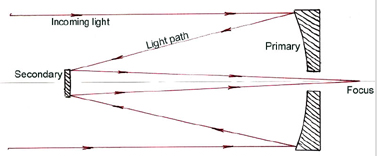
\includegraphics{cassegrain.png}
    \caption{Diagram showing the optical arrangement of the Cassegrain.}
    \label{cassegrain}
\end{figure}
The image will not necessarily be a perfect image: all rays regardless of
height $y$ at the surface (``surface'' refers to the lens or mirror), might not
cross at the same point. This is the subject of \textit{aberrations} (see
\S{}~{\ref{ab}}). For a ``smooth'' surface, the amount of aberration will
depend on how much the different rays differ in $y$, which depends on the shape
of the surface:
\begin{description}
    \item [paraxial rays] are near the center of the aperture.
    \item [marginal rays] are on the edge of the aperture.
    \item [chief ray] passes through the center of the aperture.
\end{description}
To define nominal (unaberrated) quantities, we consider the \textit{paraxial
regime}, a small region near the optical axis surrounding the chief ray. In
this regime, all angles are small, aberrations vanish (everything converges to
a point), and a surface can be wholly specified by its radius of curvature, $R$
(where the image is at the center of a ``circle'' with radius $R$).

The \textit{field angle} is formed when receiving light off-axis by some
angular amount. It is not necessarily zero in the paraxial regime.

For the time being, we are ignoring \textit{diffraction} and considering
\textit{geometric} optics, where spatial scales are much larger than the
wavelength ($x > \sim\lambda$).

The basic relation between the object location at $s$ and the image location at
$s'$ can be derived as a function of a surface where the index of refraction
changes (Schroeder, chapter 2).
\[
    \frac{n'}{s'}-\frac{n}{s} = \frac{(n'-n)}{R}
    \]
where $n$ and $n'$ are the index of refraction where the light is coming from
and in the lens, respectively. The points at $s$ and $s'$ are called
\emph{conjugate} (if one is known, the other can be calculated). If either $s$
or $s'$ is at infinity (true for astronomical sources at $s$), the other
distance is defined as the \emph{focal length}, $f$, of the optical element,
and is where the light is focused. For $s=\infty$, $f=s'$.

The quantity on the right side of the equation, which depends only on the
surface parameters (not the image or object locations), is defined as the
\emph{power}, $P$, of the surface:
\[
     P \equiv \frac{(n'-n)}{R} = \frac{n'}{f'} = \frac{n}{f}
    \]
A similar derivation can be made for the case of reflection:
\[
     \frac{1}{s'} + \frac{1}{s} = \frac{2}{R}
    \]
This shows that $f = R/2$ for a mirror.

The same result is obtained when considering reflection as
refraction with
$n' = -n$ (same amplitude, opposite sign):
\[
  \frac{n'}{s'}+\frac{n'}{s} = \frac{(n'+n')}{R}
\]

The \emph{focal ratio} (or \emph{F-number}) is defined as
\[
    f/ = \frac{f}{A}
    \]
where $A$ is the aperture diameter and $f/$ denotes the focal ratio.
For example, a 3.5-m telescope with a focal ratio of $f /10$
has a focal length of 35 meters.
The focal ratio gives the beam ``width''; systems with a small focal ratio
have a short focal length compared with $A$, and hence the imcoming
beam to the image is wide. Systems with small focal ratios are called
``fast'' systems; systems with large focal ratios are called ``slow'' systems.

\rule{\textwidth}{0.4pt}

{\small\hfill\textcolor{date}{Wednesday, March 2}}

The \emph{magnification} of a system gives the ratio of the image height to
the object height:
\[
    \frac{h'}{h} = \frac{s'-R}{s-R} = \frac{ns'}{n's}
    \]
The magnification is negative for both inverted images and for
reflection ($n' = -n$).
Magnification is an important quantity for \emph{multi-element} systems
(see \S{}~\ref{?}).

The \emph{plate scale} is defined as the
``motion'' of an image for given beam from infinity.
From a consideration of the chief rays
for objects on-axis and at field angle $\alpha$: {$$
    \tan{\alpha} \approx \alpha = \frac{x}{f}
$$} or {$$
    \textrm{scale} \equiv \frac{\alpha}{x} = \frac{1}{f}
$$}In other words, the scale, in units of angular motion (arcsec)
per physical motion in the focal plane ($x$), is given by $1/f$
(\textcolor{red}{important!})
For a fixed aperture
diameter, systems with a small $f/$ (smaller $f$) have
a \emph{larger} scale, i.e.\ more light in a patch of fixed physical size.
These are ``faster'' systems.

Example:
$\alpha = \frac{1}{35m} = \frac{1}{35\times10^{3}} = 2.86\times10^{-5}$
radians $ = 5.98''$/mm (there are 206265 arcseconds per radian).

\subsection{Multi-surface systems}
To combine surfaces, the image from the first surface becomes the
source for the second surface, and so on for each surface in the system.
The basic parameters of multi-surface systems can generally be described by
equivalent single-surface parameters.
For example, the \emph{effective} focal length
(the focal length of the first element multiplied by the magnification of
each subsequent element) of a multi-surface system
can be defined as the focal length of some
equivalent single-surface system.
The two systems (single and multi) are
equivalent in the paraxial approximation ONLY\@.

\subsubsection{A lens (has two surfaces)}
Consider a lens in air ($n \sim 1$). The first surface gives:{$$
    \frac{n}{s_{1}'}-\frac{1}{s_{1}} = \frac{n-1}{R_{1}}=P_{1}
$$}The second surface gives:{$$
    \frac{1}{s_{2}'}-\frac{n}{s_{2}} = \frac{n-1}{R_{2}}=P_{2}
$$}but we have $s_{2} = s_{1}'-d$ (remember we have to use the plane of the
second surface to measure distances for the second surface).

The effective focal length from the center of the lens
is given (after some algebra) by:{$$
    P=\frac{1}{f'}=P_{1}+P_{2}-\frac{d}{n}P_{1}P_{2} $$ $$
    P=\frac{(n-1)}{R_{1}}+\frac{(1-n)}{R_{2}}-\frac{d}{n}
    \frac{(n-1)(1-n)}{R_{1}R_{2}}
$$}From this, we derive the \emph{thin lens} formula:{$$
    P=\frac{1}{f'} = \frac{(n-1)}{R_{1}}+\frac{(1-n)}{R_{2}} =
    (n-1)\left( \frac{1}{R_1} - \frac{1}{R_2}\right)  $$ $$
    \frac{1}{f'} = \frac{1}{f_{1}} + \frac{1}{f_{2}}
$$}
\subsubsection{plane-parallel plate}
Zero power, but moves image laterally:{$$
    \Delta = d\left[1-\left(\frac{1}{n}\right)\right]
$$}Application to filters: variation of focus. If the focal length
changes, the scale changes; need to be careful when changing filters.
The focus may need to be shifted a bit. The filter width doesn't matter
but the index of refraction does. Holographic grating.
\subsubsection{Two-mirror telescopes}
In astronomy, most telescopes are two-mirror telescopes of Newtonian,
Cassegrain, or Gregorian design. All 3 types have a concave primary.
The Newtonian has a flat secondary, the Cassegrain a convex secondary,
and the Gregorian a concave secondary. The Cassegrain is the most
common for research; it is more compact than a Gregorian and
allows for magnification by the secondary. Basic parameters are
outlined \href{%
http://astronomy.nmsu.edu/holtz/a535/html/diagrams/a535/cassegra.htm}{%
    \textcolor{blue}{here}}.
Each of these telescope types defines a \emph{family} of
telescopes with different first-order performances. From the
usage/instrumentation point of view, important quantities are:
\begin{itemize}
    \item the diameter of the primary, which defines the light
        collecting power
    \item the scale of the telescope, which is related to the focal
        length of the primary and the magnification of the secondary:{$$
            f_{\textrm{eff}} = f_{1}m
        $$}(alternatively, the focal ratio of the telescope, which gives
        the effective focal length with the diameter)
    \item the back focal distance, which is the distance of the focal
        plane behind the telescope.
\end{itemize}
From the design point of view, we need to specify:
\begin{itemize}
    \item the radii of curvature of the mirrors
    \item the separation between the mirrors
\end{itemize}
The relation between the usage and design parameters can be derived
from simple geometry. Some basic definitions:
\begin{itemize}
    \item ratio of focal lengths, $\rho$:
        $$ \rho = \frac{R_2}{R_1} = \frac{f_2}{f_1}  $$
    \item magnification of the secondary, $m$ (be aware that $s_{2}'$ is
        \emph{negative} for a Cassegrain):
        $$ m = -\frac{s_2'}{s_2} $$
    \item \emph{back focal distance},
        the distance from the primary vertex to
        the focal plane (often expressed in units of the primary focal
        length, or primary diameter):
        $$ f_{1}\beta = D\eta  $$
    \item primary focal ratio, $F_{1}$:
        $$ F_{1} = \frac{f_{1}}{D} $$
    \item ratio of marginal ray heights, $k$:
        $$ k = \frac{y_{2}}{y_{1}}  $$
\end{itemize}
Using some geometry, some basic relations between these quantities
can be derived, in particular:{$$
    \rho = \frac{mk}{(m-1)}
$$}and{$$
    (1+\beta) = k(m+1)
$$}$\beta$ in units of primary mirror focal length.
Usually, $f_{1}$ is limited by technology/cost, in which case
$m$ can be chosen to match the
desired scale. $k$ is directly related to separation of mirrors, and is a
compromise between a shorter telescope and blocking out more
light vs.\ a longer telescope and blocking less light.
In either case, the focal plane has to be kept behind the primary.

\textcolor{myBlue}{%
Want telescope to match detector: how many arcseconds per pixel?
Straightforward in paraxial regime. Need to tune magnification of secondary.
How far apart do the mirrors need to be\ldots}

One final thing to note is how to focus a Cassegrain telescope. Most
instruments are placed at a fixed location behind the primary.
Ideally, this will be at the back focal distance, and everything
should be set as designed. However, sometimes the instrument may not
be exactly at the correct back focal distance, or it might move
slightly because of thermal expansion/contraction. In this case,
focussing is usually then done by moving the secondary mirror
(not the detector).

The amount of image motion for a given secondary motion is given by:{$$
    \frac{\textrm{d}\beta}{\textrm{d}k} =
    \frac{\textrm{d}}{\textrm{d}k}k\left(m+1\right)-1
$$}Working through the relations above, this gives:{$$
    \frac{\textrm{d}\beta}{\textrm{d}k} = m^{2}+1
$$}where $m^{2}$ is the magnification of the secondary mirror.
So the amount of focal plane motion ($f_{1}\textrm{d}\beta$)
for a given amount of secondary motion ($f_{1}dk$) depends on the
magnification of the system.

If the secondary is moved, $k$ is changed. Since $\rho$ is fixed by the
mirror shapes, the magnification can be changed as the secondary is
moved. This is expected since the system focal length is being changed:
$f = mf_{1}$. So it's possible that a given
instrument could have a slightly varying scale if its position is not
perfectly fixed relative to the primary.
Alternatively, if you need to independently focus and set the scale
(SDSS for example), then two things need to be moved.

Note that even if the instrument is right at the back focal
distance, movement of the secondary is required to account for
mechanical changing of spacing between the primary and secondary as a
result of thermal expansion/contraction.

\rule{\textwidth}{0.4pt}

{\small\hfill\emph{Monday, March 7, 2016}}
\subsubsection{Definitions for multi-surface system: stops and pupils}
\begin{itemize}
    \item aperture stop: determines the amount of light reaching an
        image (usually the primary mirror).
    \item field stop: determines the angular size of the field. This
        is usually the detector, but for a large enough detector, it
        could be the secondary.
    \item pupil: location where rays from all field angles fill the
        same aperture. Image of the primary mirror (not formed by
        the primary mirror). Number of elements in system = number
        of pupils.
    \item entrance pupil: image of aperture stop as seen from source
        object (usually the primary).
    \item exit pupil: image of aperture stop formed by all subsequent
        optical elements.
\end{itemize}
Stops are relevent for correcting aberrations.
In a two-mirror telescope, the location of the exit pupil is where the
image of the primary is formed by the secondary. This can be calculated
using $s=d$ as the object distance (where $d$ is the separation of the
mirrors), then with the reflection equation, we can solve for $s'$
which gives the location of the exit pupil relative to the secondary
mirror. If one defines the quantity $\delta$, such that $f_{1}\delta$
is the distance between the exit pupil and the focal plane,
then (algebra not shown):{$$
    \delta = \frac{m^{2}k}{m+k-1} = \frac{m^{2}(1+\beta)}{m^{2}+\beta}
$$}This pupil is generally not accessible, so access to a pupil is
needed, additional optics are used.

The exit pupil is an important concept. For aberrations, it is
the total wavefront error at the exit pupil which gives the system aberration.
Pupils are important for aberration compensation. They can also be used to
put light at a location that is independent of pointing errors.

\subsection{Aberrations}\label{ab}
\subsubsection{Surface requirements for unaberrated images}
Next consider \emph{non}-paraxial rays. The surface
required to make an unaberrated image can be derived using
\emph{Fermat's principle}, which
states that light travels in the path such that infinitesimally small
variations in the path doesn't change the travel time to first order:
$\textrm{d}t/\textrm{d}l$
is a minimum.
For a single surface, this reduces to
the statement that light travels the path which takes the least time.
An alternate way of stating Fermat's principle is that the \emph{optical path
length} (OPL) is unchanged to first order for a small change in path. The OPL
is given by:{$$
    OPL = \int{c\textrm{d}t} =
    \int{\frac{c}{v}v\textrm{d}t} =
    \int{n\textrm{d}s}
$$}Fermat's principle has a physical interpretation when one considers the
wave nature of light. It is clear that around a stationary point of the
optical path light, the maximum amount of light can be accumulated over
different paths with a minimum of destructive interference. By the wave
theory, light travels over all possible paths, but the light coming over
the ``wrong'' paths destructively interferes, and only the light coming over
the ``right'' path constructively interferes.

Fermat's principle can be used to derive the basic laws of reflection
and refraction (Snell's law).

Consider a perfect imaging system that takes all rays from an object
and converges them to an image. Since Fermat's principle says
the only paths taken will be those for which the OPL is minimally changed
for small changes in path, the only way a perfect image will be formed is
when all optical path lengths along a surface between an image and object
point are the same - otherwise the light doesn't get to this point.

Instead of using Fermat's principle, we could solve for the parameters
of a perfect surface using analytic geometry, but this would require an
inspired guess for the correct functional form of the surface.

The perfect surface depends on whether the
light comes from a source at finite or infinite distance, and whether
the mirror is concave or convex.
The z-axis is the optical axis, perpendicular to the y-axis.
The goal is to figure out the shape of the surface, $y(z)$, that gives
a perfect image.

\textbf{\emph{%
Concave mirror with one conjugate at infinity: Parabola}}
\par Sample application: primary mirror of telescope looking at stars.
Fermat's principle gives:{$$
    y^{2} = 2R_{z}
$$}where $R = 2f$, the radius of curvature at the mirror vertex.
Note, however, that a prabola makes a perfect image
only for \emph{on}-axis images (field angle = 0), which is why we don't always
use this shape.

\textbf{\emph{%
Concave mirror with both conjugates at finite distances: Ellipse}}
\par Sample application: Gregorian secondary looking at image formed by primary.
Again, this is perfect only for field angle = 0.{$$
    \frac{(z-a)^{2}}{a^{2}} + \frac{y^{2}}{b^{2}} = 1 $$ $$
    y^{2} - \frac{2zb^{2}}{a} + \frac{z^{2}b^{2}}{a^{2}} = 0
$$}where{$$
    a = \frac{s+s'}{2} $$ $$
    b = \sqrt{(ss')} $$ $$
    R = \frac{ss'}{s+s'} = \frac{2b^{2}}{a}
$$}
\textbf{\emph{%
Convex mirror with both conjugates at finite distance: Hyperbola}}
\par Sample application: Cassegrain secondary looking at
image formed by primary:{$$
    \frac{(z-a)^{2}}{a^{2}} - \frac{y^{2}}{b^{2}} = 1 $$ $$
    y^{2} + \frac{2zb^{2}}{a} - \frac{z^{2}b^{2}}{a^{2}} = 0
$$}where{$$
    a = \frac{s+s'}{2} $$ $$
    b^{2} = \sqrt{(-ss')}
$$}($s$ is negative){$$
    R = -\frac{2b^{2}}{a}
$$}Let secondary ``relax'' to get perfect image. Most telescopes adjust
both surfaces, which allows for more freedom to get perfect images on
and off-axis.
\textbf{\emph{%
Convex mirror with one conjugate at infinity: Parabola}}
\par\ldots but this has no astronomical applications.

\textbf{\emph{2D to 3D}}
\par So far all cases have considered a one-dimensional surface.
Generalize to 2D surfaces by rotating around the z-axis.
For the equations, simply replace $y^{2}$ with $(x^{2} + y^{2})$.

\textbf{\emph{Conic sections}}
\par All of these figures are
\emph{conic sections}, described by a single equation:{$$
    \rho^{2} - 2Rz + (1+K)z^{2} = 0
$$}where $ \rho^{2} = x^{2} + y^{2} $
and $R$ is the radius of curvature at the mirror vertex,
$K$ is called the conic constant ($K = -e^{2}$, where $e$ is the eccentricity for
an ellipse, $e(b, a)$).
\begin{description}
    \item [$K > 0$] prolate ellipsoid
    \item [$K = 0$] sphere
    \item [$-1 < K < 0$] oblate ellipsoid
    \item [$K = - 1$] paraboloid
    \item [$K < - 1$] hyperboloid
\end{description}

\rule{\textwidth}{0.4pt}

\subsubsection{Aberrations: general description and low-order aberrations}

{\small\hfill\emph{Wednesday, March 23}}

Now consider what happens for surfaces that are \emph{not} perfect, e.g.\ for
a field angle $\neq$ 0 in the cases discussed above
(since only a sphere is symmetric for all field angles),
or for field angle $=$ 0 for a conic
surface that doesn't give a perfect image.

This is where \emph{aberrations} arise;
the light from all locations in the aperture
does not land at any common point.

Aberrations can be considered in either of two ways:
\begin{itemize}
    \item All rays don't land at a common point.
    \item Wavefront deviates from a spherical wavefront.
\end{itemize}
These two descriptions are equivalent. The former refers to
\emph{transverse} aberrations (the distance by which the
rays miss the paraxial focus), or \emph{angular} aberrations
(the angle by which the rays deviate from the perfect ray which will hit
paraxial focus). The latter refers to the wavefront error
(the deviation of the wavefront from a spherical wavefront as a
function of location in the exit pupil).

In general, the angular and transverse aberrations can be determined
from the optical path difference between a given ray and that of a
spherical wavefront. The relations are given by:{$$
    \textrm{angular aberration} =
    \frac{\textrm{d}\left(2\Delta{z}\right)}{\textrm{d}\rho}$$ $$
    \textrm{transverse aberration} =
    s'\frac{\textrm{d}\left(\Delta{z}\right)}{\textrm{d}\rho}
$$}$s'$ is the focal length.
If the aberrations are not symmetric in the pupil, then
define angular and transverse $x$ and $y$ aberrations separately by taking
derivatives with respect to $x$ or $y$ instead of $\rho$.

\textbf{\emph{Spherical aberration}}
\par First, consider the axisymmetric case of looking at an object on axis
(field angle $=$ zero) with an optical element that is a conic
section. Consider where rays land as $f(\rho)$, and derive
the effective focal length, $f_{e}(\rho)$, for an arbitrary conic
section [figure here]:{$$
    z_0 = \frac{\rho}{\tan(2\phi)} = \frac{\rho(1-(\tan\phi)^{2})}{2\tan\phi}$$ $$
    \tan\phi = \frac{\textrm{d}z}{\textrm{d}\rho}
$$}from the conic equation:{$$
    \rho^{2} - 2Rz + (1+K)z^{2} = 0 $$ $$
    z = \frac{R}{(1+K)}\left[1-\left(1-\frac{\rho^{2}}{R^{2}}
    \left(1+K\right)\right)^{1/2}\right] $$ $$
    z \approx \frac{\rho^{2}}{2R}+(1+K)\frac{\rho^{4}}{8R^{3}} +
    (1+K)^{2}\frac{\rho^{6}}{16R^{5}} + \ldots $$ $$
    \frac{\textrm{d}z}{\textrm{d}\rho} =
    \frac{\rho}{\left(R-\left(1-K\right)z\right)} $$ $$
    z_{0} = \frac{\rho}{2}
    \left[\frac{R-(1+K)z}{\rho} - \frac{\rho}{R-(1+K)z}\right] $$ $$
    f_{e} = z + z_{0} $$ $$
    f_{e} = \frac{R}{2} + \frac{(1-K)z}{2} - \frac{\rho^{2}}{2(R-(1+K)z)}$$ $$
    f_{e} = \frac{R}{2} - (1+K)\frac{\rho^{2}}{4R} - (1+K)(3+K)\frac{\rho^{4}}{16R^{3}} - \ldots $$ $$
    \Delta{f} = f_{e} - \frac{R}{2}
$$}
Note that $f_{e}$ is independent of $z$ only for $K=-1$, a parabola.
Also note that $\Delta{f}$ is symmetric with respect to $\rho$.
\textcolor{myBlue}{%
    $R/2$: paraxial focus. Spherical aberration is different from
    focusing\ldots can't just move focal plane around to get a perfect image.
    Where's the best place to focus to minimize aberrations?
    ``Circle of least confusion''. Deviations are symmetric in pupil,
    but not symmetric for focal position. Can solve TSA equations for
    conic section equations.
}

Spherical aberration is defined as the aberration resulting from
$K\neq-1$ ($K+1 = 0$ for parabola).
Rays from different radial positions in the entrance
aperture focus at different locations. It is an aberration which is
present on axis as seen \href{%
http://astronomy.nmsu.edu/holtz/a535/html/diagrams/a535/spher.htm}
{\textcolor{blue}{here}}. Spherical aberration is symmetric in
the pupil. There is no location in space where all rays focus at a
point. Note that the behavior (image size) as a function of focal
position is not symmetric. One can define several criteria for where
the ``best focus'' might be, leading to the terminology paraxial
focus, marginal focus, diffraction focus, and the circle of least
confusion.

The asymmetric nature of spherical aberration as a function of focal
position distinguishes it from other aberrations and is a useful
diagnostic for whether a system has this aberration. This is shown in this
\href{http://astronomy.nmsu.edu/holtz/a535/html/diagrams/a535/z11.htm}
{\textcolor{blue}{figure}} which shows a sequence of images at different focal
positions in the presence of spherical aberration.
A \emph{transverse spherical aberration} (TSA) is the image size at paraxial
focus. This is not the location of the minimum image size.\\
(figure here){$$
    \frac{\textrm{TSA}}{\Delta{f}} = \frac{\rho}{f-z(\rho)} $$ $$
    \textrm{TSA} = -(1+K)\frac{\rho^{3}}{2R^{2}} -
    3(1+K)(3+K)\frac{\rho^{5}}{8R^{4}} + \ldots
$$}The difference in angle between the ``perfect'' ray from the parabola
and the actual ray is called the \emph{angular aberration}, in this case
\emph{angular spherical aberration} (ASA).\\
(figure here){$$
    \textrm{ASA} = 2(\phi_{P}-\phi) \approx
    \frac{\textrm{d}}{\textrm{d}\rho}(2\Delta{z}) \approx
    -(1+K)\frac{\rho^{3}}{R^{3}}
$$}where $2\Delta{z}$ gives the optical path difference between the two rays.

This is simply related to the transverse aberration:{$$
    \textrm{TSA} = \frac{R}{2}\textrm{ASA}
$$}We can also consider aberration as the difference between our
wavefront and a spherical wavefront, which in this case is the
wavefront given by a parabolic surface.\\
(figure here){$$
    \Delta{z} = z_{\textrm{parabola}}-z\left(K\right) =
    -\frac{\rho^{4}}{8R^{3}}\left(1+K\right) + \ldots
$$}
\textcolor{red}{More stuff here, but pretty sure it's a repeat.}

\textbf{\emph{General aberration description}}
\par\textcolor{myBlue}{%
    Surface described by polynomial, optical path difference, low
    order\ldots something, OPD (last term doesn't have field angle
    dependence). Restrict to third-order aberrations (fourth order
    in OPD). Order of pupil backed down by 1. $\theta$ - ``amount off
    axis that you go''. (Reveiw ``order'' for maths). $\theta^{2}y$ -
    $\theta$ is squared so direction doesn't matter (astigmatism),
    $\theta$ - coma (linear), $y\rho^{2}$ - spherical aberration
    (no $\theta$).
}
\par We can describe deviations from a spherical wavefront generally. Since
all we care about are optical path differences, we write an expression
for the optical path difference between an arbitrary ray and the chief
ray, and in doing this, we can also include the possibility of an
off-axis image, and get{$$
    OPD = OPL - OPL(chiefray) $$ $$
    OPD = A_0y + A_1y^{2} + A_1'x^{2} + A_2y^{3} + A_2'x^{2}y + A_3\rho^{4}
$$}where we've kept terms only to fourth order and chosen our coordinate
system such that the object lies in the y-z plane. The coefficients,
$A$, depend on lots of things, such as ($\theta, K, n, R, s, s'$).

Note that rays along the y-axis are called \emph{tangential} rays,
while rays along the x-axis are called \emph{sagittal} rays.

Analytically, generally restricted to
\emph{third-order} aberrations, which are fourth-order
(in powers of $x, y, \rho$, or $\theta$) in the optical path
difference, because of the derivative we take to get transverse or
angular aberrations. In the third-order limit,
$A2 = A2'$, and $A1 = -A1'$. Working
out the geometry, we find for a mirror that:{$$
    A_{0} = 0 $$$$
    A_{1} = \frac{n\theta^{2}}{R}$$$$
    A_{2} = -\frac{n\theta}{R^{2}}\left(\frac{m+1}{m-1}\right)$$$$
    A_{3} = \frac{n}{4R^{3}}\left[K+\left(\frac{m+1}{m-1}\right)^{2}\right]
$$}
From the general expression, we can derive the angular or the
transverse aberrations in either the $x$ or $y$ direction. Considering the
aberrations in the two separate directions, we find:{$$
    AA_y = 2A_1y + A_2(x^{2}+3y^{2}) + 4A_3y\rho^{2}  $$$$
    AA_x = 2A_1'x + 2A_2xy + 4A_3x\rho^{2}
$$}The first term is proportional to $\theta^{2}y$ and is called
\emph{astigmatism}. The second term is proportional to
$ \theta(x^{2} +3y^{2})$
and is called \emph{coma}. The final term, proportional to
$y\rho^{2}$
is \emph{spherical aberration}, which we've already discussed (note for
spherical, $AA_x = AA_y$ and in fact the $AA$ in any direction is equal,
hence the aberration is circularly symmetric).

\textbf{\emph{Astigmatism}}
\par For astigmatism, rays from opposite sides of the pupil focus in
different locations relative to the paraxial rays. At the paraxial
focus, we end up with a circular image. As you move away from this
image location, you move towards the tangential focus in one
direction and the sagittal focus in the other direction. At either of
these locations, the astigmatic image looks like a elongated ellipse.
Astigmatism goes as $\theta^{2}$, and consequently looks the same
for opposite field angles. Astigmatism is characterized in the image
plane by the \emph{transverse} or \emph{angular} astigmatism (TAS or AAS), which
refer to the height of the marginal rays at the paraxial focus.
Astigmatism is symmetric around zero field angle.
\textcolor{myBlue}{%
    elliptical shape $\rightarrow$ circle $\rightarrow$ ellipse again.
    Need to consider tangential rays and sagittal rays. ``Useful'':
    look for where T changes to S.
}
This \href{http://astronomy.nmsu.edu/holtz/a535/html/diagrams/a535/astig.htm}
{\textcolor{blue}{figure}} shows the rays in the presence of astigmatism.
This \href{http://astronomy.nmsu.edu/holtz/a535/html/diagrams/a535/z5.htm}
{\textcolor{blue}{figure}}
shows the behavior of astigmatism as one passes through paraxial focus.

\textbf{\emph{Coma}}

\textcolor{myBlue}{%
    Looks like a comet! Same distance from pupil, not same distance
    from focal plane. Can't tell which side of (?) you're on.
}
For coma, rays from opposite sides of the pupil focus at the same
focal distance. However, the tangential rays focus at a different
location than the sagittal rays, and neither of these focus at the
paraxial focus. The net effect is to make an image that vaguely looks
like a comet, hence the name coma. Coma goes as $\theta$, so the
direction of the comet flips sign for opposite field angles. Coma is
characterized by either the \emph{tangential} or \emph{sagittal
transverse/angular coma} (TTC, TSC, ATC, ASC) which describe the
height/angle of either the tangential or sagittal marginal rays at the
paraxial focus: $TTC = 3TSC$.

This \href{http://astronomy.nmsu.edu/holtz/a535/html/diagrams/a535/coma.htm}
{\textcolor{blue}{figure}} shows the rays in the presence of coma.
This \href{http://astronomy.nmsu.edu/holtz/a535/html/diagrams/a535/z7.htm}
{\textcolor{blue}{figure}} shows the behavior of coma as one passes
through paraxial focus.
In fact, there are two more third-order aberrations:
\textit{distortion} and \textit{field curvature},
\mynotes{``field flattener''}.
Neither affects image quality, only location;
\mynotes{the images go off-axis} (unless
you are forced to use a flat image plane). Field curvature gives a
curved focal plane: if imaging onto a flat detector, this will lead to
focus deviations as one goes off-axis. Distortion affects the location
of images in the focal plance, and goes as $\theta^{3}$.
The amount of field curvature and distortion can be derived from the
aberration coefficients and the mirror parameters.

We can also determine the relevant coefficients for a surface with a
displaced stop (Schroeder p 77), or for a surface with a decentered
pupil (Schroeder p89-90); it's just more geometry and algebra. With
all these realtions, we can determine the optical path differences for
an entire system: for a multi-surface system, we just add the OPD's as
we go from surface to surface. The final aberrations can be determined
from the system OPD.

\rule{\textwidth}{0.4pt}

{\small\hfill\emph{Wednesday, March 30}}

\subsubsection{Aberration compensation and different telescope types}

Using the techniques above, we can write expressions for the system
aberrations as a function of the surface figures (and field angles).
If we give ourselves the freedom to choose surface figures, we can
eliminate one (or more) aberrations.

For example, given a conic constant of the primary mirror, we can use
the aberration relations to determine $K_2$ such that spherical
aberration is zero; this will give us perfect images on-axis. We find
that:{$$
    K_2 = \left(\frac{m+1}{m-1}\right)^{2} +
    \frac{m^{3}}{k\left(m-1\right)^{3}}\left(K_{1}+1\right)
$$}satisfies this criterion.  If we set the primary to be a parabola
($K_{1} = -1$), this gives the conic constant of the secondary we must use to
avoid spherical aberration. This type of telescope is called a
\emph{classical} telescope. Using the aberration relations, we can determine
the amount of astigmatism and coma for such telescopes, and we find
that coma gives significantly larger aberrations than astigmatism.

If we allow ourselves the freedom to choose both $K_1$ and $K_2$,
we can eliminate both spherical aberration and coma.
Designs of this sort are called \emph{aplanatic}.
The relevant expression, in terms of the magnification and
back focal distance (we could use the relations discussed earlier to
present these in terms of other paraxial parameters), is:{$$
    K_{1} = -1 - \frac{2(1+\beta)}{m^{2}(m-\beta)}
$$}We can only eliminate two aberrations with two mirrors, so even this
telescope will be left with astigmatism.

There are two different classes of two-mirror telescopes that allow
for freedom in the shape of both mirrors: Cassegrain telescopes and
Gregorian telescopes (Newtonians have a flat secondary). For the
classical telescope with a parabolic primary, the Cassegrain
secondary is hyperbolic, whereas for a Gregorian it is ellipsoidal
(because of the appropriate conic sections derived above for convex
and concave mirrors with finite conjugates). For the aplanatic
design, the Cassegrain telescope has two hyperbolic mirrors, while
the Gregorian telescope has two ellipsoidal mirrors. An aplanatic
Cassegrain telescope is called a \emph{Ritchey-Chretien} telescope.

The following table gives some characteristics of ``typical''
telescopes. Aberrations are given at a field angle of 18 arc-min in
units of arc-seconds. Coma is given in terms of tangential coma.

\begin{table}[h]
\centering
\begin{tabular}{c r r r r}
Parameter & CC & CG & RC & AG\\
\hline\hline
m & 4.00 & -4.00 & 4.00 & -4.00\\
k & 0.25 & -0.417 & 0.25 & -0.417\\
1-k & 0.75 & 1.417 & 0.75 & 1.417\\
mk & 1.000 & 1.667 & 1.000 & 1.667\\
ATC & 2.03 & 2.03 & 0.00 & 0.00\\
AAS & 0.92 & 0.92 & 1.03 & 0.80\\
ADI & 0.079 & 0.061 & 0.075 & 0.056\\
$\kappa_{m}R_{1}$ & 7.25 & -4.75 & 7.625 & -5.175\\
$\kappa_{P}R_{1}$ & 4.00 & -8.00 & 4.00 & -8.00\\
\hline
\end{tabular}
\caption{Characteristics of Two-Mirror Telescopes}
\end{table}

The image quality is clearly better for the aplanatic designs than for
the classical designs, as expected because coma dominates off-axis in
the classical design. In the aplanatic design, the Gregorian is
slightly better. However, when considerations other than just optical
quality are considered, the Cassegrain usually is favored: for the
same primary mirror, the Cassegrain is considerably shorter and thus
it is less costly to build an enclosure and telescope structure. To
keep the physical length the same, the Gregorian would have to have a
faster primary mirror, which are more difficult (i.e.\ costly) to
fabricate, and which will result in a greater sensitivity to alignment
errors. Both types of telescopes have a \emph{curved} focal plane.

\subsection{Sources of aberrations}
So far, we have been discussing aberrations which arise from the
optical design of a system when we have a limited number of elements.
However, it is important to realize that aberrations can arise from
other sources as well. These other sources can give additional
third-order aberrations, as well as higher order aberrations. Some
possible sources include:
\begin{itemize}
    \item misfigured (a slightly harsh term)
        or imperfectly figured optics: rarely is an element made
        exactly to specification.
    \item misalignments. If the mirrors in a multiple-element system are not
        perfectly aligned, aberrations will result. The centers must be
        lined up. These can be derived
        (third-order) from the aberration expressions for decentered elements.
        For two mirror systems, decentering or tilting the
        secondary introduces a constant amount of coma over the field. Coma
        dominates astigmatism for a misaligned telescope.
        The Ritchey-Chretian has a ``high'' tolerance for this (not much
        wiggle room).
    \item mechanical/support problems. When the mirrors are mounted in mirror
        cells the weight of the mirror is distributed over some support
        structures. Because the mirrors are not infinitely stiff, some
        distortion of the mirror shape will occur. Generally, such distortion
        will probably change as a function of which way the telescope is
        pointing. Separate from this, becuase the telescope structure itself
        is not perfectly stiff, one expects some flexure which gives a
        different secondary (mis)alignment as a function of where one is
        pointing. Finally, one might expect the spacing between the primary
        and secondary to vary with temperature, if the telescope structure is
        made of materials which have non-zero coefficients of expansion.
    \item chromatic aberration. Generally, we've only been discussing mirrors
        since this is what is used in telescopes. However, astronomers often
        put additional optics (e.g., cameras or spectrographs) behind
        telescopes which may use refractive elements rather than mirrors.
        There are aberration relations for refractive elements just as we've
        discussed, but these have additional dependences on the indices of
        refraction of the optical elements. For most refractive elements, the
        index of refraction varies with wavelength, so one will get
        wavelength-dependent aberrations, called chromatic aberrations. These
        can be minimized by good choices of materials or by using combinations
        of different materials for different elements; however, it is an
        additional source of aberration.
    \item seeing. This is the only natural source of aberration (the one
        we can't control).
        The earth's atmosphere introduces optical path differences
        between the rays across the aperture of the telescope. This is
        generally the \textbf{dominant} source of image degradation from a ground-based
        telescope. Consequently, one builds telescopes in good sites, and as
        far as design and other sources of image degradation are concerned,
        one is generally only interested in getting these errors small when
        compared with the smallest expected seeing errors.
\end{itemize}

\subsection{Ray tracing}

For a fully general calculation of image quality, one does not wish
to be limited to third-order aberrations, nor does one often wish to
work out all of the relations for the complex set of aberrations
which result from all of the sources of aberration mentioned above.
Real world situations also have to deal with \emph{vignetting} in optical
systems, in which certain rays may be blocked by something and never
reach the image plane (e.g., in a two-mirror telescope, the central
rays are blocked by the secondary).

Because of these and other considerations, analysis of optical
systems is usually done using \emph{ray tracing}, in which the parameters of
an optical system are entered into a computer, and the computer
calculates the expected images on the basis of geometric optics. Many
programs exist with many features: one can produce \emph{spot} diagrams
which show the location of rays from across the aperture at an image
plane (or any other location), plots of transverse aberrations, plots
of optical path differences, etc. \texttt{zmacs} is a ray-tracing
program.

(Demo ray trace program. Start with on-axis object, single mirror.
Where is focus? What will image look like with spherical mirror? What
do we need to do to make it perfect? How does it depend on aperture
size? Now how do off-axis images look like? spot diagrams, through
focus, ray fan, opd plots, etc. Now introduce second mirror. What
determines where focus will be? Magnification? What shape to make a
perfect on-axis image? What do off-axis images look like? How do we
make them better? Now how is performance? Real 3.5m and 1m
prescriptions. Issue: guider.)

\subsection{Physical (diffraction) optics}

Up until now, we have avoided considering the wave nature of light
which introduces \textit{diffraction} from interference of light coming from
different parts of the aperture. Because of diffraction, images of a
point source will be slightly blurred. From simple geometric arguments,
we can estimate the size of the blur introduced from diffraction:
(figure here)

We find that:
\[
    \theta \sim \frac{\lambda}{D}
    \]
Using this, we find that the diffraction blur is smaller than the blur
introduced by seeing for $D > 0.2$ meters at 5500 \AA{}, even for the
excellent seeing conditions of 0.5 arcsecond images. However, the
study of diffraction has become important recently because of several
reasons: 1) the existence of the Hubble Space Telescope, which is
diffraction limited (no seeing), 2) the increasing use of infrared
observations, where diffraction is more important than in the optical,
and 3) the development of adaptive optics, which attempts to remove
some of the distortions caused by seeing. Consequently, it's now
worthwhile to understand some details about diffraction.

To work out in detail the shape of the images formed from diffraction
involves understanding wave propagation. Basically, one integrates
over all of the source points in the aperture (or exit pupil for an
optical system), determining the contribution of each point at each
place in the image plane. The contributions are all summed taking into
account phase differences at each image point, which causes
reinforcment at some points and cancellation at others. The expression
which sums all of the individual source points is called the
\textit{diffraction integral}. When the details are worked out,
the intensity in the image plane is related to the intensity and phase
at the exit pupil. In fact the wavefront is described at any plane by
the \textit{optical transfer function}, which gives the intensity and phase of
the wave at all locations in that plane. The OTF at the pupil plane
and at the image plane are a Fourier transform pair. Consequently, we
can determine the light distribution in the image plane by taking the
Fourier transform of the pupil plane; the light distribution, or point
spread function, is just the modulus-squared of the OTF at the image
plane. Symbolically, we have
\[
    PSF = \left\vert{FT(OTF(pupil))}\right\vert^{2}
    \]
where $FT$ represents a Fourier transform, and
\[
    OTF(pupil) = P(x,y)e^{ik\phi(x,y)}
    \]
$P(x,y)$ is the \textit{pupil function}, which gives the transmission
properties of the pupil, and usually consists of ones and zeros for
locations where light is either transmitted or blocked (e.g., for a
circular lens, the pupil function is unity within the radius of lens,
and zero outside; for a typical telescope the pupil function includes
obscuration by the secondary and secondary support structure).
$\phi$ is the phase in the pupil. More relevantly, $\phi$ can be
taken to be the optical path difference in the pupil with some
fiducial phase, since only OPDs matter, not the absolute phase.
Finally the wavenumber $k$ is just $\frac{2\pi}{\lambda}$.

For the simple case of a plane wave with \textbf{no phase errors}, the
diffraction integral can be solved analytically. The result for a
circular aperture with a central obscuration, when the fractional
radius of the obscuration is given by $\epsilon$, the expression for
the PSF is:
\[
    PSF \propto \left[
        \frac{2J_{1}(v)}{v} -
        \epsilon^{2}\frac{2J_{1}(\epsilon{v})}{\epsilon{v}}
        \right]^{2}
    \]
\[
    v = \frac{\pi{r}}{\lambda{F}}
    \]
where $J_{1}$ is a first order Bessel function, $r$ is the distance in the
image plane, $\lambda$ is the wavelength, and $F$ is the focal ratio
($F=f/D$).

This expression gives the so-called \textit{Airy pattern} (the solution?)
which has a central disk surrounded by concentric dark and bright rings.
The radius of the first dark ring is at the physical distance
$r = 1.22\lambda F$, or alternatively, the angular distance
$\theta = 1.22\lambda/D$. This gives the size of the \textit{Airy disk}.
\mynotes{For the APO 3.5 m, $\theta \sim 0.02''$, but we get $\sim 1''$
because we're \textit{seeing dominated}.}

For more \textbf{complex cases}, the diffraction integral is solved
numerically by doing a \textit{Fourier transform}. The pupil function is often
more complex than a simple circle, because of additional
items which block light in the pupil, such as the support structures
for the secondary mirror.

This \href{http://astronomy.nmsu.edu/holtz/a535/html/diagrams/a535/airy.htm}
{figure} shows the Airy pattern, both without obscurations,
and with a central obscuration and spiders in a setup typical of a telescope.

In addition, there may be \textit{phase errors} in the exit pupil, because of
the existence of any one of the sources of aberration discussed
above. For general use, $\phi$ is often expressed as an series,
where the expansion is over a set of orthogonal polynomials for the
aperture which is being used. For circular apertures with (or
without) a central obscuration (the case most often found in
astronomy), the appropriate polynomials are called \textit{Zernike}
polynomials. The lowest order terms are just uniform slopes of phase
across the pupil, called tilt, and simply correspond to motion in the
image plane. The next terms correspond to the expressions for the OPD
which we found above for focus, astigmatism, coma, and spherical
aberration, generalized to allow any orientation of the phase errors
in the pupil. Higher order terms correspond to higher order
aberrations. \mynotes{Zernike polynomials: expansion, each tilted in
different direction and/or parabolic}.

This \href{http://astronomy.nmsu.edu/holtz/a535/html/diagrams/a535/zernike.htm}
{figure} shows the form of some of the low order Zernike terms:
the first corresponds to focus aberration, the next two to
astigmatism, the next two to coma, the next two to trefoil
aberration, and the last to spherical aberration.

A wonderful example of the application of all of this stuff was in the
diagnosis of spherical aberration in the Hubble Space Telescope, which
has been corrected in subsequent instruments in the telescope, which
introduce spherical aberration of the opposite sign. To perform this
correction, however, required and accurate understanding of the
amplitude of the aberration. This was derived from analysis of
on-orbit images, as shown in this
\href{http://astronomy.nmsu.edu/holtz/a535/html/diagrams/a535/hstspher.htm}
{figure}.
Note that it is possible in
some cases to try to recover the phase errors from analysis of images.
This is called \textit{phase retrieval}. There are several ways of trying to do
this, some of which are complex, so we won't go into them, but it's
good to know that it is possible. But an accurate amplitude of
spherical aberration was derived from these images. This derived value
was later found to correspond almost exactly to the error expected
from an error which was made in the testing facility for the HST
primary mirror, and the agreement of these two values allowed the
construction of new corrective optics to proceed\ldots

\test{Understand the principles of diffraction optics and, in particular,
how diffraction scales with wavelength and aperture diameter. Know the
terminology: optical transfer function, pupil function, and how phase
errors across the pupil can be decomposed into a series of Zernike polynomials.}

\subsection{Adaptive optics}
\mydate{Monday, April 4}

\textbf{The goal of \textit{adaptive optics} is to partially or entirely remove
the effects of atmospheric seeing.} This is different from \textit{active}
optics, which works at lower frequencies ($\ll$ 1 Hz), whereas adaptive optics
must work at 10 to 1000 Hz.  At low frequencies, the active optics can be done
with actuators on the primary and secondary mirrors themselves.  At the high
frequencies reqiured for adaptive optics, however, these large mirrors cannot
respond fast enough, so it is required to form a pupil on a smaller mirror
which can be rapidly adjusted; hence adaptive optics systems are really
separate astronomical instruments.

\mynotes{Camera behind, make image of primary mirror.
Actuators ``push me pull you'' on back of mirror.
Image pupil and do corrections there (much smaller\ldots actual
primary mirror is too big).}

Many adaptive optics systems functioning and/or under development:
(lots of links here).

The basic idea of an adaptive optics system is to \textbf{rapidly sense the
wavefront errors and then correct for them on timescales faster
than those at which the atmosphere changes}. Consequently, there are
three parts to an adaptive optics system:
\begin{enumerate}
    \item A component that senses wavefront errors
    \item A control system that figures out how to correct these errors
    \item An optical element that receives the signals from the
        control system and implements wavefront corrections
\end{enumerate}
There are several methods used for wavefront sensing. Two that are in
fairly common use today are
\begin{enumerate}
    \item \href{%
        http://astronomy.nmsu.edu/holtz/a535/html/diagrams/a535/beckers3.htm}
        {Shack-Hartmann sensors}
    \item wavefront curvature sensing devices
\end{enumerate}
In a Shack-Hartmann sensor,
\mynotes{(determine wiggly wavefront; uses image of primary)}, an array of
lenslets \mynotes{(lots of little telescopes in exit pupil)}
is put in a pupil plane and each
lenslet images a small part of the pupil. Measuring image shifts between each
of the images gives a measure of the local wavefront tilts. Wavefront curvature
devices look at the intensity distribution in out-of focus images. Other
wavefront sensing techniques include pyramid wavefront sensors and phase
diversity techniques. Usually, a star is used as the source, but this is not
required for some wavefront sensors (in other words, an extended source can be
used).

To correct wavefront errors, a deformable mirror is used. These can be
generically split into two categories: segmented and continuous faceplate
mirrors, where the latter are more common. A deformable mirror is
characterized by the number of adjustable elements: the more elements there
are, the more correction can be done. LCD arrays have also been used for
wavefront correction.

In general, it is very difficult to achieve complete correction even for ideal
performance, and the effectiveness of different adaptive optics systems needs
to be considered.  This effectiveness depends on the size of the aperture, the
wavelength, the number of resolution elements on the deformable mirror, and the
quality of the site.  Clearly, more resolution elements are needed for larger
apertures.  Equivalently, the effectiveness of a system will decrease as the
aperture is increased for a fixed number of resolution elements.  The return
can be considered as a function of Zernike order corrected and aperture size.
(\mynotes{uh, do hwut?}) For large telescopes, you'll only get
partial correction unless a very large number of resolution elements on the
deformable mirror are available. The following table gives the mean square
amplitude, $\Delta_{j}$, for Kolmogorov turbulence after removal of the first
$j$ terms; the rms phase variation is just
$ \frac{\sqrt{\Delta_{j}}}{2\pi} $.

\mynotes{$\Delta_{j}$ - rms around wavefront error; comes down even
for lower order.}

For small apertures, you can make significant gains with removal of just low
order terms, but for large apertures you need very high order terms. Note
various criteria for quality of imaging, e.g.\ $\lambda/4$, etc.
\newpage
\begin{table}[th]
\centering
\begin{tabular}{c c c c c c c}
    $Z_j$ & $n$ & $m$ & Expression & Description &
    $\Delta_j$ & $\Delta_j - \Delta_{j-1}$\\
    \hline\hline
    Z1 & 0 & 0 & 1 & constant & 1.030 s & n/a\\
    Z2 & 1 & 1 & 1 & tilt & 1.030 s & n/a\\
    Z3 & 1 & 1 & 1 & tilt & 1.030 s & n/a\\
    Z4 & 2 & 1 & 1 & defocus & 1.030 s & n/a\\
    Z5 & 2 & 2 & 1 & astigmatism & 1.030 s & n/a\\
    Z6 & 2 & 2 & 1 & astigmatism & 1.030 s & n/a\\
    Z7 & 3 & 1 & 1 & coma & 1.030 s & n/a\\
    Z8 & 3 & 1 & 1 & coma & 1.030 s & n/a\\
    Z9 & 3 & 3 & 1 & trifoil & 1.030 s & n/a\\
    Z10 & 3 & 3 & 1 & trifoil & 1.030 s & n/a\\
    Z11 & 4 & 0 & 1 & spherical & 1.030 s & n/a\\
    \hline
    \end{tabular}
\end{table}
\begin{itemize}
    \item $r$ = distance from center circle
    \item $\phi$ = azimuth angle
    \item $S=(D/r_0)^{5/3}$ \mynotes{(from turbulence theory)}
\end{itemize}
\mynotes{Bigger $r_{0}$ is good (better seeing). NIR is best for
AO systems.}

Another important limitation is that an object on which you can derive the
wavefront is needed. Measurements of wavefront are subject to noise just like
any other photon detection, so bright sources may be required. This is even
more evident considering a source that is within the same isoplanatic patch as
the desired object is needed. Recall that the wavefront changes on time scales
of milliseconds. These requirements place limitations on the amount of sky over
which it is possible to get good corrections. It also places limitations on the
sorts of detectors that are needed in the wavefront sensors (fast readout and
little to no readout noise).

\mynotes{4/06/16 Another challenge: wavefront sensing. Need one subcell for
each $r_{0}$. How much light does each element collect? Not much\ldots
Exposure time needs to be short enough that atmosphere doesn't change during
that time. \underline{Isoplanatic patch}: same blurring pattern;
size scale: $\theta \sim$ arcsec - 1 arcmin.
Following table:
Typical $r_{0}$ values [cm] and typical timescales ($\tau_{0}$) [seconds].
$V_{lim}$ - subaperture of
$r_{0}$,
integrate at time
$\tau_{0}$,
Limiting V-magnitude.
$V_{wind}$ - m/sec (?)
Taken from some book, ap. not that important.
}

\begin{table}[th]
\centering
\begin{tabular}{c c c c c c c c}
    band & $\lambda$ & $r_0$ & $\tau_0$ & $\tau_{det}$ & $V_{lim}$ &
    $\theta_0$ & Coverage(\%)\\
    \hline\hline
    U & 0.365 & 9.0 & 0.009 & 0.0027 & 7.4 & 1.2 & 1.8E-5\\
    B & 0.44 & 11.4 & 0.011 & 0.0034 & 8.2 & 1.5 & 1.8E-5\\
    V & 0.365 & 9.0 & 0.009 & 0.0027 & 7.4 & 1.9 & 1.8E-5\\
    R & 0.365 & 9.0 & 0.009 & 0.0027 & 7.4 & 2.6 & 1.8E-5\\
    I & 0.365 & 9.0 & 0.009 & 0.0027 & 7.4 & 3.5 & 1.8E-5\\
    J & 0.365 & 9.0 & 0.009 & 0.0027 & 7.4 & 5.1 & 1.8E-5\\
    H & 0.365 & 9.0 & 0.009 & 0.0027 & 7.4 & 7.0 & 1.8E-5\\
    K & 0.365 & 9.0 & 0.009 & 0.0027 & 7.4 & 10.1 & 1.8E-5\\
    L & 0.365 & 9.0 & 0.009 & 0.0027 & 7.4 & 17.0 & 1.8E-5\\
    M & 0.365 & 9.0 & 0.009 & 0.0027 & 7.4 & 27.0 & 1.8E-5\\
    N & 0.365 & 9.0 & 0.009 & 0.0027 & 7.4 & 64 & 1.8E-5\\
    \hline
    \end{tabular}
\end{table}

Conditions are: 0.75 arcsec seeing at 0.5 $\mu$; $\tau_{det}$
$\sim$ 0.3, $\tau_{0}$ = 0.3 $r/V_{wind}$; $V_{wind}=10$ mIsec; $H=5000$;
photon detection efficiency (including transmission and QE) = 20\%;
spectral bandwidth = 300 nm; $SNR=100$ per Hartmann-Shack image;
detector noise = 5$e^{-}$.

The isoplanatic patch limitation is severe. In many cases, we might
expect non-opticmal performance if the reference object is not as
close as it should be ideally.

In most cases, both because of lack of higher order correction and
because of reference star vs.\ target wavefront differences, adaptive
optics works in the partially correcting regime. This typically gives
PSFs with a sharp core, but still with extended wings.

The problem of sky coverage can be avoided by using so-called \textit{laser guide
stars}. The idea is to create a ``star'' by shining a laser up into the
atmosphere. To date, two generic classes of lasers have been used:
\textit{Rayleigh beacons} and \textit{sodium beacons}. The Rayleigh beacons scatter
off a layer roughly 30 km above the Earth's surface; the sodium beacons scatter
off a layer roughly 90 km above the Earth's surface.
\mynotes{Better to be higher up, most distortion is high in the atmosphere.}
Laser guide stars still
have some limitations: the path through the atmosphere that the laser traverses
does not exactly correspond to the path that light from a star traverses,
because the latter comes from an essentially infinite distance; this leads to
the effect called \textit{focal anoisoplanatism}. In addition, laser guide
stars cannot generally be used to track image motion since the laser passes up
and down through the same atmosphere and image motion is cancelled out. To
correct for image motion, separate tip-tilt tracking is required. Note that
even with perfect correction, one is still limited by the isoplanatic patch
size. As one moves further and further away from the reference object, the
correction will gradually degrade.
\mynotes{Laser guide star - not a perfect star, expensive, tracked on
same platform as telescope (tip-tilt, tracking - still need natural
star for these).}

In principle, correction over a wider field of view is possible with
\emph{multiple} deformable mirrors and multiple reference objects, giving rise
to the concept of \textit{multi-conjugate} adaptive optics (MCAO) systems.

Systems with single laser guide stars have certainly been tested and appear to
work; but remember, only over an isoplanatic patch, and often with partially
corrected images. Several implementations of system with multiple guide stars
actually exist (at VLT and Keck?) to allow sampling of a larger cylinder/cone
through the atmosphere; some of these are designed to correct at particular
layers to maximize FOV, e.g.\ ground layer adaptive optics (GLAO). The bulk of
adaptive optics work has been done in the near-IR.

Extreme (high-contrast) AO.

A variant on adaptive optics: lucky imaging.

Science with adaptive optics. Typical AO PSFs. Morphology vs.\ photometry.

\subsection{AO Examples}
Lots of links.

\mydate{Wednesday, April 13, 2016}
\section{Telescopes}
One real-world issue for large telescopes is the technology of how to
build a large mirror which will not be so heavy that it will sag under
its own weight. Additionally, since it has been recognized that good
image quality requires that the mirrors be at the same temperature as
the outside air, the mirror technology must be such that the mirror
has a short thermal time constant, or, in other words, it must be able
to change temperature to match the outside air fairly quickly. If
necessary, one can consider thermally controlling the mirror, e.g.,
with heating or air conditioning.

In the large mirror regime, there are currently three leading technologies.
\begin{itemize}
    \item Borosilicate honeycomb -
        \textcolor{myBlue}{%
        large thermal mass, need to keep daytime
        temp as close to observing temp as possible. University of Arizona
        (Tucson) doing this under a football stadium.}
        The first is the construction of a single large mirror
        (monolithic) made from borosilicate glass, but having large hollowed
        out regions to keep the weight down. This borosilicate honeycomb
        design has been pioneered by Roger Angel at the Mirror Lab of the
        University of Arizona. This type of mirror has been successfully cast
        in a 3.5m size (used in the ARC 3.5m (APO), WIYN 3.5m (KPNO), and the
        Starfire Optical Range Telescope near Albuquerque), and in a 6.5m
        format for the MMT conversion (Mt. Hopkins, AZ) and the Magellan (Las
        Campanas Observatory, Chile) telescopes; they have also been made in
        an 8m format (x2) for the Large Binocular Telescope (Mt. Graham, AZ).
    \item \textcolor{myBlue}{Thin mirrors - lightweight, better for TE, but not as stiff, uses
        an active support system (changing gravity load during tracking,
        timescales of minutes or hours, not like adaptive optics).
        \emph{Active} optics - operates on longer timescales, structural
        mechanical stuff. Gemini was a big deal. VLT (Europe).}
        The second design is also monolithic but has a mirror which is
        significantly thinner than the borosilicate mirror. These thin mirrors
        are being built primarly by two companies, Corning (USA) and Schott
        (Germany). They use materials with good thermal properties, ULE
        (Corning) and Zerodur (Schott). Thin mirrors are being used in ESO's
        3.5m New Technology Telescope (La Silla, Chile), Japan's 8m Subaru
        telescope (Mauna Kea, Hawaii), the two 8m Gemini telescopes (Mauna Kea
        and Cerro Pachon, Chile), and ESO's Very Large Telescopes (4 8m's on
        Cerro Paranal).
    \item \textcolor{myBlue}{Segmented - lots of little mirrors, each element needs its own correct
            shape (overall shape is hyperbola).}
        Finally, the third design make use of segmented
        mirrors, in which a large mirror is made by combining many small
        mirrors. This design is currently operational in the 10m Keck
        telescope (Mauna Kea), the 11m Hobby-Eberly Telescope, the 11m SALT
        telescope, and the 10m Gran Telescopio de las Canarias. Future 30m
        class telescopes: TMT, GMT, and E-ELT.
\end{itemize}
\href{http://astro.nineplanets.org/bigeyes.html}{Tabular summary}
of the world's telescopes!

The borosilicate mirrors have the advantage that they are stiffer than
the other designs, so the mirror support is less complicated. For thin
mirrors, the support system must be activated to allow for changing
shape as a function of telescope pointing. For segmented mirrors, each
segment must be controlled to make sure the entire surface is smooth.
The thick mirror is also less susceptible to wind shake, which can
adversely affect image quality. The thin and segmented mirrors have
the advantage of better thermal properties since they contain less
total material.

The choice of a primary mirror technology can be complicated. In
designing a large telescope, one generally first decides on an optical
prescription which is chosen considering the main scientific goals for
the project (e.g., large field, IR, good image quality, etc.). The
primary mirror choice is made considering the choice of site (e.g, are
there large temperature changes, lots of wind, etc.), availability,
issues of engineering complexity, and, especially, cost (and
politics). The choice of a mount and control system to use is
basically a cost and operations issue.


\subsection{Mirror coatings}
\textcolor{myBlue}{Mercury - highly reflective liquid :)
Aluminum usually highest choice. Silver and gold better at longer wavelengths,
but go back at shorter ones; mostly used for telescopes that work primarily
in the IR\@.}

Aluminum, silver, gold most commonly used. See, e.g.\
\href{http://www.optiforms.com/optical-coatings/}
{here} for relative reflectances as a function of wavelength, also
\href{https://en.wikipedia.org/wiki/Reflectance}{here}.

Issues with mirror cleaning and recoating.

\subsection{Telescope mounts}
We've talked about the optics that go into telescopes. However, it's
clear that these optics need to be supported in some structure and
kept in alignment with each other. The support structures needed are
really an engineering issue (and a challenging one for large
telescopes), and we won't disucss it here. In addition to supporting
the optics, the structure also needs to be capable of tracking
astronomical objects as they move across the sky because of the
rotation of the earth.

There are two main different sorts of telescope mounts found in
observatories: the \emph{equatorial} mount and the
\emph{altitude-azimuth (alt-az)}
mount. The equatorial mount is by far the most common for older
telescopes, but the alt-az design is being used more frequently for
newer, especially larger, telescopes. In the equatorial design, the
telescope move along axes which are parallel and perpendicular to the
polar axis, which is the direction parallel to the earth's rotation
axis. In such a mount, tracking the earth's rotation only requires
motion along one axis, the one perpendicular to the polar axis, and
the tracking motion is at a uniform rate. In the alt-az mount, the
telescope moves along axes which are perpendicular and parallel to the
local vertical axis. With this mount, however, tracking of celestial
objects requires motions of variable speed along both axes. An
additional complication of an alt-az mount is the fact that, for a
detector which is fixed to the back of the telescope, the image field
rotates as the telescope tracks an object. Note, however, that the
telescope pupil does not rotate with the object.

An equatorial mount is much easier to control for pointing and
tracking. However, from an engineering point of view, it is much more
demanding to construct, especially for large telescopes which have
significant weight. The engineering complications generally result in
a significantly larger cost (for large telescopes) than for an alt-az
design. An alt-az telescope, however, has a significantly more complex
control system, and must have an image rotator for the instruments.

Regardless of mount type, the mount is never built absolutely
perfectly, i.e.\ with axes exactly perpendicular, exactly aligned as
they should be, totally round surfaces, optics aligned with mechanics,
etc. As a result, a telescope does not generally point perfectly.
However, many effects of an imperfect telescope are quite repeatable,
so they can be corrected for. This corrrection is done by something
called a pointing model, which records the difference in true position
from prediction position over the sky, and, once derived, the pointing
model can be implemented to significantly improve pointing. A good
telescope points to within a few arcseconds after implementation of a
good pointing model.

Related to pointing is tracking performance. The issue here is how
long the telescope can stay pointed at a given target. You can
consider this question as how well the telescope can point over the
area of the sky through which your object will drift. Since your
required pointing stability should be significantly less than one
arcsec, so that tracking does not degrade the image quality
significantly, almost no telescopes have sufficiently good pointing to
track to within an arcsecond for an arbitrarily long time. Most
telescopes can track sucessfully for several minutes, but will give
significant image degradation for exposures longer than this.
Consequently, most telescopes/instruments are equipped with
\emph{guide cameras}, which are used to continually correct the pointing by
observing an object somewhere in the field of view of the telescope
(possibly the object you are interested in, but usually not, since
that's where your detector is looking). These days, most guiders are
\emph{autoguiders}, meaning that they automatically find the position of the
guide object, compute the pointing offsets needed to keep this object
in one position, and send these offsets as commands to the telescope.
The observer generally just has to choose a guide object for the
autoguider to use, though they also may have to adjust the guide
camera sensitivity or gain to insure that the guide star has a strong
signal. These days, many autoguiders can automatically find guide
stars in the field or from some on-line catalog (e.g., the HST Guide
Star Catalog, which catalogs stars down to V 14). However, if one is
taking long exposures and knows that they'll need to use guide stars,
make sure to find out whether such a facility is available ; if not,
it may still be possible to find guide stars in advance of your
observing run, e.g., from the sky survey. If so, you should seriously
consider doing so, as it can take a frustratingly long amount of time
to search for a guide star at the telescope in real time. Since
telescope time is heavily oversubscribed at most facilities, you
really want to maximize your efficiency, and doing so is a large part
of what will make you a ``expert'' observer.

Note guiding in spectrographs is often done off of the slit with a
slit-viewing camera.

\textcolor{myBlue}{Axes of machine$\ldots$
\begin{itemize}
    \item equatorial: simpler, don't have to track dec, just RA\@. Rotation rate
        of Earth is used, so it's fixed.
    \item alt-ax: More complicated, have to track in both axes. Get constant speed
        (vector-wise) but each individual speed varies. From control-system point
        of view is more complex, but is the choice for large telescopes
        (cheaper). Can't point to zenith, 3.5 m has $\sim$ 520 degree range
        of ``wrap'', telescope has to swing all the way around once passing
        zenith, too much swiveling can wrap up cables (don't want that).
\end{itemize}
Picture orientation:  mirrors that of the telescope axes. N/E vs.\ zenith/horizon.
N/S changes for alt-az telescope, aka entire field rotates. Need third axis to
compensate when taking long images. For single point, doesn't matter. Rotating
point is still a point.
Assuming perfect system, build up table of offsets, which will be repeatable
for a well-built telescope. Called \emph{pointing models}.}

\subsection{Using telescopes}
(skipped over this in class)

\subsection{Planning observing}
(skipped over this in class)

\rule{\textwidth}{0.4pt}

{\small\hfill\emph{Monday, April 18, 2016}}
\section{Instrumentation}
\textcolor{myBlue}{%
\underline{Review:}
Different angles have different wavefronts. Multi-conjugate
$\rightarrow$ multiple deformable mirror.}

Often, astronomers use additional optics between the telescope and
their detector. These, in conjunction with a detector, make up an
\emph{instrument}.

\subsection{Location of optics}
Before going into specifics, consider the effect of placing optics at
different locations within an optical system, like a telescope.

Optics placed in or near a focal plane will affect images at different
field angles differently. Optics in a focal plane will not affect the
image quality at any given field angle; however, such optics might be
used to control the location of an image of the \emph{pupil} of the
telescope.

Optics placed in or near a pupil plane will affect images at all field
angles similarly, and will have an effect on the image quality.

\subsection{Refractive optics and chromatic aberration}
In many instruments, lenses are used rather than mirrors; they can be
cheaper and lead to more compact designs. Recall, however, that when
lenses are used, chromatic effects will arise because the index of
refraction of glasses changes with wavelength. While they can often be
minimized by the use of use of multiple elements to make achromatic
combinations, they are not always negligible. In particular, if an
instrument is used at multiple wavelengths, some refocussing may be
required.

\subsection{Field Flatteners}
As we've discussed, all standard two-mirror telescopes have curved
focal planes, so the image locations are in a curved plane.
It is possible to make a simple lens to correct the
field curvature. We know that a plane-parallel plate will shift an
image laterally, depending on the thickness of the plate. If we don't
want to affect the image quality, only the location, we want the
correcting element to be located near the focal plane.

Consequently, we can put a lens right near the telescope focal plane to
flatten the field. For a field which curves towards the secondary
mirror, the correct shape to flatten the field is just
a plano-concave lens with the curved side towards the secondary.
Often, the field flattener is incorporated into a detector dewar as
the dewar window.

\subsection{Focal plane reimagers}
A focal reimager is a reimaging system which demagnifies/magnifies the
telescope focal plane. In a simple form, it consists of two lenses: a
collimator and a camera lens. The collimator lens is placed such that
the telescope focal plane is put at the focal length of the
collimator, so that it converts the telescope beam into a collimated
beam (note that the focal ratio of the collimating lens itself will be
larger than that of the telescope so that the beam underfills the lens
to allow for off-axis light as well). The camera lens then refocuses
the light with the desired focal ratio. The magnification of the
system is given by:{$$
    m = \frac{f_{camera}}{f_{collimator}}
$$}Consequently, the scale in the image plane of the focal reimager is
just the scale in the telescope focal plane multiplied by the ratio of
the focal ratio of the camera to that of the telescope.

Note that with a focal plane reimager, one does not necessarily get a
new scale ``for free''. The focal reimaging system may introduce
additional aberrations giving reduced image quality. In addition,
there is always some light lost at each additional optical surface from
reflection and/or scattering, so the more optics there are in a system,
the lower the total throughput is.

Note that it is possible to do focal reduction/expansion
\emph{without} reimaging, i.e., by putting optics in the converging beam.

\subsection{Pupil reimagers}
Often, an additional lens, called a \emph{field lens} is placed in or near
the telescope focal plane. This does not affect the focal reduction
but is used to reimage the telescope pupil somewhere in the reimager.
One reason this may be done is to minimize the size that the
collimator lens needs to be to get off-axis images. The size of the
field lens itself depends on the desired size of the field that one
wishes to reimage.

Another use of reimaging the pupil is when building a
\emph{coronagraph}, an imaging system designed to observe faint sources
near bright ones. Scattered light, diffraction, and sometimes detector effects
(e.g., charge bleeding in a CCD)
can all contribute to the difficulty in seeing the
faint source. A partial solution is to put an occulting spot in
the telescope focal plane which removes most of the light from the
bright object. However, the diffraction structure is still a problem.
It turns out you can remove this by reimaging the pupil after the
occulting spot and putting a mask in around the edges which are the
source of the diffraction; this mask is called a \emph{Lyot stop}.
The resulting image in the focal plane of the focal reducer is free of
both bright source and diffraction structure.

Note that for really high contrast imaging, you also need to consider
other sources of far-field light including light scattered from
small-scale features on optical elements, and far-field light from
seeing. Minimizing the former required very smooth optics, while
minimizing the latter requires high-performance adaptive optics (e.g.
``extreme-AO'').

\mynotes{Wednesday, April 20}

Pupil reimagers are also widely used in IR systems to reduce emission
via cold pupil stops. The issue here is that the telescope itself
contributes infrared emission which acts as additional background in
the observations. There is little that can be done about emission from the
primary, since you need to see light from the primary to see your
object. However, emission can be blocked from regions of the pupils
that are obscured already, such as the secondary and/or
secondary support structures, by putting a mask in the pupil plane.
However, the mask needs to be colder than the
telescope itself or else the mask would contribute the background, so
it is usually placed within the dewar that contains the detector and
camera optics.

\subsection{Filters}
Filters are used in optical systems (usually imaging systems) to
restrict the observed wavelength range. Using multiple filters thus
provides color information on the object being studied. Generally,
filters are \emph{loosely} classified with widths of:
\begin{itemize}
    \item broadband ($ > \sim 1000$ \AA{}),
    \item medium band ($100 < \sim 1000$ \AA{}), or
    \item narrow band ($1 < \sim 100$ \AA{}).
\end{itemize}

Perhaps a better distinction between different filters is by
how they work.
Many broad band filters use \emph{colored
glass}, which has pigments that absorb certain wavelengths of light
and let others pass. Bandpasses can be constructed by using multiple
types of colored glass. These are generally the most inexpensive
filters.

\emph{Interference filters} use the principle of \emph{interference},
and are made by using two
partially reflecting plates separated by a distance $d$.
The principle is fairly simple:
when light from the different paths
combines constructively, light is transmitted; when it combines
destructively, it is not. Simple geometry gives:{$$
    m\lambda = 2dn\cos\theta
$$}It is clear from this expression that the passband of the filter will
depend on the angle of incidence. Consequently, narrowband filters will
have variable bandpasses across the field if they are located in a
collimated beam; this can cause great difficulties in interpretation.
However, if the filter is located in a focal plane or a converging beam,
the mix of incident angles will broaden the filter bandpass.
This can be a serious effect in a fast beam. Bandpasses of
interference filters can also be affected by the temperature.
\par\href{http://astronomy.nmsu.edu/holtz/a535/html/diagrams/a535/intfilt.htm}
{Interference filter diagram}

Since interference filters will pass light at integer multiples of the
wavelength, the extra orders often must be blocked. This can be done
fairly easily with colored glass.

The width of the bandpass of a narrowband filter is determined by the
amount of reflection at each surface. Both the wavelength center and
the width can be tuned by using multiple cavities and/or multiple
reflecting layers, and most filters in use in astronomy are of this
more complex type.

The same principles by which interference filters are made are used to
make antireflection coatings.

Note filters can introduce aberrations, dust spots, reflections, etc;
one needs to consider these issues when deciding on the location of
filters in an optical system.

\subsection{Fabry-Perot Interferometer}
A \emph{Fabry-Perot} system makes use of a tunable interference filter. The
filter is tuned in wavelength by adjusting one of the:
\begin{itemize}
    \item spacing
    \item index of refraction (usually by changing the pressure)
    \item tilt of the interference filter
\end{itemize}
A tunable interference filter is called an \emph{etalon}.
Often, etalons are
made to provide very narrow bandpasses, on the order of 1 \AA{}.
\par A picture taken with a Fabry-Perot system covers multiple wavelengths
because the etalon is located in the collimated beam between the two
elements of the focal reducer. At each etalon setting, one observes an
image which has rings of constant wavelength. By tuning the etalon to
give different wavelengths at each location, one build up a ``data
cube'', through which observations at a constant wavelength carve some
surface. Consequently, to extract constant wavelength information from
the Fabry-Perot takes some reasonably sophisticated reduction
techniques. It is further complicated by the fact that to get accurate
quantitative information, one requires that the atmospheric conditions
be stable over the entire time when the data cube is being taken.

\subsection{Spectrographs}
\mynotes{Re-images the field, at different location. Every image turns into
a spectrum. Grating is a one-dimensional thing (linear, not circle).
The \textbf{slit} is an important part of the spectrograph. Nothing
to do with diffraction, just a mask. Not to be confused with the
diffraction grating, e.g.\ multi-slit interference.}

A spectrograph is an instrument which separates different wavelengths
of light so they can be measured independently. Most spectrographs
work by using a \textit{dispersive} element, which directs light of different
wavelengths in different directions.
\begin{figure}
    \centering
    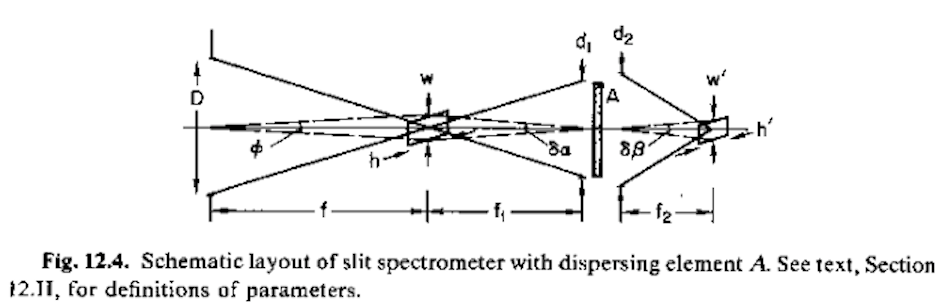
\includegraphics[width=0.8\textwidth]{slit2.png}
\end{figure}
A conventional spectrograph has each of the following:
\begin{itemize}
    \item collimator
    \item dispersive element
        \begin{itemize}
            \item prism
            \item diffraciton grating (most common in astronomy)
        \end{itemize}
    \item camera to refocus the light
    \item detector
\end{itemize}
The performance of a spectrograph is characterized by the \textit{dispersion},
which gives the amount that different wavelengths are separated, and the
\textit{resolution}, which gives the smallest difference in wavelength that two
different monochromatic sources can be separated.

\mydate{Monday, April 25}

\paragraph{Dispersion:}
\mynotes{How much are different wavelengths separated?}
The dispersion depends on the characteristic of the dispersing element. Various
elements can be characterized by the angular dispersion, d$\theta$/d$\lambda$,
or alternatively, the reciprocal angular dispersion, d$\lambda$/d$\theta$. In
practice, we are often interested in the linear dispersion, d$x$/d$\lambda$ =
$f_{2}d\theta$/d$\lambda$ or the reciprocal linear dispersion, d$\lambda$/d$x$
= $\frac{1}{f_{2}}$d$\lambda$/d$\theta$ where the latter is often referred to
simply as the dispersion in astronomical contexts, and is usually specified in
\AA{}/mm or \AA{}/pixel.

If the source being viewed is extended, it is clear that any light which comes
from regions parallel to the dispersion direction will overlap in wavelength
with other light, leading to a very confused image to interpret. For this
reason, spectrographs are usually used with slits or apertures in the focal
plane to restrict the incoming light. Note that one dimension of spatial
information can be retained, leading to so-called \textit{long-slit}
spectroscopy. If there is a single dominant point source in the image plane, or
if they are spaced far enough (usually in combination with a low dispersion)
that spectra will not overlap, spectroscopy can be done in \textit{slitless}
mode. However, note that in slitless mode, there can be a significant impact
from sky emission.

\paragraph{Resolution}
\mynotes{Can two wavelengths be distinguished?}
The resolution depends on the width of the slit or on
the size of the image in slitless mode, because all a spectrograph does is
create an image of the focal plane after dispersing the light. The ``width'' of
a spectral line will be given by the width of the slit or the image, whichever
is smaller. In reality, the spectral line width is a convolution of the
slit/image profile with diffraction. The spatial resolution of the detector may
also be important.

Note that \textit{throughput} may also depend on the slit width, depending on
the seeing, so maximizing resolution may come at the expense of
throughput. Throughput = seeing + slit width.

Given the width, $\omega$, and height, $h$, of a linear slit,
we can get an \emph{image} of the slit with width $\omega'$ and
height $h'$:
\[
    h' = h\frac{f_{2}}{f_{1}}
    \]
Or for an angular width, $\phi = \omega/f$,
(where $f$ is the focal length of the telescope) and height:
$\phi' = h/f$:
$$ \omega' = r\omega\frac{f_{2}}{f_{1}} $$
where we have allowed that the dispersing element might
magnify/demagnify the image in the direction of dispersion by a factor
$r$, which is called the anamorphic magnification.

Using this, we can derive the difference in wavelength between two
monochromatic sources which are separable by the system.
$$ \delta\lambda = \omega'\frac{\textrm{d}\lambda}{\textrm{d}x} $$
$$ \delta\lambda = r\omega\frac{f_{2}}{f_{1}}\frac{\textrm{d}\lambda}{\textrm{d}x} $$
The bigger the slit, the lower the resolving power.
The resolution is often characterized in dimensionless form by{$$
    R \equiv \frac{\lambda}{\delta\lambda} =
    \frac{\lambda{f_{1}}}{r\omega{f_{2}}\left(
        \textrm{d}\lambda/\textrm{d}x\right)}
$$}Note that there is a maximum resolution allowed by diffraction. This
resolution is given aproximately by noting that minimum angles which
can be separated is given by approximately $\lambda/d_{2}$,
where $d_{2}$ is
the width of the beam at the camera lens, from which the minimum
distance which can be separated is:{$$
    \omega_{min} = f_{2}\frac{\lambda}{d_{2}}
$$}The slit width which corresponds to this limit is given by:{$$
    \omega' = r\omega\frac{f_{2}}{f_{1}} = f_{2}\frac{\lambda}{d_{2}}
$$}or{$$
    \omega = \frac{f_{1}}{r}\frac{\lambda}{d_{2}}
$$}and the maximum resolution is{$$
    R_{max} =
    \frac{d_{2}}{f_{2}\left(\textrm{d}\lambda/\textrm{d}x\right)} =
    d_{2}\frac{\textrm{d}\theta}{\textrm{d}\lambda}
$$}
\subsection{Astronomical spectrographs}
\begin{itemize}
    \item Slitless spectographs.
    \item Long slit spectrographs
    \item Image slicers: preserving resolution and flux.
    \item Fiber spectrographs: multiobject data.
    \item Slitlets: multiobject data.
    \item Integral field spectrographs.
\end{itemize}

\subsection{Dispersing elements}
\subsubsection{Prisms}
Perhaps the simplest conceptual dispersing element is a prism, which
disperses light because the index of refraction of many glasses is a
function of wavelength. From Snell's law, one finds that:{$$
    \frac{\textrm{d}\theta}{\textrm{d}\lambda} =
    \frac{t}{d}\frac{\textrm{d}n}{\textrm{d}\lambda} $$
}where $t$ is the base length, and $d$ is the beamwidth. Note that prisms
do not have anamorphic magnification ($r=1$). The limiting resolution
of a prism, from above is:{$$
    R_{max} = \frac{d_{2}}{f_{2}(\textrm{d}\lambda/\textrm{d}x)} =
    d_{2}\frac{\textrm{d}\theta}{\textrm{d}\lambda} $$$$
    R_{max} = t\frac{\textrm{d}n}{\textrm{d}\lambda}
$$}For many glasses, $\textrm{d}n/\textrm{d}\lambda \propto \lambda^{-3}$.
\begin{figure}
    \centering
    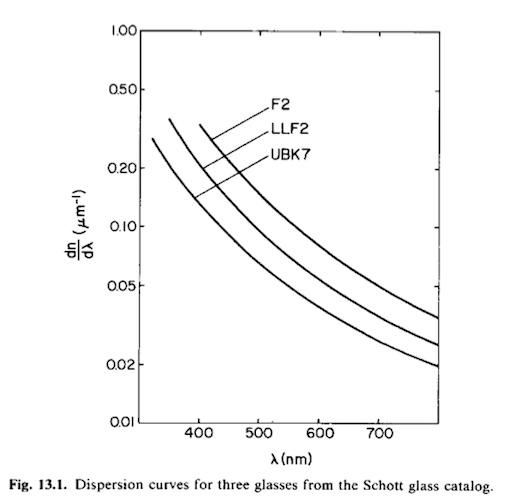
\includegraphics[width=0.8\textwidth]{curves.png}
\end{figure}
So dispersion and resolution are a function of wavelength for a prism.
In addition, the resolution offered by a prism is relatively low
compared with other dispersive elements (e.g.\ gratings) of the same
size. Typically, prisms have $R < 1000$. Consequently, prisms are rarely
used as the primary dispersive element in astronomical spectrographs.
They are occasionally used as cross-dispersing elements.

\subsubsection{Gratings}
Diffraction gratings work using the principle of multi-slit
interference. A diffraction grating is just an optical element with
multiple grooves, or slits (not to be confused with the slit in the
spectrograph). Diffraction gratings may be either transmissive or
reflective. Bright regions are formed where light of a given
wavelength from the different grooves constructively interferes.
\begin{figure}[ht]
    \centering
    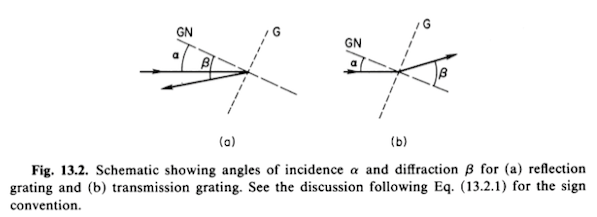
\includegraphics[width=0.6\textwidth]{angle.png}
\end{figure}
The location of bright images is given by the
\emph{grating equation}:{$$
    m\lambda = \sigma\left(\sin\theta + \sin\alpha\right)
$$}for a reflection grating, where
\begin{itemize}
    \item $\sigma$ is the groove spacing
    \item $m$ is the order
    \item $\alpha$ is the angle of incidence
    \item $\theta$ ($\beta$ in picture above) is the angle of diffraction
\end{itemize}
$\alpha$ and $\theta$ are measured relative to the normal to the grating surface.

The dispersion of a grating can then be derived:{$$
    \frac{\textrm{d}\theta}{\textrm{d}\lambda} =
    \frac{m}{\sigma\cos\theta} $$
}The dispersion is larger at higher order, and for a
finer ruled grating. The equation can be rewritten as{$$
    \frac{\textrm{d}\theta}{\textrm{d}\lambda} =
    \frac{\sin\theta + \sin\alpha}{\lambda\cos\theta} $$
}from which it can be seen that high dispersion can also be achieved by
operating at large values of $\alpha$ and $\theta$. This is the
principle of an echelle grating, which has large $\sigma$, and
operates at high $m$, $\alpha$ and $\theta$, and gives high dispersion
and resolution. An advantage of this is that one can get a large
fraction of the light over a broad bandpass in a series of adjacent
orders.

Typical gratings have groove densities between 300 and 1200 lines/mm.
Echelle gratings have groove densities between 30 and 300 lines/mm.

The anamorphic magnification for a grating can be derived by looking
at how $\theta$ changes with $\alpha$ at fixed $\lambda$:{$$
    r = \frac{\textrm{d}\theta}{\textrm{d}\alpha} =
    \frac{\cos\alpha}{\cos\theta} =
    \frac{d_{1}}{d_{2}} $$
}where the $d$'s are the beam diameters. Note that higher resolution
occurs when $r < 1$, or $\theta < \alpha$.

(insert figure here)

The limiting resolution can be derived:{$$
    R_{max} = \frac{d_{2}}{f_{2}\left(\textrm{d}\lambda/\textrm{d}x\right)} =
    d_{2}\frac{\textrm{d}\theta}{\textrm{d}\lambda} $$$$
    R_{max} = \frac{d_{2}m}{\sigma\cos\theta} = \frac{mW}{\sigma} = mN $$
}where $W$ is the width of the grating ($=d_{2}/\cos\theta$), and $N$ is
the total number of lines in the grating.

Note that light from different orders can fall at the same location,
which can be confusing. This occurs when:{$$
    m\lambda' = (m_1)\lambda $$
}or{$$
    \lambda' - \lambda = \frac{\lambda}{m} $$
}The order overlap can be avoided using either an \emph{order-blocking filter}
or by using a cross-disperser. The former is more common for small $m$, the
latter for large $m$.

Comparison between gratings operating in low order, gratings operating in
high order, and prisms shows that higher resolution is
available from gratings, and that echelles offer higher resolution
than typical low-order gratings.

\emph{Grating efficiency} is the fraction of incident light
directed into a given diffracted order. For a
simple grating, less light is diffracted into higher orders. However,
a grating that maximizes the light put into any desired order can be
constructed by \emph{blazing} the grating, which involves tilting each
facet of the grating by some blaze angle. The blaze angle is chosen to
maximize the efficiency at some particular wavelength in some
particular order; it is set so that the angle of diffraction for this
order and wavelength is equal to the angle of reflection from the
grating surface. The \emph{blaze function} gives the efficiency as a function
of wavelength.

A special case of high efficiency is when the angle of incidence
equals the angle of diffraction, i.e.\ the diffracted light at the
desired wavelength comes back to the same direction of in the incoming
light. This is called the Littrow configuration; high efficiency
spectrographs often try to work close to this configuration.

(insert figure here)

Typical peak efficiencies of reflective diffraction gratings are of
order 50-80\%. Recently, a new technology for making diffraction
gratings, volume phase holographic
(\href{http://www.kosi.com/Holographic_Gratings/vph_ht_overview.php}
{VPH}) gratings, as been developed,
and these are attractive because they offer the possibility of very
high efficiencies ($>$ 90\% peak efficiency).

\subsubsection{Grisms}

A grism is a combination of a prism and a diffraction grating. These
are combined such that light is dispersed, but light at a chosen
central wavelength passed through the grism with direction unchanged.
This feature allows grisms to be placed in an imaging system (e.g., in
a filter wheel) to provide a spectroscopic (usually low resolution)
capability.

\rule{\textwidth}{0.4pt}
\subsection{Operational items: using a spectrograph}
{\small\hfill\textcolor{date}{Date?}}

Choice of dispersion: wavelength coverage vs.\ dispersion/resolution,
available gratings, etc. Using grating tilt to select wavelength
range.

Choice of slit width (science, seeing).

How to put object in slit. Imaging the slit. Slit viewing cameras.

(DEFER FOLLOWING TO SECTION ON DATA REDUCTION???)

Spectrograph calibration (not including basic detector calibration, to
be discussed soon).

Wavelength calibration: correspondance between pixel position (in
wavelength dimension) and wavelength. Arc lamps, wavelength solutions.
Subtleties: extrapolation, line curvature, flexure (using skylines to
calibrate).

Flux calibration: relative fluxes at different wavelengths.
Spectrophotometric standards. Subtleties: differential refraction

Spectral extraction: object extraction and sky subtraction.
Subtleties: S-distortion, differential refraction: spectral traces.
Issues: variation of focus along slit and implications for sky line
subtraction, scattered light.

Relative fluxes along slit: slit width variations.

Examples of typical spectra: line lamps, flat fields, stellar spectra,
galaxy spectra. Night sky emission.

\subsection{Non-dispersive spectroscopy}

It is also possible to use interference effects to measure spectral
energy distributions instead of a dispersing element. The Fabry-Perot
is an example of such a type of instrument, although it does not
record all wavelengths simultaneously.

(insert figure here)

Another instrument which uses interference to infer spectroscopy
information is the Fourier Transform Spectrometer (FTS), which is
basically a scanning Michaelson interferometer. The light from the
source is split into two parts using a beamsplitter. One part of light
is reflected off a fixed flat mirror and the other is reflected off a
mirror which can be moved laterally. The two images are combined to
form fringes. The fringe pattern changes as the path length of the
second beam is changed. The intensity modulation for a given
wavelength ($\lambda$) or wavenumber ($k = 2\pi/\lambda$) is
given by:{$$
    T\left(k,\Delta{x}\right) = \frac{T_{max}}{2}
    \left[a + \cos\left(2k\Delta{x}\right)\right]
$$}and the flux after integrating over all wavelengths is:{$$
    F\left(\Delta{x}\right) =
    C\int{I(k)T(k,\Delta{x})\textrm{d}k} =
    C\int{I(k)\cos(2k\Delta{x})\textrm{d}k}
$$}where $I(k)$ is the input spectrum. Consequently it is possible to
recover the input spectrum by taking the Fourier cosine transform of
the recorded intensity. In practice, a discrete Fourier transform is
used.

The FTS requires scanning in path spacing. But unlike the Fabry-Perot,
it yields information on intensity at all wavelengths simultaneously.

\newpage
\mydate{Monday, May 2, 2016}
\section{Detectors}
\subsection{Basic Principles and Properties}
Detectors work because they are made of material that interacts
with photons. Three general types, based on what is generated
by the photon:
\begin{description}[labelwidth=10em, leftmargin=12em]
    \item [Photographic detector] chemical reaction
    \item [Photomultiplier/photon counter] event, usually detected
        in real time. Electrons are rapidly accelerated toward anode
        by photon, then more electrons are excited and accelerate, and
        so on. High voltage. These are \emph{not} imagers.
    \item [Photon collecter] photoelectron, usually (electronically)
        stored for subsequent readout. CCDs are a subset of this type.
\end{description}

In a photon counting device, some fraction of incident photons hit a
photosensitive material and eject a photoelectron. This electron is
amplified numerous times to create a large ``swarm'' of electrons
which is detected as a pulse. Thus, photons are ``counted'' as they
come in. Simple photomultipliers do not retain any information about
the location on the detector where the photon hits. There are some
modern devices, however, called microchannel plates, which are
essentially arrays of small photomultipliers where positional
information can be obtained; one of the more common of these is called
a MAMA (Multi-Anode\ldots something),
and exists in several instruments on the Hubble Space
Telescope. Traditional photomultipliers were the workhorse of
photometry from the 50's to the late 70's. More recently, a more
sensitive type of photon counter, called an avalanche photo-diode, has
been used.

Photon collecting array detectors are in more common usage today. In
these devices, incoming photons create photoelectrons which are
trapped in local potential wells. The amount of energy needed to eject
a photoelectron depends on the type of material used. In the optical,
silicon provides a good choice, but the excitation energy for silicon
is too high to be used in the infrared. In the IR, various different
substances are used, including HgCdTe, InSb, and PtSi. After a
specified amount of time, the photoelectrons are ``counted''. The
method by which this is done differs between different types of
arrays. In CCDs, the charge is physically clocked down columns of the
device, a single row at a time (a parallel transfer) then read out of
serial register; CCDs are inherently asymmetric in rows and columns.
In IR devices, each pixel is read individually, in sequence.
\textcolor{myBlue}{Material: semiconductor. In optical, pure silicon
is used, which isn't sensitive at wavelengths greater than $\sim$
1 $\mu$m. At 1$\mu$m, ``barely'' enough energy. Other materials used
in IR\ldots First two are sensitive out to about 2.5 $\mu$m, last one
to $\sim$ 5 $\mu$m (see book in library about the physics here!)}

Detectors are characterized by a variety of different important
quantities that should be considered when buying them\ldots
what do you need for your science? The ``Biggies'':
\begin{description}
    \item [Quantum efficiency] fraction of photons detected, usually
        a function of wavelength. Typical values:
        \begin{itemize}
            \item photographic: $\sim$ 0.1 \%
            \item photomultiplier: $\sim$ 10-20 \%
            \item array detector: $\sim$ 20-90 \%
        \end{itemize}
    \item [Size and resolution elements] (given that optics can be used
        to change the scale, the number of resolution elements may be
        more critical):
        \begin{itemize}
            \item photographic: large (many inches), good resolution
            \item photomultiplier: several inches, no resolution
                (though there are arrays of photomultipliers, e.g.
                MAMA). APDs (?) have very small collecting areas.
            \item Array detector: individual detectors started out
                small but are continually growing. The largest current
                CCDs are around 2.5 in$^{2}$, wheras the largest IR
                arrays are roughly 1 in$^{2}$. Larger effective sizes
                are now available (for CCDs) because modern devices
                are made to be ``buttable'', i.e.\ several can be
                placed side by side with only very small gaps between
                them. Pixel sizes of array detectors are typically
                15-25 microns (although arrays with smaller pixels are
                very common, e.g., for digital camera, etc,
                applications, they are less frequently used in
                astronomy because they generally don't provide a good
                match to telescope scales).
        \end{itemize}
    \item [Discovery efficiency] product of sensitivity and area.
    \item [Readout effects] The process of counting electrons is never totally
        exact, so noise is introduced. Generally this is at a level of 1-100
        electrons rms. Readout effects can come in two different forms:
        \begin{enumerate}
            \item pattern noise: introduced in the readout process, but has
                some spatial correlation. \textit{Fixed} pattern noise has the
                same spatial pattern over the detector from exposure to
                exposure, and thus can be corrected. \textcolor{myBlue}{If the
                pattern noise is not fixed, it changes every time exposure is
                read out.}
            \item random noise: what people usually refer to as readout noise.
                If, instead of photoelectrons, photon \emph{events} are counted
                (photomultiplier), there is no readout noise;
                \textcolor{red}{this is the key advantage of photon counters.}
        \end{enumerate}

        \textcolor{date}{Wednesday, May 4, 2016} Should add some margins to
        these notes\ldots

    \item [Dark current] Electrons in a given substance will be moving
        around at speeds correlated with the operating
        temperature of the device. If there is enough thermal motion,
        an electron can be liberated from the substance and
        then counted as a (spurious) photon detection. This is called
        dark current. Devices with lower photoelectric threshholds
        (used at longer wavelengths) are more susceptible to dark
        current, thus they must be operated at a colder temperature.
        CCDs are typically operated between -70$^{\circ}$C and
        -120$^{\circ}$C, IR arrays
        are colder (77K for liquid N$_{2}$, 4K for liquid He). Dark current
        can be subtracted using calibration data, but note that
        there is still the Poisson \emph{noise} associated with the dark
        current, so even with dark subtraction, additional noise is
        generated.
    \item [Linearity] relation between number of output electrons and
        input photons. In a fully linear detector,
        the slope of the relation is given by the quantum
        effeciency, which can be considered as a function of the count
        level for \emph{non}linearity.
        \begin{itemize}
            \item photographic: nonlinear
                (\href{https://en.wikipedia.org/wiki/Sensitometry}
                {characteristic curve})
            \item photoelectric: linear except for dead-time correction.
                A dead-time correction applies for bright sources; if
                two photons arrive essentially simultaneously, they
                will only be counted as a single photon.
            \item array detector: CCDs \emph{usually} linear up to
                50-90\% of full well. IR arrays are usually slightly
                nonlinear over their entire range, but repeatably so.
        \end{itemize}
    \item [Full well] maximum number of photons possible to detect.
        \begin{itemize}
            \item photographic: limited by number of gains
            \item photomultiplier: unlimited
            \item array detector: $\sim$ 100,000 photons
        \end{itemize}
\end{description}
Other possible effects/issues:
\begin{itemize}
    \item Defects. Most detectors are not perfect; there are often small
        regions which are unusable because of very low quantum efficiency,
        blocked columns, etc. Many devices are rejected for astronomical use
        because of too many defects. \mynotes{dead pixels - no response at all.
        sensitivity changes from pixel to pixel (reason for flats).}
    \item Modulation transfer function. In some detectors at some wavelengths,
        charge deposited at one location can be spread over a wider region,
        leading to degradation of image quality.  This is often most notable at
        long wavelengths in CCDs, where one can see moderately large halos
        around point sources. This is usually due to the penetration of long
        wavelength photons to the substrate of the device from which they can
        be reflected back.
        \mynotes{characterizing the \emph{size} of an image.}

        A related effect is fringing on chips, which results from interference
        of monochromatic (not broadband) incident light that is reflected from
        the substrate, which is relevant because the night sky spectrum
        contains strong monochromatic features. Since the substrate surface is
        not perfectly flat, this can lead to irregular patterns in the
        background. Examples: DIS red fringing, 1m i band imaging. The details
        of fringing depend on specifics of the chip construction, and fringing
        effects can be mitigated in some cases. \mynotes{what back of device
        looks like, hard to deal with this, don't see it when the moon is up,
        amount of fringing is proportional\ldots also depends on what direction
        you're facing.}

    \item Readout speed: typically 25 microsec/pixel for array detectors.
        However, the chips can in many cases be read at a variety of speeds. In
        general, when chips are read faster, the readout noise increases.
        Larger chips now often have multiple readout channels, so several
        regions of the chip can be read simultaneously, decreasing the total
        readout time.
        \mynotes{ccd: charge transferred down, then across to \emph{amplifier},
        split into four parts (quad-channel readout vs.\ single channel
        readout.) More expensive though\ldots}
    \item Saturation behavior. When full well is reached, the chip is
        said to be saturated. In some array detectors, especially
        CCDs, when a given pixel is saturated, additional charge often
        leaks into adjacent pixels, usually into adjacent rows rather
        than columns because of the construction of the CCD\@.
        Separately from detector saturation, one occasionally sees
        saturation of the readout electrons which can have the effect
        of a saturated pixel affecting the counts in subsequent
        pixels.
    \item Hysteresis generally refers to processes in which the prior
        exposure history of a detector affects subsequent exposures. A
        common example is \emph{residual image}, in which an area of a
        detector which was subject to a very bright source in a
        previous exposure will continue to ``glow'' in subsequent
        exposures. Another form of hysteresis is so-called quantum
        efficiency hysteresis (QEH) in which the quantum efficiency of
        the chip changes as a function of previous exposure history.
        One manifestation of this effect has been used by astronomers,
        mostly with older CCDs; for some reason, when these CCDs were
        subjected to an extended influx of ultraviolet light, their
        optical quantum efficiency was found to be increased, and to
        stay increased at a stable level as long as the chip was kept
        cold. This led to the practive of ``UV-flooding'' CCDs as they
        were being cooled.
    \item Reciprocity: sensitivity changes as a function of photon
        incidence \emph{rate}. Exists in photographic plates,
        \emph{maybe} in some
        array detectors? Dead-time correction is a reciprocity
        failure.
\end{itemize}
\subsubsection{Digitization}
In array detectors, after the charge is collected and read out, it is
sent through a chain of electrons which
\textit{digitizes}\footnote{Online definition: convert into a digital
form that can be processed by a computer}
the signal, often
after amplifying it. The digitization is made by a device known as an
A/D convertor; these work by comparing an input signal with a set of
reference voltages which successively differ by factors of two. Thus
an input signal is translated into a series of bits depending on
whether the input voltage exceeds a series of reference voltages.
Typical A/D correctors in use in astronomy consider 16-bits.

The digital signal which comes out of the CCDs is variously referred to as
one of the following:
\begin{itemize}
    \item counts
    \item digital numbers (DN)
    \item analog-to-digital units (ADU).
\end{itemize}
\paragraph{Gain:}
The number of output counts is related to the number of input counts by a
constant which depends on the amplification in the electronics. The
amplification factor is known by most people as the gain, but
astronomers define the gain of a device by the \textit{number of input
electrons divided by the number of output counts} (i.e., the inverse
gain); this ``astronomers'' gain is specified in units of e-/DN.
Because the number which we receive from the electronics chain differs
from the number of input electrons (i.e, the number of detected
photons), the calculation of noise must take this into account. The
photon counting noise (rms) is given by the square root of the number
of detected photons. The number of detected photons is given by GC,
where G is the (inverse) gain and C is the number of detected counts.
Consequently, the noise in electrons is $ \sqrt{{GC}}$, and in units
of counts is given by  $ \sqrt{{C/G}}$. This is apart from readout
noise; the latter is usually specified in units of electrons, giving a
total noise in electrons of  $ \sqrt{{GC+\sigma_{rn}^{2}}}$, or, in
units of counts, by  $ \sqrt{{C/G+\sigma_{rn}^{2}/G^{2}}}$.

A/D converters can only measure a positive incoming signal. At low
light levels, the true input signal can be negative in the presence of
readout noise. To avoid trucation of the negative signals, a constant
voltage, called the bias, is added to the signal before it passes
through the A/D. This bias must later be removed to preserve the
correct count ratios between different sources; this is generally
accomplished in CCDs by using the overscan region of the image.

A/D convertors can introduce small systematic errors in recorded count
rates if the reference voltages are not carefully controlled.


\subsubsection{Dynamic range}
A detector system can be characterized by its dynamic range, which is
the ratio of the signals of the brightest and faintest sources which
can be detected (with some definition of ``detection''). At the bright
end, the system is limited by either the full well of the detector (or
the number of electrons at which the detector goes significantly
non-linear), or alternatively by the limitation of the A/D convertor
(e.g., if an A/D convertor has 16 bits, you can never see counts
higher than 2$^{16}$ - 1 = 65535). At the faint end, the system is limited
either by the A/D convertor (you can't detect less than one count), or
by the readout noise (source buried by readout noise cannot be
detected). The gain of a system is often set to maximize the dynamic
range; if the readout noise is $ \sim$ 10 electrons, one can maximize
dynamic range by digitizing the signal by several electrons/DN if the
detector has sufficient full well.


\subsubsection{Determining gain and readout noise}
\subsection{CCDs}
\subsection{IR detectors}
\subsection{UV and other detectors}

\section{Data reduction: details and subtleties}

\section{Photometry}

(All lecture notes from this section copied from website. Not edited
at all yet).

Consider techniques for stellar photometry, surface photometry,
calibration of broad band and emission line photometry.


\subsection{Aperture photometry}
In aperture photometry, we simply identify stars and add up all of the
light in the surrounding pixels. The light is spread over several
pixels in a form given by the point spread function PSF(i, j). We must
also measure the background and subtract its contribution to the sum.

Error estimation: we're going to sum over pixels. First just consider
the object aperture:
\[
    \]
where the sum is over N pixels, and B is the background per pixel. To
get the true signal S, N would need to approach infinity since the
stellar profile continues out to great distances. In practice,
however, we choose N such that a repeatable fraction of light falls
within the N pixels independent of exposure. Next, we want to
determine the error in our measurement of S. The noise is

\[
    \]
which is just
\[
    \]
Now we have to consider how we will estimate B. In the simplest case,
we just go away from the star and take then mean level. Generally, we
want to minimize effects of any nonuniform background, so we consider
an annulus around the star. If this annulus contains Na pixels, then


\[
    \]
and
\[
    \]
From this we see that errors in determining the background are small
contributors to the total error in the star if Na > > N, and generally
that is the case. If the errors in determining the background are
negligible, then

\[
    \]
which is an important result that we have seen before, but here the
area is explictly given in terms of a number of pixels.
Using this, one can consider the optimal choice of aperture. As the
aperture size increases, you get a increase in total signal, but also
an increase in background, so the change in S/N depends on how bright
the star is relative to background. The optimal choice of aperture
will depend on the brightness of the star: a larger aperture will be
better for brighter stars, a smaller aperture for fainter stars. But
also recall that we don't want to use a too small aperture or else we
won't be able to compare results from different frames because of
changes in the PSF.

This leads to the commonly used technique of using small apertures for
all of the stars on the frame, but large apertures for a few bright
stars. The few bright stars are assumed to have representative PSFs
for this frame, so all of the small aperture measurements can be
aperture corrected to large aperture measurements without the increase
in noise you would get if you actually used a large aperture. Note
that you can't go arbitrarily small as you will eventually run into
the problem of PSF variations across the frame if for no other reason
than any small dependences on pixel centering.

In fact, you can do better for S/N if you use additional information.
If you know the shape of the PSF, you can use this information to fit
your stellar image, increasing the S/N in the process. Simple linear
least squares argument, if you know PSF and position accurately, leads
to
\[
    \]
where
\[
    \]
Note that you'll improve S/N, but only if your assumption that your
knowledge of the PSF is good is valid. This naturally leads into the
next area of stellar photometry in crowding fields, when you are
forced into fitting the PSF whether you like it or not.


It is customary to express the observed number of counts in a frame in
terms of an instrumental magnitude:

\[
    \]
\subsection{Crowding}
Clearly, the above technique breaks down as you have more than a few
stars in your frame for two reasons: the stars may have overlapping
light, and there may be stars in your sky annuli. This leads to
techniques for crowded field photometry, a complicated subject which
we'll just review quickly.

In crowded field photometry, the idea to that you have to solve for
the brightnesses of overlapping stars while considering the
contribution of neighboring stars. To do this requires that you have
information about the point spread function. There are several
possibilities for how you might consider accounting for neighbors:
\begin{itemize}
    \item Fit all stars that have an effect on each other simultaneously.
        Unfortunately, in very crowded fields, this can lead to huge groups of
        stars to be considered simultaneously, which can be computationally
        difficult, if not impossible. (DAOPHOT NSTAR)
    \item Fit each star independently, but iterate the fit: at each iteration,
        subtract the contribution for all neighbors before fitting each star.
        (DOPHOT)
    \item Use some combination of the above. (DAOPHOT ALLSTAR)
\end{itemize}
Simply, the technique consists of: finding stars, finding the PSF,
grouping the stars, and simultaneously fitting for stellar
brightnesses and positions. You almost certainly have to do positions
because your initial estimates will probably be biased by neighbors.
You also might consider fitting for the background as well. We'll
consider each one of the steps in order:

\subsubsection{Finding stars}
Need to consider automation because of completeness issues, not to
mention tedium.

Look for peaks; clearly need to consider background noise, so look for
peaks above some noise threshold. More sublety: look for peaks which
look like they have the right shape to be stars. Matched detector
algorithm. Shape parameters, e.g. sharpness, roundness for additional
spurious object rejection.

\subsubsection{Finding the PSF}
Find bright isolated stars. Tabulate the PSF. However, rememeber that
you're going to have to use this PSF to estimate brightnesses for
other stars, so you'll need to be able to interpolate it accurately.
Consider using a functional fit to PSF, possibly carry along residuals
as well.



\subsubsection{Grouping stars}
As discussed above, either consider all stars that overlap, or iterate
each star individually with improved neighbor subtraction at each
iteration.



\subsubsection{Fitting stars}
For all pixels under consideration, compare observed values with first
guess values. Use residuals to refine your guesses (nonlinear least
squares). Continue iterating until parameters converge.



\subsubsection{Subleties}
Sky estimation. Mode approx: 3*median - 2 * mean.

Multiple iterations of entire procedure to improve PSF by subtracting
neighbors, also to find new stars under wings of other stars.

Multiple colors/frames simultaneously.

Completeness. Function of crowding. Spurious detections as well as
misses.

Averaging measurements. Averaging mags not the same as averaging
counts. Beware of weighted means if you use estimated errors, because
these can be biased.


\subsection{Atmospheric extinction}

f you want to compare brightnesses of stars in different observations,
you need to correct for the different absorption of the earth's
atmosphere as a function of airmass. Note that if you are just
comparing brightnesses within individual frames (differential
photometry), correcting for atmospheric absorption isn't necessary, to
the extent that the absorption is the same for all objects in the
frame.

We've already desribed the absorption/scattering effects of earth's
atmosphere:

F = F0exp(- $\displaystyle \tau_{0}^{}$X)
or
m = m0 +1.086$\displaystyle \tau_{0}^{}$X
m = m0 + kX
m0 = m - kX
where k is the extinction coefficient. As we've discussed, this can
vary from night to night, so if you're interested in accurate
photometry (better than a couple percent), you need to measure it on
your night. Also remember that the extinction coefficient is
wavelength dependent, so you need a separate number for each filter.
It's also critical to measure this to check for photometric weather:
even if you don't require a few percent, if there are clouds you might
get a lot worse! So you need to check.
The extinction coefficient can be determined by making multiple
observations of a star at different airmasses. Then you can solve for
k and m0 using least squares. Note that you need to sample a good
range of airmasses to get good leverage on the fit, and you should
bracket the airmasses of all of your program objects.

When doing broad-band work, however, there's an additional subtlety
because of the wavelength dependence. Two different stars might have
different extinction coefficients in the same filter because the stars
might have very different colors, which has an effect if the filter
bandpass is broad. This problem can be solved by using second order
extinction coefficients, where the extinction is a function not only
of the airmass, but also of the stellar color:
\[
    m = m_{0} + kX + k_{2}(color)X
    \]
where color can be either an observed or a known color for the star.
Second order effects will have more importance in the limits of
broader bandpasses, working with objects of extreme colors, and/or
working with bandpasses in which the extinction coefficient varies
rapidly within the bandpass (e.g., the near-UV).
Another important thing to remember is that although we correct for
the effects of the Earth's atmosphere using extinction coefficients,
the actual response function of an imaging system includes the
wavelength-dependent response of the Earth's atmosphere, which varies
depending on airmass. If one wants to determine an ``average''
wavelength response of a system, one probably wants to include the
effects of the atmosphere at some ``typical'' airmass, and then
correct the photometry to this airmass; for example, this is what is
done by the SDSS photometric pipeline, where all photometry is
corrected to an airmass of 1.3.

Using the above formalism, you have to solve for extinction
coefficients plus a magnitude for every star you observe. This
requires a fair bit of observing to constrain all of the parameters.
Clearly, if you can observe stars of known brightnesses, you will have
better constraints on the extinction coefficients. These leads us into
the discussion of standard stars.

\subsection{Standard stars}
Standard stars are required so that different observers are able to
compare results with each other. The reason this is true is because
every observational setup is likely to have different response
functions, so the same stars will not be observed to have the same
brightnesses (even relative brightnesses!) with each separate setup.
Differences in response come from many factors: size and condition of
the telescope optics, number and type of optics in the system,
bandpass and quality of the filter, response function of the CCD, etc.
In addition, it is very difficult to measure all of these responses in
any absolute sense, so it is almost impossible to go straight from
observations to inferences about physical fluxes in absolute units.

To get around these problems, systems of standard stars have been set
up so observers can calibrate any new observations against the known
brightnesses of the standard stars. A standard system is just a
more-or-less arbitrary choice of one particular instrumental setup,
but is generally one which is very stable and which someone has spent
a lot of observing time establishing. Generally, the standard system
is tied to absolute flux observations of some primary standard star so
that observations on the standard systems can be converted to physical
fluxes.

Let's consider some examples. First consider two identical systems.
Clearly these will give the same observed flux as each other. Now let
the systems differ only by a multiplicative factor in throughput. Now
the observed fluxes will differ by a constant factor, or a constant
additive factor in magnitudes. With observations of standard stars, it
is straightforward to find the magnitude difference between the
observed magnitude and the standard magnitude to calibrate out this
constant factor. The additive constant in magnitudes is called the
zeropoint.

A slight divergence is called for here to mention that different
packages apply some ``software'' zeropoints to the calculation of
instrumental magnitude just to make the numbers (instrumental
magnitudes) look ``reasonable'' (i.e., familiar). This is no problem
since we determine a zeropoint on top of this to calibrate, but
caution is required if talking about instrumental magnitudes measured
with different software systems!

OK, back to differing instrumental systems. Now let's consider the
more realistic case where the shape of the response curve as well as
the absolute throughput differs from the standard system. Let's
consider a system which has slightly different filters with a
different wavelength cutoff. Now you observe a different number of
counts from the standard system, and the difference depends on the
spectrum of the object you are looking at. Now spectra can differ for
lots of reasons, but the biggest effect is just from spectral slope
differences. If your filter has a shorter wavelength cutoff (on the
red side), then you'll observe less counts than the standard system,
and preferentially less counts for a redder star. To first order, this
can be calibrated out by solving for an additive constant which
depends on the spectrum of the object being looked at. Since we don't
in general know the spectrum, we have to parameterize it by something
we can observe, and the best choice here is the stellar color, as
inferred from observations taken through more than one filter.

Transformation coefficients.
\begin{align*}
    m &= -2.5\log(counts/s) + z_{soft}\\
    m_{0} &= m - kX\\
    M &= m_{0} + t(color) + z
\end{align*}
where capital letters are the magnitude on the standard system, z is
the zeropoint, and t is the transformation coefficent.
The color is generally parameterized by the ratio of the flux at two
different wavelengths, or, in magnitudes, the difference between the
magnitudes. The two wavelengths should be measured near in wavelength
to the wavelength of the filter being corrected; generally, one uses
the bandpass being corrected as one of the wavelenghts and an adjacent
bandpass as the other. For example, when correcting V magnitudes,
people usually use B - V, V - R, or V - I for the color term.

There are two ways to define the color, either in terms of the
observational system or in terms of the standard system. The latter is
slightly preferred for using least-sqaures (small errors on the
independent variable), and also because it allows observations from
different nights to be combined. Note that this formulation does not
require you to know the colors of your objects a priori, it's just
algebra to figure them out as long as you have observations in both
filters.

The use of these first-order transformation coefficients is accurate
as long as your filter system does not differ much from the standard
system, and additionally, that the spectrum of your program objects
does not differ significantly from the spectrum of the standard
objects. The more these conditions are not met, the less accurate the
results. Some additional accuracy in the case of differing systems can
be achieved by using higher order transformation coefficients.
However, even in this case, it is always important to remember that if
the spectrum of the program object differs significantly from the
standards, derived fluxes can be significantly in error.

Certainly, you get to a point when the response of one system is so
different than the response of another system that no transformation
can be determined. In this case, you have two different photometric
systems. In fact, there are several different photometric systems at
use in astronomy today, and each has advantages and disadvantages.

It is common practice to combine the equations for extinction and
transformation coefficients into a single set of equations:
\[
    M_{i} = m_{i} + k_{i}X + t_{i}(M_{i} - M_{j}) + z
    \]
where the subscripts refer to measurements in different filters, and
where I have ignored second order coefficients. The advantage of
combining the equations is that you can use the information about the
known magnitudes of the standard stars for the extinction term, so you
can combine observations of different standards at different airmasses
to derive the extinction coefficient and do not need to observe the
same star at multiple airmasses.
In practice, one observes a set of standards of different colors at
different airmasses. Then one uses least squares techniques to solve
for the values of k, t, and z which minimize the difference between
the observed, transformed, magnitudes and the standard magnitudes.
Then one applies these coefficients to measurements of your program
objects to derive their magnitudes. Clearly, to do so, you must
measure the colors of your program objects by making observations in
more than one bandpass since, unlike the standard stars, the colors of
your program objects are not known a priori.

Note that for calibration of broad-band observations, we do not
require knowledge of the transmission function. Of course, if you have
such knowledge, you could derive synthetic transformations, if you
also know the transmission functions of the standard system. Beware,
however, that getting accurate transmission functions can be very
difficult.

\subsection{Photometric systems}
What are some of the considerations for choosing a photometric system?
One general approach is to consider a broadband system to give a low
resolution approximation to the spectra of objects, regardless of the
details of what objects you might be looking at.

For broadband systems, the most common has been the UBVRI system,
originally established by Johnson in the 1960s. However, even the
UBVRI system has undergone some revisions, and Johnson's original
system is not quite the one used predominantly today.

UBVRI. Cousins RI. Subtleties of Johnson vs. Cousins vs. Landolt.

Gunn system, uvgriz. Additional consideration: night sky brightness.

HST system. Additional consideration: maximum throughput.

Sloan system. Additional consideration: ``clean'' bandpasses.

Choice of photometric system for studies of stars: determination of
temperatures, reddenings, surface gravities, metallicites.

Medium band: Stromgren system, uvby$ \beta$. Others: DDO, Washington.

What goes into a choice of filters to use often involves a tradeoff of
better spectral information vs. S/N considerations. Note that S/N
considerations must include both the errors in the bandpasses being
considered, and also the degree to which different objects are
separated in color space. (possible problem to determine best filter
choice given some sensitivities, astrophysical colors of stars).

Narrow band filters most often used to study emission line objects.



\end{document}
